\documentclass[10pt,a4paper,final]{report}
\usepackage[utf8]{inputenc}
\usepackage{amsmath}
\usepackage{amsfonts}
\usepackage{amssymb}
\usepackage{graphicx}
\usepackage{hyperref}
\usepackage{siunitx}
\usepackage{animate}
\usepackage{listings}
\usepackage[usenames,dvipsnames]{xcolor}
\usepackage{inconsolata}%\usepackage{zi4} \usepackage{upquote}
\usepackage{titlesec} % Used to create a new page with each section.
\usepackage{gnuplot-lua-tikz} % Used for TikZ plots.

\newcommand{\sectionbreak}{\clearpage}
\renewcommand{\thesection}{\arabic{section}}

\hypersetup{
    colorlinks,
    citecolor=red,
    filecolor=blue,
    linkcolor=[rgb]{0,0,0.5},
    urlcolor=yellow
}

\definecolor{CodeRed}{HTML}{EB1717}
\definecolor{CodeGreen}{HTML}{006400}

\begin{document}
\lstset
{
language=Gnuplot,
basicstyle=\ttfamily\scriptsize,
keywordstyle=\bfseries,
showstringspaces=false,
tabsize=4,
numbers=none,
breaklines=true,
breakatwhitespace=true,
showstringspaces=false,
columns=fullflexible, % avoids superfluous spaces
backgroundcolor=\color{gray!10},
keywordstyle=\color{CodeRed},
commentstyle=\color{CodeGreen},
morekeywords={unset, y2range, x2range, fillystyle, do, for, term, multiplot, w, x2tics, y2tics, mx2tics, my2tics}
}

%%%%%%%%%%%%%%%%%%%%%%%%%%%%%%%%%%%%%%%%%
% University Assignment Title Page 
% LaTeX Template
% Version 1.0 (27/12/12)
%
% This template has been downloaded from:
% http://www.LaTeXTemplates.com
%
% Original author:
% WikiBooks (http://en.wikibooks.org/wiki/LaTeX/Title_Creation)
%
% License:
% CC BY-NC-SA 3.0 (http://creativecommons.org/licenses/by-nc-sa/3.0/)
% 
% Instructions for using this template:
% This title page is capable of being compiled as is. This is not useful for 
% including it in another document. To do this, you have two options: 
%
% 1) Copy/paste everything between \begin{document} and \end{document} 
% starting at \begin{titlepage} and paste this into another LaTeX file where you 
% want your title page.
% OR
% 2) Remove everything outside the \begin{titlepage} and \end{titlepage} and 
% move this file to the same directory as the LaTeX file you wish to add it to. 
% Then add \input{./title_page_1.tex} to your LaTeX file where you want your
% title page.
%
%%%%%%%%%%%%%%%%%%%%%%%%%%%%%%%%%%%%%%%%%

%----------------------------------------------------------------------------------------
%	PACKAGES AND OTHER DOCUMENT CONFIGURATIONS
%----------------------------------------------------------------------------------------

\begin{titlepage}

\newcommand{\HRule}{\rule{\linewidth}{0.65mm}} % Defines a new command for the horizontal lines, change thickness here

\center % Center everything on the page
 
%----------------------------------------------------------------------------------------
%	HEADING SECTIONS
%----------------------------------------------------------------------------------------

\vspace*{2cm}
\textsc{\LARGE}\\[2cm] % Name of your university/college
\textsc{\Large }\\[0.5cm] % Major heading such as course name
\vspace*{0.25cm}
\textsc{\large A Collection Of Gnuplot Graphs And Code}\\[0.5cm] % Minor heading such as course title
\vspace*{1cm}
%----------------------------------------------------------------------------------------
%	TITLE SECTION
%----------------------------------------------------------------------------------------

\HRule \\[0.4cm]
\vspace{0.75cm}
{ \huge Gnuplot Examples}\\[0.4cm] % Title of your document
\vspace{0.50cm}
\HRule \\[1.5cm]
 
%----------------------------------------------------------------------------------------
%	AUTHOR SECTION
%----------------------------------------------------------------------------------------

%\begin{minipage}{0.4\textwidth}
%\begin{flushleft} \large
%\emph{Author:}\\
%John \textsc{Smith} % Your name
%\end{flushleft}
%\end{minipage}
%~
%\begin{minipage}{0.4\textwidth}
%\begin{flushright} \large
%\emph{Supervisor:} \\
%Dr. James \textsc{Smith} % Supervisor's Name
%\end{flushright}
%\end{minipage}\\[4cm]

% If you don't want a supervisor, uncomment the two lines below and remove the section above
%\Large \emph{Author:}\\
\vspace*{1cm}
\Large Jean-Luc \textsc{Tambasco} \\ Lisa \textsc{Drummond} \\[3cm] % Your name

%----------------------------------------------------------------------------------------
%	DATE SECTION
%----------------------------------------------------------------------------------------

{\large \today}\\[3cm] % Date, change the \today to a set date if you want to be precise

%----------------------------------------------------------------------------------------
%	LOGO SECTION
%----------------------------------------------------------------------------------------

%\includegraphics{Logo}\\[1cm] % Include a department/university logo - this will require the graphicx package
 
%----------------------------------------------------------------------------------------

\vfill % Fill the rest of the page with whitespace

\end{titlepage}


\tableofcontents

\section{ABC}
Test change.

\section{Animation And Stacked Plot}
\begin{figure*}[htbp]
    \centering
    \animategraphics[autoplay,controls,loop,width=\textwidth]{20}{../Code/animation/animation/animate}{0}{199}
    \caption{The is a stacked plot and animation.  At the time it was made, as far as I know, it only worked in Adobe Reader.}
\end{figure*}
\lstinputlisting{../Code/animation/animation.plt}

\section{Six Plots On A Page And Curve Fitting}
\begin{figure}[!hbtp]
\centering
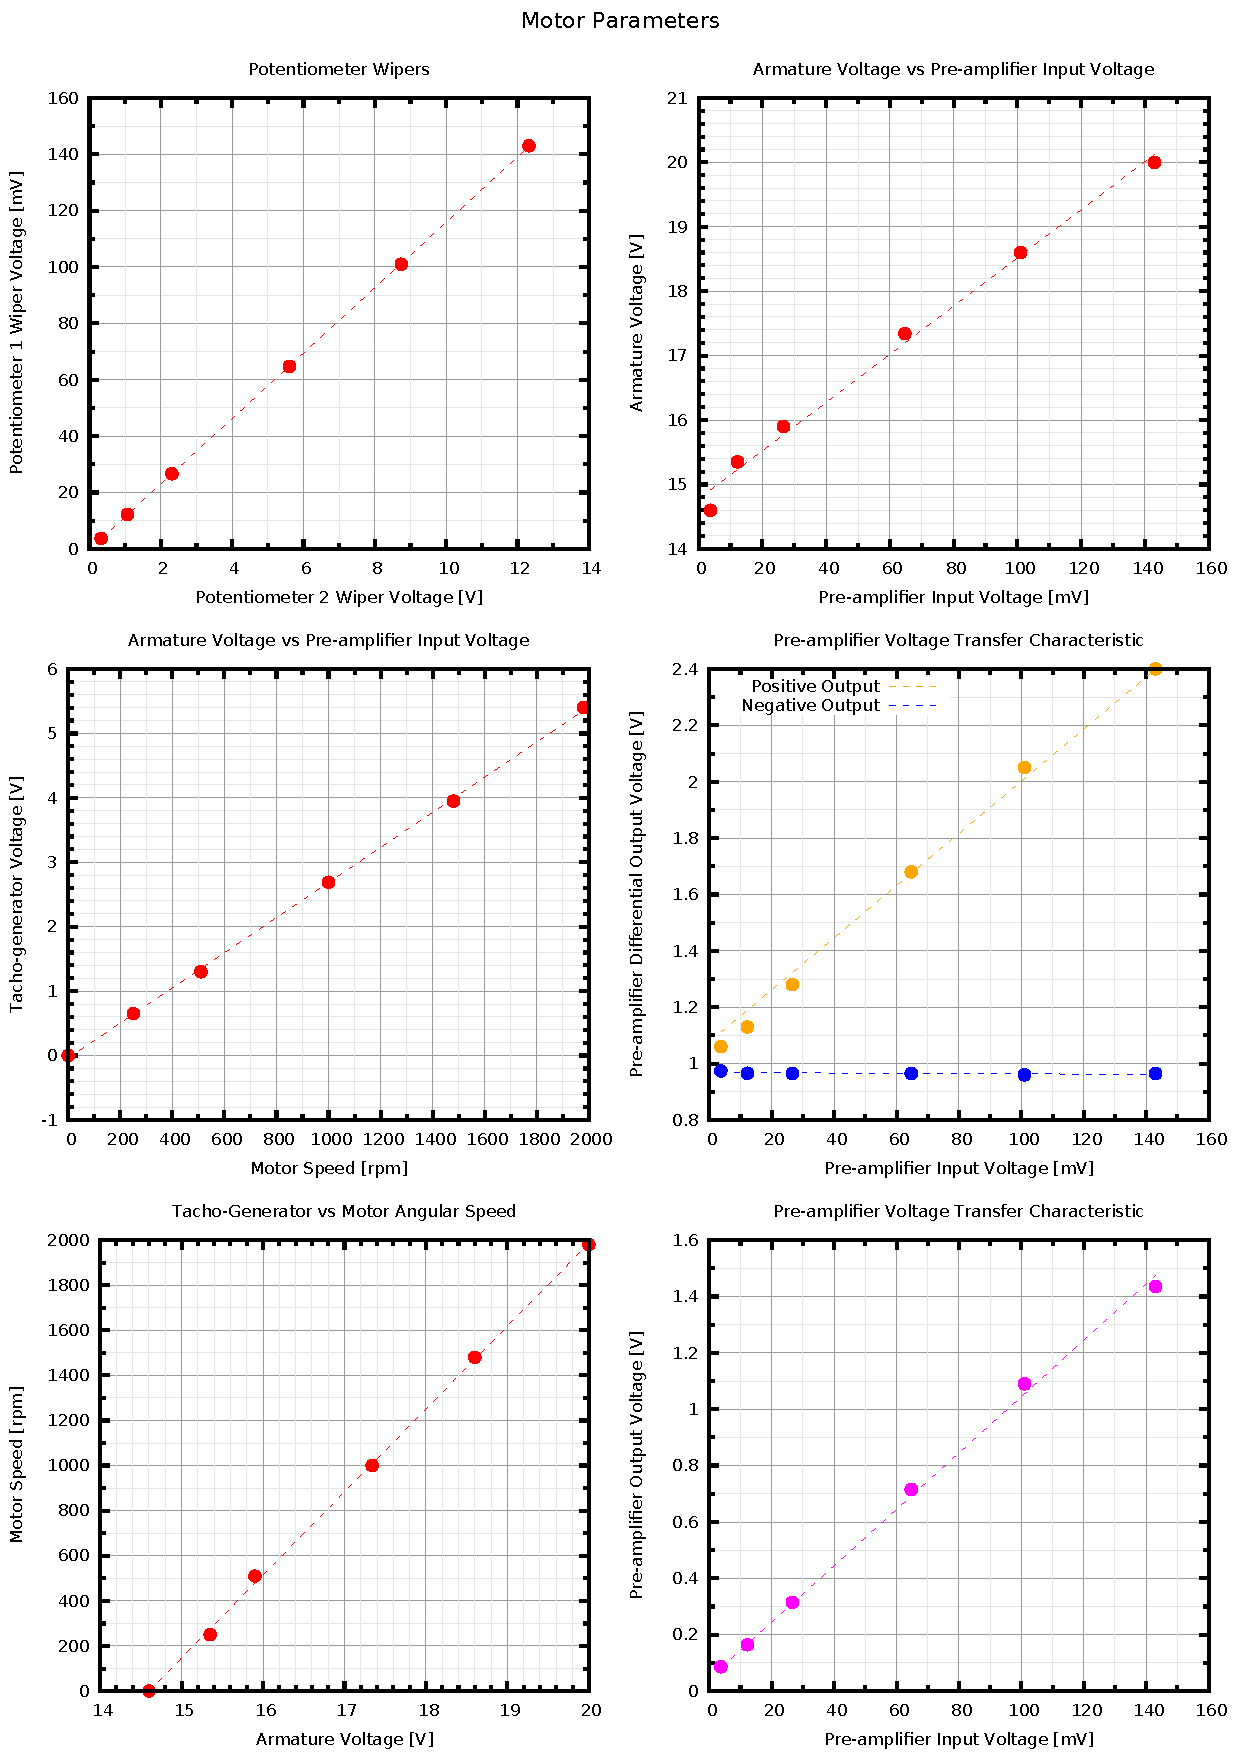
\includegraphics[width=\textwidth]{../Code/MotorGraphGnuplot/OpenLoopMotorPlots.pdf}
\caption{Multiple plots on a page and a straight line has been fit to the data.}
\end{figure}
\lstinputlisting{../Code/MotorGraphGnuplot/MotorGraphGnuplot.plt}

\section{Two Plots And Multiple y-Axis}
\begin{figure}[!htbp]
\begin{center}
	\resizebox{\columnwidth}{!}{% GNUPLOT: LaTeX picture with Postscript
\begingroup
  \makeatletter
  \providecommand\color[2][]{%
    \GenericError{(gnuplot) \space\space\space\@spaces}{%
      Package color not loaded in conjunction with
      terminal option `colourtext'%
    }{See the gnuplot documentation for explanation.%
    }{Either use 'blacktext' in gnuplot or load the package
      color.sty in LaTeX.}%
    \renewcommand\color[2][]{}%
  }%
  \providecommand\includegraphics[2][]{%
    \GenericError{(gnuplot) \space\space\space\@spaces}{%
      Package graphicx or graphics not loaded%
    }{See the gnuplot documentation for explanation.%
    }{The gnuplot epslatex terminal needs graphicx.sty or graphics.sty.}%
    \renewcommand\includegraphics[2][]{}%
  }%
  \providecommand\rotatebox[2]{#2}%
  \@ifundefined{ifGPcolor}{%
    \newif\ifGPcolor
    \GPcolortrue
  }{}%
  \@ifundefined{ifGPblacktext}{%
    \newif\ifGPblacktext
    \GPblacktexttrue
  }{}%
  % define a \g@addto@macro without @ in the name:
  \let\gplgaddtomacro\g@addto@macro
  % define empty templates for all commands taking text:
  \gdef\gplbacktext{}%
  \gdef\gplfronttext{}%
  \makeatother
  \ifGPblacktext
    % no textcolor at all
    \def\colorrgb#1{}%
    \def\colorgray#1{}%
  \else
    % gray or color?
    \ifGPcolor
      \def\colorrgb#1{\color[rgb]{#1}}%
      \def\colorgray#1{\color[gray]{#1}}%
      \expandafter\def\csname LTw\endcsname{\color{white}}%
      \expandafter\def\csname LTb\endcsname{\color{black}}%
      \expandafter\def\csname LTa\endcsname{\color{black}}%
      \expandafter\def\csname LT0\endcsname{\color[rgb]{1,0,0}}%
      \expandafter\def\csname LT1\endcsname{\color[rgb]{0,1,0}}%
      \expandafter\def\csname LT2\endcsname{\color[rgb]{0,0,1}}%
      \expandafter\def\csname LT3\endcsname{\color[rgb]{1,0,1}}%
      \expandafter\def\csname LT4\endcsname{\color[rgb]{0,1,1}}%
      \expandafter\def\csname LT5\endcsname{\color[rgb]{1,1,0}}%
      \expandafter\def\csname LT6\endcsname{\color[rgb]{0,0,0}}%
      \expandafter\def\csname LT7\endcsname{\color[rgb]{1,0.3,0}}%
      \expandafter\def\csname LT8\endcsname{\color[rgb]{0.5,0.5,0.5}}%
    \else
      % gray
      \def\colorrgb#1{\color{black}}%
      \def\colorgray#1{\color[gray]{#1}}%
      \expandafter\def\csname LTw\endcsname{\color{white}}%
      \expandafter\def\csname LTb\endcsname{\color{black}}%
      \expandafter\def\csname LTa\endcsname{\color{black}}%
      \expandafter\def\csname LT0\endcsname{\color{black}}%
      \expandafter\def\csname LT1\endcsname{\color{black}}%
      \expandafter\def\csname LT2\endcsname{\color{black}}%
      \expandafter\def\csname LT3\endcsname{\color{black}}%
      \expandafter\def\csname LT4\endcsname{\color{black}}%
      \expandafter\def\csname LT5\endcsname{\color{black}}%
      \expandafter\def\csname LT6\endcsname{\color{black}}%
      \expandafter\def\csname LT7\endcsname{\color{black}}%
      \expandafter\def\csname LT8\endcsname{\color{black}}%
    \fi
  \fi
  \setlength{\unitlength}{0.0500bp}%
  \begin{picture}(8500.00,8500.00)%
    \gplgaddtomacro\gplbacktext{%
      \colorrgb{0.70,0.70,0.70}%
      \put(951,4845){\makebox(0,0)[r]{\strut{} 0}}%
      \colorrgb{0.70,0.70,0.70}%
      \put(951,5619){\makebox(0,0)[r]{\strut{} 0.005}}%
      \colorrgb{0.70,0.70,0.70}%
      \put(951,6393){\makebox(0,0)[r]{\strut{} 0.01}}%
      \colorrgb{0.70,0.70,0.70}%
      \put(951,7167){\makebox(0,0)[r]{\strut{} 0.015}}%
      \colorrgb{0.70,0.70,0.70}%
      \put(951,7941){\makebox(0,0)[r]{\strut{} 0.02}}%
      \colorrgb{0.70,0.70,0.70}%
      \put(1053,4659){\makebox(0,0){\strut{} 0}}%
      \colorrgb{0.70,0.70,0.70}%
      \put(2093,4659){\makebox(0,0){\strut{} 15}}%
      \colorrgb{0.70,0.70,0.70}%
      \put(3133,4659){\makebox(0,0){\strut{} 30}}%
      \colorrgb{0.70,0.70,0.70}%
      \put(4173,4659){\makebox(0,0){\strut{} 45}}%
      \colorrgb{0.70,0.70,0.70}%
      \put(5213,4659){\makebox(0,0){\strut{} 60}}%
      \colorrgb{0.70,0.70,0.70}%
      \put(6253,4659){\makebox(0,0){\strut{} 75}}%
      \colorrgb{0.70,0.70,0.70}%
      \put(7293,4659){\makebox(0,0){\strut{} 90}}%
      \put(7395,4845){\makebox(0,0)[l]{\strut{}-20}}%
      \put(7395,5619){\makebox(0,0)[l]{\strut{}-19.5}}%
      \put(7395,6393){\makebox(0,0)[l]{\strut{}-19}}%
      \put(7395,7167){\makebox(0,0)[l]{\strut{}-18.5}}%
      \put(7395,7941){\makebox(0,0)[l]{\strut{}-18}}%
      \csname LTb\endcsname%
      \put(144,6393){\rotatebox{-270}{\makebox(0,0){\strut{}Transmission Coefficient Magnitude}}}%
      \csname LTb\endcsname%
      \put(8099,6393){\rotatebox{-270}{\makebox(0,0){\strut{}Transmission Coefficient Phase}}}%
      \csname LTb\endcsname%
      \put(4173,4380){\makebox(0,0){\strut{}Angle [degrees]}}%
      \put(4173,8220){\makebox(0,0){\strut{}Angle vs Transmission Coefficient (At Five Skin Depths)}}%
    }%
    \gplgaddtomacro\gplfronttext{%
      \csname LTb\endcsname%
      \put(6505,7774){\makebox(0,0)[r]{\strut{}Magnitude}}%
      \csname LTb\endcsname%
      \put(6505,7588){\makebox(0,0)[r]{\strut{}Phase}}%
    }%
    \gplgaddtomacro\gplbacktext{%
      \colorrgb{0.70,0.70,0.70}%
      \put(951,595){\makebox(0,0)[r]{\strut{} 0.98}}%
      \colorrgb{0.70,0.70,0.70}%
      \put(951,1369){\makebox(0,0)[r]{\strut{} 0.985}}%
      \colorrgb{0.70,0.70,0.70}%
      \put(951,2144){\makebox(0,0)[r]{\strut{} 0.99}}%
      \colorrgb{0.70,0.70,0.70}%
      \put(951,2918){\makebox(0,0)[r]{\strut{} 0.995}}%
      \colorrgb{0.70,0.70,0.70}%
      \put(951,3692){\makebox(0,0)[r]{\strut{} 1}}%
      \colorrgb{0.70,0.70,0.70}%
      \put(1053,409){\makebox(0,0){\strut{} 0}}%
      \colorrgb{0.70,0.70,0.70}%
      \put(2059,409){\makebox(0,0){\strut{} 15}}%
      \colorrgb{0.70,0.70,0.70}%
      \put(3065,409){\makebox(0,0){\strut{} 30}}%
      \colorrgb{0.70,0.70,0.70}%
      \put(4071,409){\makebox(0,0){\strut{} 45}}%
      \colorrgb{0.70,0.70,0.70}%
      \put(5077,409){\makebox(0,0){\strut{} 60}}%
      \colorrgb{0.70,0.70,0.70}%
      \put(6083,409){\makebox(0,0){\strut{} 75}}%
      \colorrgb{0.70,0.70,0.70}%
      \put(7089,409){\makebox(0,0){\strut{} 90}}%
      \put(7191,595){\makebox(0,0)[l]{\strut{} 179}}%
      \put(7191,1369){\makebox(0,0)[l]{\strut{} 179.25}}%
      \put(7191,2144){\makebox(0,0)[l]{\strut{} 179.5}}%
      \put(7191,2918){\makebox(0,0)[l]{\strut{} 179.75}}%
      \put(7191,3692){\makebox(0,0)[l]{\strut{} 180}}%
      \csname LTb\endcsname%
      \put(144,2143){\rotatebox{-270}{\makebox(0,0){\strut{}Reflection Coefficient Magnitude}}}%
      \csname LTb\endcsname%
      \put(8099,2143){\rotatebox{-270}{\makebox(0,0){\strut{}Reflection Coefficient Phase}}}%
      \csname LTb\endcsname%
      \put(4071,130){\makebox(0,0){\strut{}Angle [degrees]}}%
      \put(4071,3971){\makebox(0,0){\strut{}Angle vs Reflection Coefficient (At Five Skin Depths)}}%
    }%
    \gplgaddtomacro\gplfronttext{%
      \csname LTb\endcsname%
      \put(6301,2236){\makebox(0,0)[r]{\strut{}Magnitude}}%
      \csname LTb\endcsname%
      \put(6301,2050){\makebox(0,0)[r]{\strut{}Phase}}%
    }%
    \gplbacktext
    \put(0,0){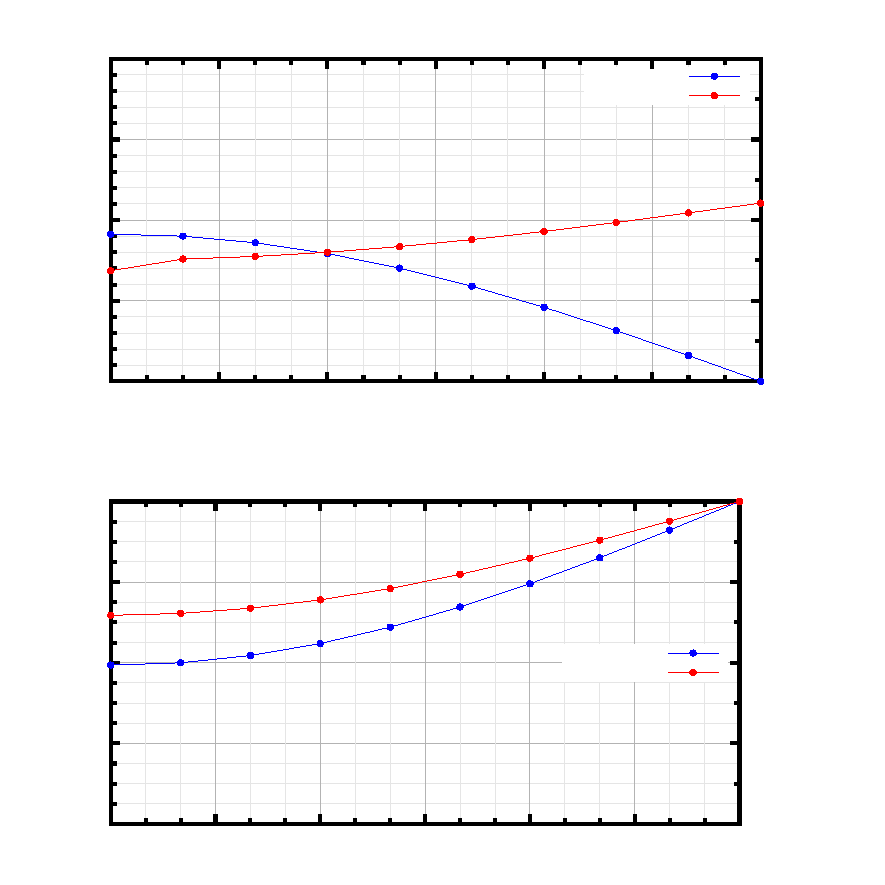
\includegraphics{../Code/11cTRAngle_Plot/11cTRAngle}}%
    \gplfronttext
  \end{picture}%
\endgroup
}
\caption{Maximum and minimum output voltage as well as a sweep of $v_\mathit{in}$ showing its affect on $V_\mathit{DS}$.}
\label{fig:11cTRAngle}
\end{center}
\end{figure}
\lstinputlisting{../Code/11cTRAngle_Plot/11cTRAngle_Plot.plt}

\section{Logscale On x-Axis (FFT)}
\begin{figure}[!htbp]
\begin{center}
\resizebox{\columnwidth}{!}{% GNUPLOT: LaTeX picture with Postscript
\begingroup
  \makeatletter
  \providecommand\color[2][]{%
    \GenericError{(gnuplot) \space\space\space\@spaces}{%
      Package color not loaded in conjunction with
      terminal option `colourtext'%
    }{See the gnuplot documentation for explanation.%
    }{Either use 'blacktext' in gnuplot or load the package
      color.sty in LaTeX.}%
    \renewcommand\color[2][]{}%
  }%
  \providecommand\includegraphics[2][]{%
    \GenericError{(gnuplot) \space\space\space\@spaces}{%
      Package graphicx or graphics not loaded%
    }{See the gnuplot documentation for explanation.%
    }{The gnuplot epslatex terminal needs graphicx.sty or graphics.sty.}%
    \renewcommand\includegraphics[2][]{}%
  }%
  \providecommand\rotatebox[2]{#2}%
  \@ifundefined{ifGPcolor}{%
    \newif\ifGPcolor
    \GPcolortrue
  }{}%
  \@ifundefined{ifGPblacktext}{%
    \newif\ifGPblacktext
    \GPblacktexttrue
  }{}%
  % define a \g@addto@macro without @ in the name:
  \let\gplgaddtomacro\g@addto@macro
  % define empty templates for all commands taking text:
  \gdef\gplbacktext{}%
  \gdef\gplfronttext{}%
  \makeatother
  \ifGPblacktext
    % no textcolor at all
    \def\colorrgb#1{}%
    \def\colorgray#1{}%
  \else
    % gray or color?
    \ifGPcolor
      \def\colorrgb#1{\color[rgb]{#1}}%
      \def\colorgray#1{\color[gray]{#1}}%
      \expandafter\def\csname LTw\endcsname{\color{white}}%
      \expandafter\def\csname LTb\endcsname{\color{black}}%
      \expandafter\def\csname LTa\endcsname{\color{black}}%
      \expandafter\def\csname LT0\endcsname{\color[rgb]{1,0,0}}%
      \expandafter\def\csname LT1\endcsname{\color[rgb]{0,1,0}}%
      \expandafter\def\csname LT2\endcsname{\color[rgb]{0,0,1}}%
      \expandafter\def\csname LT3\endcsname{\color[rgb]{1,0,1}}%
      \expandafter\def\csname LT4\endcsname{\color[rgb]{0,1,1}}%
      \expandafter\def\csname LT5\endcsname{\color[rgb]{1,1,0}}%
      \expandafter\def\csname LT6\endcsname{\color[rgb]{0,0,0}}%
      \expandafter\def\csname LT7\endcsname{\color[rgb]{1,0.3,0}}%
      \expandafter\def\csname LT8\endcsname{\color[rgb]{0.5,0.5,0.5}}%
    \else
      % gray
      \def\colorrgb#1{\color{black}}%
      \def\colorgray#1{\color[gray]{#1}}%
      \expandafter\def\csname LTw\endcsname{\color{white}}%
      \expandafter\def\csname LTb\endcsname{\color{black}}%
      \expandafter\def\csname LTa\endcsname{\color{black}}%
      \expandafter\def\csname LT0\endcsname{\color{black}}%
      \expandafter\def\csname LT1\endcsname{\color{black}}%
      \expandafter\def\csname LT2\endcsname{\color{black}}%
      \expandafter\def\csname LT3\endcsname{\color{black}}%
      \expandafter\def\csname LT4\endcsname{\color{black}}%
      \expandafter\def\csname LT5\endcsname{\color{black}}%
      \expandafter\def\csname LT6\endcsname{\color{black}}%
      \expandafter\def\csname LT7\endcsname{\color{black}}%
      \expandafter\def\csname LT8\endcsname{\color{black}}%
    \fi
  \fi
  \setlength{\unitlength}{0.0500bp}%
  \begin{picture}(8500.00,5660.00)%
    \gplgaddtomacro\gplbacktext{%
      \colorrgb{0.70,0.70,0.70}%
      \put(747,595){\makebox(0,0)[r]{\strut{}-160}}%
      \colorrgb{0.70,0.70,0.70}%
      \put(747,1096){\makebox(0,0)[r]{\strut{}-140}}%
      \colorrgb{0.70,0.70,0.70}%
      \put(747,1596){\makebox(0,0)[r]{\strut{}-120}}%
      \colorrgb{0.70,0.70,0.70}%
      \put(747,2097){\makebox(0,0)[r]{\strut{}-100}}%
      \colorrgb{0.70,0.70,0.70}%
      \put(747,2598){\makebox(0,0)[r]{\strut{}-80}}%
      \colorrgb{0.70,0.70,0.70}%
      \put(747,3098){\makebox(0,0)[r]{\strut{}-60}}%
      \colorrgb{0.70,0.70,0.70}%
      \put(747,3599){\makebox(0,0)[r]{\strut{}-40}}%
      \colorrgb{0.70,0.70,0.70}%
      \put(747,4100){\makebox(0,0)[r]{\strut{}-20}}%
      \colorrgb{0.70,0.70,0.70}%
      \put(747,4600){\makebox(0,0)[r]{\strut{} 0}}%
      \colorrgb{0.70,0.70,0.70}%
      \put(747,5101){\makebox(0,0)[r]{\strut{} 20}}%
      \colorrgb{0.70,0.70,0.70}%
      \put(849,409){\makebox(0,0){\strut{} 10}}%
      \colorrgb{0.70,0.70,0.70}%
      \put(3297,409){\makebox(0,0){\strut{} 100}}%
      \colorrgb{0.70,0.70,0.70}%
      \put(5745,409){\makebox(0,0){\strut{} 1000}}%
      \colorrgb{0.70,0.70,0.70}%
      \put(8193,409){\makebox(0,0){\strut{} 10000}}%
      \csname LTb\endcsname%
      \put(144,2848){\rotatebox{-270}{\makebox(0,0){\strut{}Output Voltage [dB]}}}%
      \csname LTb\endcsname%
      \put(4521,130){\makebox(0,0){\strut{}Frequency [Hz]}}%
      \put(4521,5380){\makebox(0,0){\strut{}Harmonic Distortion}}%
    }%
    \gplgaddtomacro\gplfronttext{%
    }%
    \gplbacktext
    \put(0,0){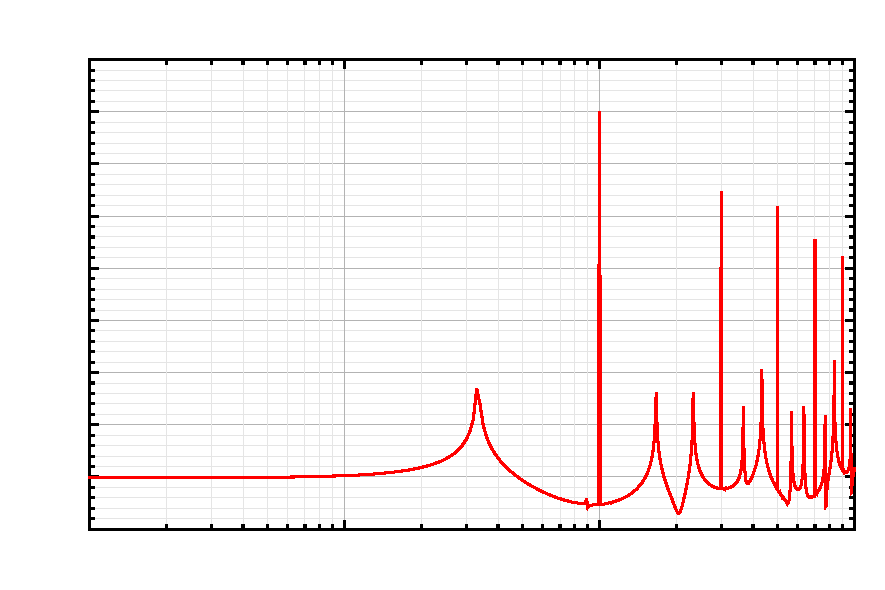
\includegraphics{../Code/FFT/FFT}}%
    \gplfronttext
  \end{picture}%
\endgroup
}
\caption{The x-scale is logarithmic and the y-axis is in decibel.}
\label{fig:FFT}
\end{center}
\end{figure}
\lstinputlisting{../Code/FFT/FFT.plt}

\section{Two Plots, Vertical Line Drawn And Coordinate Label}
\begin{figure}[!htbp]
\begin{center}
\resizebox{\columnwidth}{!}{% GNUPLOT: LaTeX picture with Postscript
\begingroup
  \makeatletter
  \providecommand\color[2][]{%
    \GenericError{(gnuplot) \space\space\space\@spaces}{%
      Package color not loaded in conjunction with
      terminal option `colourtext'%
    }{See the gnuplot documentation for explanation.%
    }{Either use 'blacktext' in gnuplot or load the package
      color.sty in LaTeX.}%
    \renewcommand\color[2][]{}%
  }%
  \providecommand\includegraphics[2][]{%
    \GenericError{(gnuplot) \space\space\space\@spaces}{%
      Package graphicx or graphics not loaded%
    }{See the gnuplot documentation for explanation.%
    }{The gnuplot epslatex terminal needs graphicx.sty or graphics.sty.}%
    \renewcommand\includegraphics[2][]{}%
  }%
  \providecommand\rotatebox[2]{#2}%
  \@ifundefined{ifGPcolor}{%
    \newif\ifGPcolor
    \GPcolortrue
  }{}%
  \@ifundefined{ifGPblacktext}{%
    \newif\ifGPblacktext
    \GPblacktexttrue
  }{}%
  % define a \g@addto@macro without @ in the name:
  \let\gplgaddtomacro\g@addto@macro
  % define empty templates for all commands taking text:
  \gdef\gplbacktext{}%
  \gdef\gplfronttext{}%
  \makeatother
  \ifGPblacktext
    % no textcolor at all
    \def\colorrgb#1{}%
    \def\colorgray#1{}%
  \else
    % gray or color?
    \ifGPcolor
      \def\colorrgb#1{\color[rgb]{#1}}%
      \def\colorgray#1{\color[gray]{#1}}%
      \expandafter\def\csname LTw\endcsname{\color{white}}%
      \expandafter\def\csname LTb\endcsname{\color{black}}%
      \expandafter\def\csname LTa\endcsname{\color{black}}%
      \expandafter\def\csname LT0\endcsname{\color[rgb]{1,0,0}}%
      \expandafter\def\csname LT1\endcsname{\color[rgb]{0,1,0}}%
      \expandafter\def\csname LT2\endcsname{\color[rgb]{0,0,1}}%
      \expandafter\def\csname LT3\endcsname{\color[rgb]{1,0,1}}%
      \expandafter\def\csname LT4\endcsname{\color[rgb]{0,1,1}}%
      \expandafter\def\csname LT5\endcsname{\color[rgb]{1,1,0}}%
      \expandafter\def\csname LT6\endcsname{\color[rgb]{0,0,0}}%
      \expandafter\def\csname LT7\endcsname{\color[rgb]{1,0.3,0}}%
      \expandafter\def\csname LT8\endcsname{\color[rgb]{0.5,0.5,0.5}}%
    \else
      % gray
      \def\colorrgb#1{\color{black}}%
      \def\colorgray#1{\color[gray]{#1}}%
      \expandafter\def\csname LTw\endcsname{\color{white}}%
      \expandafter\def\csname LTb\endcsname{\color{black}}%
      \expandafter\def\csname LTa\endcsname{\color{black}}%
      \expandafter\def\csname LT0\endcsname{\color{black}}%
      \expandafter\def\csname LT1\endcsname{\color{black}}%
      \expandafter\def\csname LT2\endcsname{\color{black}}%
      \expandafter\def\csname LT3\endcsname{\color{black}}%
      \expandafter\def\csname LT4\endcsname{\color{black}}%
      \expandafter\def\csname LT5\endcsname{\color{black}}%
      \expandafter\def\csname LT6\endcsname{\color{black}}%
      \expandafter\def\csname LT7\endcsname{\color{black}}%
      \expandafter\def\csname LT8\endcsname{\color{black}}%
    \fi
  \fi
  \setlength{\unitlength}{0.0500bp}%
  \begin{picture}(8500.00,8500.00)%
    \gplgaddtomacro\gplbacktext{%
      \colorrgb{0.70,0.70,0.70}%
      \put(543,4845){\makebox(0,0)[r]{\strut{}-3}}%
      \colorrgb{0.70,0.70,0.70}%
      \put(543,5361){\makebox(0,0)[r]{\strut{}-2}}%
      \colorrgb{0.70,0.70,0.70}%
      \put(543,5877){\makebox(0,0)[r]{\strut{}-1}}%
      \colorrgb{0.70,0.70,0.70}%
      \put(543,6393){\makebox(0,0)[r]{\strut{} 0}}%
      \colorrgb{0.70,0.70,0.70}%
      \put(543,6909){\makebox(0,0)[r]{\strut{} 1}}%
      \colorrgb{0.70,0.70,0.70}%
      \put(543,7425){\makebox(0,0)[r]{\strut{} 2}}%
      \colorrgb{0.70,0.70,0.70}%
      \put(543,7941){\makebox(0,0)[r]{\strut{} 3}}%
      \colorrgb{0.70,0.70,0.70}%
      \put(645,4659){\makebox(0,0){\strut{} 0}}%
      \colorrgb{0.70,0.70,0.70}%
      \put(1589,4659){\makebox(0,0){\strut{} 0.5}}%
      \colorrgb{0.70,0.70,0.70}%
      \put(2532,4659){\makebox(0,0){\strut{} 1}}%
      \colorrgb{0.70,0.70,0.70}%
      \put(3476,4659){\makebox(0,0){\strut{} 1.5}}%
      \colorrgb{0.70,0.70,0.70}%
      \put(4419,4659){\makebox(0,0){\strut{} 2}}%
      \colorrgb{0.70,0.70,0.70}%
      \put(5363,4659){\makebox(0,0){\strut{} 2.5}}%
      \colorrgb{0.70,0.70,0.70}%
      \put(6306,4659){\makebox(0,0){\strut{} 3}}%
      \colorrgb{0.70,0.70,0.70}%
      \put(7250,4659){\makebox(0,0){\strut{} 3.5}}%
      \colorrgb{0.70,0.70,0.70}%
      \put(8193,4659){\makebox(0,0){\strut{} 4}}%
      \csname LTb\endcsname%
      \put(144,6393){\rotatebox{-270}{\makebox(0,0){\strut{}Output Voltage [V]}}}%
      \csname LTb\endcsname%
      \put(4419,4380){\makebox(0,0){\strut{}Time [ms]}}%
      \put(4419,8220){\makebox(0,0){\strut{}Maximum And Minimum Output Voltage}}%
    }%
    \gplgaddtomacro\gplfronttext{%
    }%
    \gplgaddtomacro\gplbacktext{%
      \colorrgb{0.70,0.70,0.70}%
      \put(747,595){\makebox(0,0)[r]{\strut{} 0}}%
      \colorrgb{0.70,0.70,0.70}%
      \put(747,1111){\makebox(0,0)[r]{\strut{} 0.5}}%
      \colorrgb{0.70,0.70,0.70}%
      \put(747,1627){\makebox(0,0)[r]{\strut{} 1}}%
      \colorrgb{0.70,0.70,0.70}%
      \put(747,2144){\makebox(0,0)[r]{\strut{} 1.5}}%
      \colorrgb{0.70,0.70,0.70}%
      \put(747,2660){\makebox(0,0)[r]{\strut{} 2}}%
      \colorrgb{0.70,0.70,0.70}%
      \put(747,3176){\makebox(0,0)[r]{\strut{} 2.5}}%
      \colorrgb{0.70,0.70,0.70}%
      \put(747,3692){\makebox(0,0)[r]{\strut{} 3}}%
      \colorrgb{0.70,0.70,0.70}%
      \put(849,409){\makebox(0,0){\strut{} 0}}%
      \colorrgb{0.70,0.70,0.70}%
      \put(1583,409){\makebox(0,0){\strut{} 1}}%
      \colorrgb{0.70,0.70,0.70}%
      \put(2318,409){\makebox(0,0){\strut{} 2}}%
      \colorrgb{0.70,0.70,0.70}%
      \put(3052,409){\makebox(0,0){\strut{} 3}}%
      \colorrgb{0.70,0.70,0.70}%
      \put(3787,409){\makebox(0,0){\strut{} 4}}%
      \colorrgb{0.70,0.70,0.70}%
      \put(4521,409){\makebox(0,0){\strut{} 5}}%
      \colorrgb{0.70,0.70,0.70}%
      \put(5255,409){\makebox(0,0){\strut{} 6}}%
      \colorrgb{0.70,0.70,0.70}%
      \put(5990,409){\makebox(0,0){\strut{} 7}}%
      \colorrgb{0.70,0.70,0.70}%
      \put(6724,409){\makebox(0,0){\strut{} 8}}%
      \colorrgb{0.70,0.70,0.70}%
      \put(7459,409){\makebox(0,0){\strut{} 9}}%
      \colorrgb{0.70,0.70,0.70}%
      \put(8193,409){\makebox(0,0){\strut{} 10}}%
      \csname LTb\endcsname%
      \put(144,2143){\rotatebox{-270}{\makebox(0,0){\strut{}Drain-Source Voltage Of $Q1$ [V]}}}%
      \csname LTb\endcsname%
      \put(4521,130){\makebox(0,0){\strut{}$v_\mathit{in}$ (Swept) [V]}}%
      \put(4521,3971){\makebox(0,0){\strut{}Drain-Source Voltage Of $Q1$ For A Swept Input}}%
    }%
    \gplgaddtomacro\gplfronttext{%
      \colorrgb{0.68,0.85,0.90}%
      \put(3571,1174){\makebox(0,0)[l]{\strut{}(3.56,0.4)}}%
    }%
    \gplbacktext
    \put(0,0){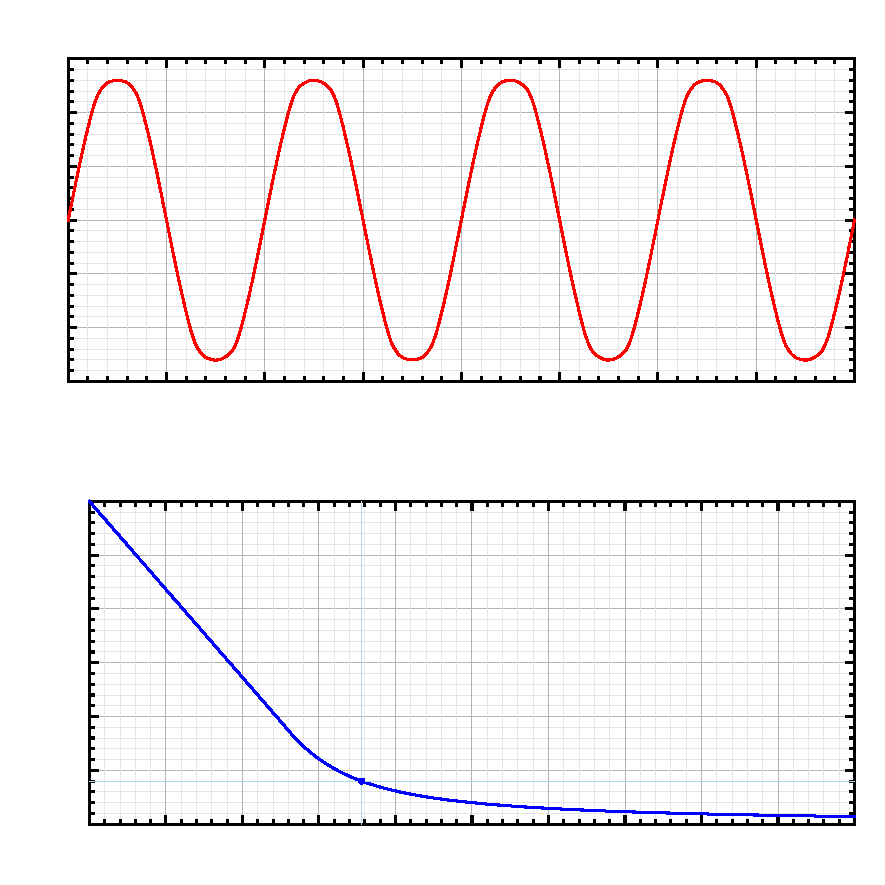
\includegraphics{../Code/MaxMinVoltages/MaxMinVoltages}}%
    \gplfronttext
  \end{picture}%
\endgroup
}
\caption{Maximum and minimum output voltage as well as a sweep of $v_\mathit{in}$ showing its affect on $V_\mathit{DS}$.}
\label{fig:MaxMinVoltages}
\end{center}
\end{figure}
\lstinputlisting{../Code/MaxMinVoltages/MaxMinVoltages.plt}

\section{Two Plots On The Same Plot And A Fit}
\begin{figure}[!hbtp]
\centering
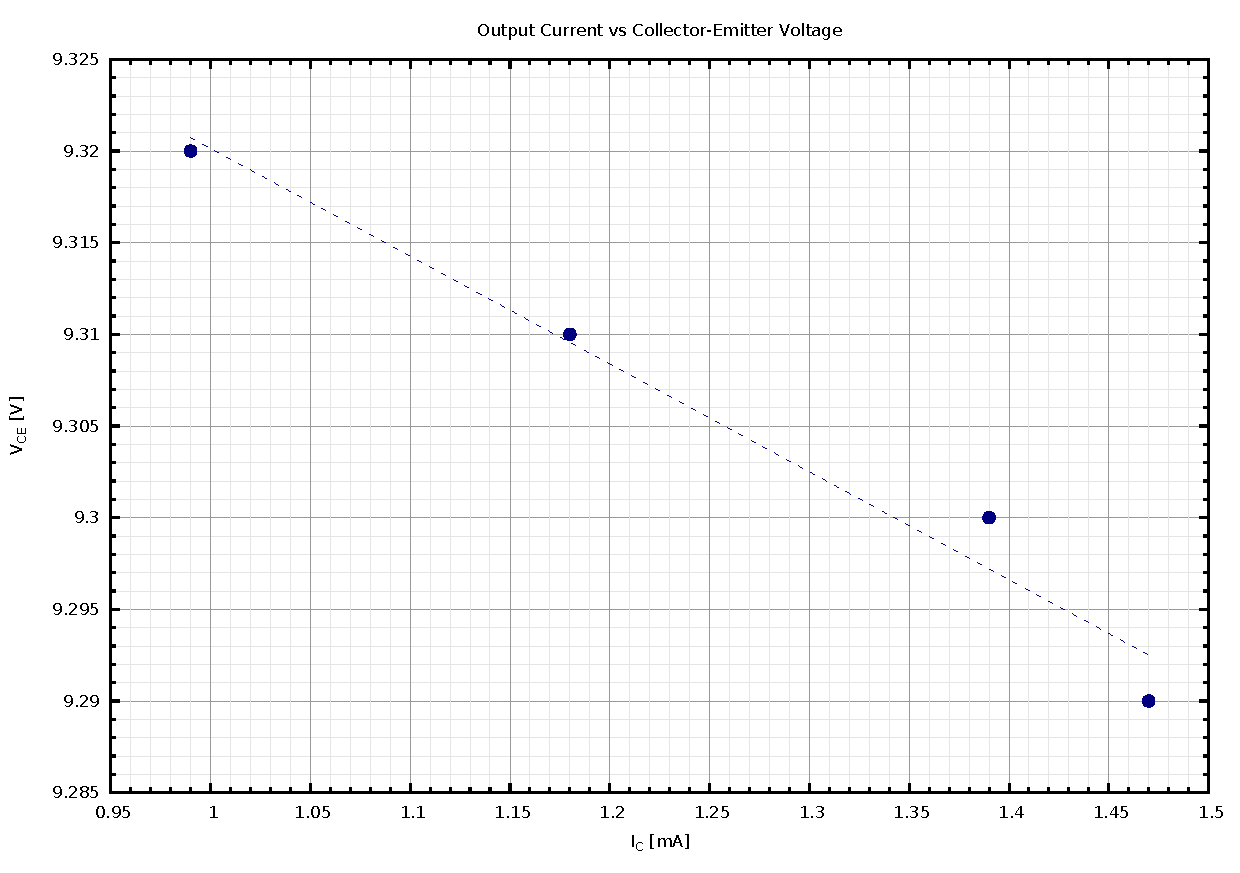
\includegraphics[width=\textwidth]{../Code/OutputResistanceQ2/OutputResistanceQ2.pdf}
\caption{Two plots on the same plot and a linear fit.}
\end{figure}
\lstinputlisting{../Code/OutputResistanceQ2/OutputResistanceQ2.plt}

\section{Thick Curves Do Not Exceed Frame And Major And Minor Gridlines Correctly Painted}
\begin{figure}[!hbtp]
\centering
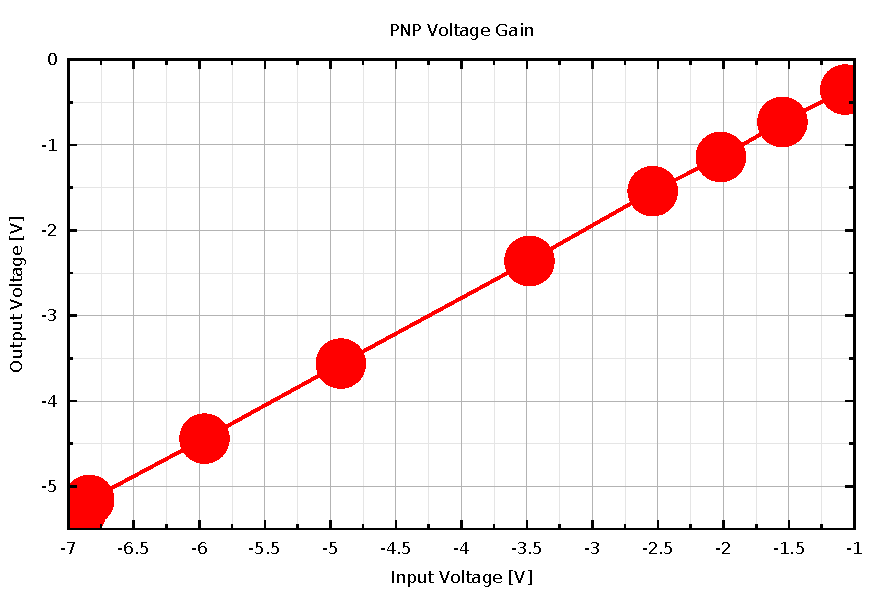
\includegraphics[width=\textwidth]{../Code/ElectronicCircuitsLab3/ElectronicCircuitsLab3.pdf}
\caption{Thick plots don't exceed the canvas's frame and the major and minor gridlines are correctly painted (major are drawn over the minor).}
\end{figure}
\lstinputlisting{../Code/ElectronicCircuitsLab3/ElectronicCircuitsLab3.plt}

\section{Multiple Data Plots}
\begin{figure}[!htbp]
\begin{center}
\resizebox{\columnwidth}{!}{% GNUPLOT: LaTeX picture with Postscript
\begingroup
  \makeatletter
  \providecommand\color[2][]{%
    \GenericError{(gnuplot) \space\space\space\@spaces}{%
      Package color not loaded in conjunction with
      terminal option `colourtext'%
    }{See the gnuplot documentation for explanation.%
    }{Either use 'blacktext' in gnuplot or load the package
      color.sty in LaTeX.}%
    \renewcommand\color[2][]{}%
  }%
  \providecommand\includegraphics[2][]{%
    \GenericError{(gnuplot) \space\space\space\@spaces}{%
      Package graphicx or graphics not loaded%
    }{See the gnuplot documentation for explanation.%
    }{The gnuplot epslatex terminal needs graphicx.sty or graphics.sty.}%
    \renewcommand\includegraphics[2][]{}%
  }%
  \providecommand\rotatebox[2]{#2}%
  \@ifundefined{ifGPcolor}{%
    \newif\ifGPcolor
    \GPcolortrue
  }{}%
  \@ifundefined{ifGPblacktext}{%
    \newif\ifGPblacktext
    \GPblacktexttrue
  }{}%
  % define a \g@addto@macro without @ in the name:
  \let\gplgaddtomacro\g@addto@macro
  % define empty templates for all commands taking text:
  \gdef\gplbacktext{}%
  \gdef\gplfronttext{}%
  \makeatother
  \ifGPblacktext
    % no textcolor at all
    \def\colorrgb#1{}%
    \def\colorgray#1{}%
  \else
    % gray or color?
    \ifGPcolor
      \def\colorrgb#1{\color[rgb]{#1}}%
      \def\colorgray#1{\color[gray]{#1}}%
      \expandafter\def\csname LTw\endcsname{\color{white}}%
      \expandafter\def\csname LTb\endcsname{\color{black}}%
      \expandafter\def\csname LTa\endcsname{\color{black}}%
      \expandafter\def\csname LT0\endcsname{\color[rgb]{1,0,0}}%
      \expandafter\def\csname LT1\endcsname{\color[rgb]{0,1,0}}%
      \expandafter\def\csname LT2\endcsname{\color[rgb]{0,0,1}}%
      \expandafter\def\csname LT3\endcsname{\color[rgb]{1,0,1}}%
      \expandafter\def\csname LT4\endcsname{\color[rgb]{0,1,1}}%
      \expandafter\def\csname LT5\endcsname{\color[rgb]{1,1,0}}%
      \expandafter\def\csname LT6\endcsname{\color[rgb]{0,0,0}}%
      \expandafter\def\csname LT7\endcsname{\color[rgb]{1,0.3,0}}%
      \expandafter\def\csname LT8\endcsname{\color[rgb]{0.5,0.5,0.5}}%
    \else
      % gray
      \def\colorrgb#1{\color{black}}%
      \def\colorgray#1{\color[gray]{#1}}%
      \expandafter\def\csname LTw\endcsname{\color{white}}%
      \expandafter\def\csname LTb\endcsname{\color{black}}%
      \expandafter\def\csname LTa\endcsname{\color{black}}%
      \expandafter\def\csname LT0\endcsname{\color{black}}%
      \expandafter\def\csname LT1\endcsname{\color{black}}%
      \expandafter\def\csname LT2\endcsname{\color{black}}%
      \expandafter\def\csname LT3\endcsname{\color{black}}%
      \expandafter\def\csname LT4\endcsname{\color{black}}%
      \expandafter\def\csname LT5\endcsname{\color{black}}%
      \expandafter\def\csname LT6\endcsname{\color{black}}%
      \expandafter\def\csname LT7\endcsname{\color{black}}%
      \expandafter\def\csname LT8\endcsname{\color{black}}%
    \fi
  \fi
  \setlength{\unitlength}{0.0500bp}%
  \begin{picture}(11320.00,14160.00)%
    \gplgaddtomacro\gplbacktext{%
      \colorrgb{0.60,0.60,0.60}%
      \put(645,11215){\makebox(0,0)[r]{\strut{}-4}}%
      \colorrgb{0.60,0.60,0.60}%
      \put(645,11556){\makebox(0,0)[r]{\strut{}-2}}%
      \colorrgb{0.60,0.60,0.60}%
      \put(645,11897){\makebox(0,0)[r]{\strut{} 0}}%
      \colorrgb{0.60,0.60,0.60}%
      \put(645,12238){\makebox(0,0)[r]{\strut{} 2}}%
      \colorrgb{0.60,0.60,0.60}%
      \put(645,12578){\makebox(0,0)[r]{\strut{} 4}}%
      \colorrgb{0.60,0.60,0.60}%
      \put(645,12919){\makebox(0,0)[r]{\strut{} 6}}%
      \colorrgb{0.60,0.60,0.60}%
      \put(645,13260){\makebox(0,0)[r]{\strut{} 8}}%
      \colorrgb{0.60,0.60,0.60}%
      \put(645,13601){\makebox(0,0)[r]{\strut{} 10}}%
      \colorrgb{0.60,0.60,0.60}%
      \put(747,11029){\makebox(0,0){\strut{} 0}}%
      \colorrgb{0.60,0.60,0.60}%
      \put(1515,11029){\makebox(0,0){\strut{} 0.5}}%
      \colorrgb{0.60,0.60,0.60}%
      \put(2282,11029){\makebox(0,0){\strut{} 1}}%
      \colorrgb{0.60,0.60,0.60}%
      \put(3050,11029){\makebox(0,0){\strut{} 1.5}}%
      \colorrgb{0.60,0.60,0.60}%
      \put(3818,11029){\makebox(0,0){\strut{} 2}}%
      \colorrgb{0.60,0.60,0.60}%
      \put(4585,11029){\makebox(0,0){\strut{} 2.5}}%
      \colorrgb{0.60,0.60,0.60}%
      \put(5353,11029){\makebox(0,0){\strut{} 3}}%
      \csname LTb\endcsname%
      \put(144,12408){\rotatebox{-270}{\makebox(0,0){\strut{}$v_a$ [V]}}}%
      \csname LTb\endcsname%
      \put(3050,10750){\makebox(0,0){\strut{}Time [s]}}%
      \put(3050,13880){\makebox(0,0){\strut{}Armature Voltage}}%
    }%
    \gplgaddtomacro\gplfronttext{%
    }%
    \gplgaddtomacro\gplbacktext{%
      \colorrgb{0.60,0.60,0.60}%
      \put(6407,11215){\makebox(0,0)[r]{\strut{}-0.1}}%
      \colorrgb{0.60,0.60,0.60}%
      \put(6407,11513){\makebox(0,0)[r]{\strut{} 0}}%
      \colorrgb{0.60,0.60,0.60}%
      \put(6407,11812){\makebox(0,0)[r]{\strut{} 0.1}}%
      \colorrgb{0.60,0.60,0.60}%
      \put(6407,12110){\makebox(0,0)[r]{\strut{} 0.2}}%
      \colorrgb{0.60,0.60,0.60}%
      \put(6407,12408){\makebox(0,0)[r]{\strut{} 0.3}}%
      \colorrgb{0.60,0.60,0.60}%
      \put(6407,12706){\makebox(0,0)[r]{\strut{} 0.4}}%
      \colorrgb{0.60,0.60,0.60}%
      \put(6407,13005){\makebox(0,0)[r]{\strut{} 0.5}}%
      \colorrgb{0.60,0.60,0.60}%
      \put(6407,13303){\makebox(0,0)[r]{\strut{} 0.6}}%
      \colorrgb{0.60,0.60,0.60}%
      \put(6407,13601){\makebox(0,0)[r]{\strut{} 0.7}}%
      \colorrgb{0.60,0.60,0.60}%
      \put(6509,11029){\makebox(0,0){\strut{} 0}}%
      \colorrgb{0.60,0.60,0.60}%
      \put(7260,11029){\makebox(0,0){\strut{} 0.5}}%
      \colorrgb{0.60,0.60,0.60}%
      \put(8010,11029){\makebox(0,0){\strut{} 1}}%
      \colorrgb{0.60,0.60,0.60}%
      \put(8761,11029){\makebox(0,0){\strut{} 1.5}}%
      \colorrgb{0.60,0.60,0.60}%
      \put(9512,11029){\makebox(0,0){\strut{} 2}}%
      \colorrgb{0.60,0.60,0.60}%
      \put(10262,11029){\makebox(0,0){\strut{} 2.5}}%
      \colorrgb{0.60,0.60,0.60}%
      \put(11013,11029){\makebox(0,0){\strut{} 3}}%
      \csname LTb\endcsname%
      \put(5804,12408){\rotatebox{-270}{\makebox(0,0){\strut{}$\theta_\mathit{opot}$ [\si{.\radian/\second}]}}}%
      \csname LTb\endcsname%
      \put(8761,10750){\makebox(0,0){\strut{}Time [s]}}%
      \put(8761,13880){\makebox(0,0){\strut{}Step Response ($\theta_\mathit{input}=0.5$)}}%
    }%
    \gplgaddtomacro\gplfronttext{%
    }%
    \gplgaddtomacro\gplbacktext{%
      \colorrgb{0.60,0.60,0.60}%
      \put(645,7675){\makebox(0,0)[r]{\strut{}-10}}%
      \colorrgb{0.60,0.60,0.60}%
      \put(645,8048){\makebox(0,0)[r]{\strut{}-5}}%
      \colorrgb{0.60,0.60,0.60}%
      \put(645,8421){\makebox(0,0)[r]{\strut{} 0}}%
      \colorrgb{0.60,0.60,0.60}%
      \put(645,8793){\makebox(0,0)[r]{\strut{} 5}}%
      \colorrgb{0.60,0.60,0.60}%
      \put(645,9166){\makebox(0,0)[r]{\strut{} 10}}%
      \colorrgb{0.60,0.60,0.60}%
      \put(645,9539){\makebox(0,0)[r]{\strut{} 15}}%
      \colorrgb{0.60,0.60,0.60}%
      \put(645,9912){\makebox(0,0)[r]{\strut{} 20}}%
      \colorrgb{0.60,0.60,0.60}%
      \put(747,7489){\makebox(0,0){\strut{} 0}}%
      \colorrgb{0.60,0.60,0.60}%
      \put(1515,7489){\makebox(0,0){\strut{} 0.5}}%
      \colorrgb{0.60,0.60,0.60}%
      \put(2282,7489){\makebox(0,0){\strut{} 1}}%
      \colorrgb{0.60,0.60,0.60}%
      \put(3050,7489){\makebox(0,0){\strut{} 1.5}}%
      \colorrgb{0.60,0.60,0.60}%
      \put(3818,7489){\makebox(0,0){\strut{} 2}}%
      \colorrgb{0.60,0.60,0.60}%
      \put(4585,7489){\makebox(0,0){\strut{} 2.5}}%
      \colorrgb{0.60,0.60,0.60}%
      \put(5353,7489){\makebox(0,0){\strut{} 3}}%
      \csname LTb\endcsname%
      \put(144,8868){\rotatebox{-270}{\makebox(0,0){\strut{}$v_a$ [V]}}}%
      \csname LTb\endcsname%
      \put(3050,7210){\makebox(0,0){\strut{}Time [s]}}%
      \put(3050,10340){\makebox(0,0){\strut{}Armature Voltage}}%
    }%
    \gplgaddtomacro\gplfronttext{%
    }%
    \gplgaddtomacro\gplbacktext{%
      \colorrgb{0.60,0.60,0.60}%
      \put(6407,7763){\makebox(0,0)[r]{\strut{} 0}}%
      \colorrgb{0.60,0.60,0.60}%
      \put(6407,8205){\makebox(0,0)[r]{\strut{} 0.5}}%
      \colorrgb{0.60,0.60,0.60}%
      \put(6407,8647){\makebox(0,0)[r]{\strut{} 1}}%
      \colorrgb{0.60,0.60,0.60}%
      \put(6407,9089){\makebox(0,0)[r]{\strut{} 1.5}}%
      \colorrgb{0.60,0.60,0.60}%
      \put(6407,9531){\makebox(0,0)[r]{\strut{} 2}}%
      \colorrgb{0.60,0.60,0.60}%
      \put(6407,9973){\makebox(0,0)[r]{\strut{} 2.5}}%
      \colorrgb{0.60,0.60,0.60}%
      \put(6509,7489){\makebox(0,0){\strut{} 0}}%
      \colorrgb{0.60,0.60,0.60}%
      \put(7260,7489){\makebox(0,0){\strut{} 0.5}}%
      \colorrgb{0.60,0.60,0.60}%
      \put(8010,7489){\makebox(0,0){\strut{} 1}}%
      \colorrgb{0.60,0.60,0.60}%
      \put(8761,7489){\makebox(0,0){\strut{} 1.5}}%
      \colorrgb{0.60,0.60,0.60}%
      \put(9512,7489){\makebox(0,0){\strut{} 2}}%
      \colorrgb{0.60,0.60,0.60}%
      \put(10262,7489){\makebox(0,0){\strut{} 2.5}}%
      \colorrgb{0.60,0.60,0.60}%
      \put(11013,7489){\makebox(0,0){\strut{} 3}}%
      \csname LTb\endcsname%
      \put(5804,8868){\rotatebox{-270}{\makebox(0,0){\strut{}$\theta_\mathit{opot}$ [\si{.\radian/\second}]}}}%
      \csname LTb\endcsname%
      \put(8761,7210){\makebox(0,0){\strut{}Time [s]}}%
      \put(8761,10340){\makebox(0,0){\strut{}Step Response ($\theta_\mathit{input}=2.0$)}}%
    }%
    \gplgaddtomacro\gplfronttext{%
    }%
    \gplgaddtomacro\gplbacktext{%
      \colorrgb{0.60,0.60,0.60}%
      \put(645,4334){\makebox(0,0)[r]{\strut{}-10}}%
      \colorrgb{0.60,0.60,0.60}%
      \put(645,4665){\makebox(0,0)[r]{\strut{}-5}}%
      \colorrgb{0.60,0.60,0.60}%
      \put(645,4997){\makebox(0,0)[r]{\strut{} 0}}%
      \colorrgb{0.60,0.60,0.60}%
      \put(645,5329){\makebox(0,0)[r]{\strut{} 5}}%
      \colorrgb{0.60,0.60,0.60}%
      \put(645,5660){\makebox(0,0)[r]{\strut{} 10}}%
      \colorrgb{0.60,0.60,0.60}%
      \put(645,5992){\makebox(0,0)[r]{\strut{} 15}}%
      \colorrgb{0.60,0.60,0.60}%
      \put(645,6323){\makebox(0,0)[r]{\strut{} 20}}%
      \colorrgb{0.60,0.60,0.60}%
      \put(747,3949){\makebox(0,0){\strut{} 0}}%
      \colorrgb{0.60,0.60,0.60}%
      \put(1515,3949){\makebox(0,0){\strut{} 0.5}}%
      \colorrgb{0.60,0.60,0.60}%
      \put(2282,3949){\makebox(0,0){\strut{} 1}}%
      \colorrgb{0.60,0.60,0.60}%
      \put(3050,3949){\makebox(0,0){\strut{} 1.5}}%
      \colorrgb{0.60,0.60,0.60}%
      \put(3818,3949){\makebox(0,0){\strut{} 2}}%
      \colorrgb{0.60,0.60,0.60}%
      \put(4585,3949){\makebox(0,0){\strut{} 2.5}}%
      \colorrgb{0.60,0.60,0.60}%
      \put(5353,3949){\makebox(0,0){\strut{} 3}}%
      \csname LTb\endcsname%
      \put(144,5328){\rotatebox{-270}{\makebox(0,0){\strut{}$v_a$ [V]}}}%
      \csname LTb\endcsname%
      \put(3050,3670){\makebox(0,0){\strut{}Time [s]}}%
      \put(3050,6801){\makebox(0,0){\strut{}Armature Voltage}}%
    }%
    \gplgaddtomacro\gplfronttext{%
    }%
    \gplgaddtomacro\gplbacktext{%
      \colorrgb{0.60,0.60,0.60}%
      \put(6203,4319){\makebox(0,0)[r]{\strut{} 0}}%
      \colorrgb{0.60,0.60,0.60}%
      \put(6203,4686){\makebox(0,0)[r]{\strut{} 1}}%
      \colorrgb{0.60,0.60,0.60}%
      \put(6203,5053){\makebox(0,0)[r]{\strut{} 2}}%
      \colorrgb{0.60,0.60,0.60}%
      \put(6203,5420){\makebox(0,0)[r]{\strut{} 3}}%
      \colorrgb{0.60,0.60,0.60}%
      \put(6203,5788){\makebox(0,0)[r]{\strut{} 4}}%
      \colorrgb{0.60,0.60,0.60}%
      \put(6203,6155){\makebox(0,0)[r]{\strut{} 5}}%
      \colorrgb{0.60,0.60,0.60}%
      \put(6203,6522){\makebox(0,0)[r]{\strut{} 6}}%
      \colorrgb{0.60,0.60,0.60}%
      \put(6305,3949){\makebox(0,0){\strut{} 0}}%
      \colorrgb{0.60,0.60,0.60}%
      \put(7090,3949){\makebox(0,0){\strut{} 0.5}}%
      \colorrgb{0.60,0.60,0.60}%
      \put(7874,3949){\makebox(0,0){\strut{} 1}}%
      \colorrgb{0.60,0.60,0.60}%
      \put(8659,3949){\makebox(0,0){\strut{} 1.5}}%
      \colorrgb{0.60,0.60,0.60}%
      \put(9444,3949){\makebox(0,0){\strut{} 2}}%
      \colorrgb{0.60,0.60,0.60}%
      \put(10228,3949){\makebox(0,0){\strut{} 2.5}}%
      \colorrgb{0.60,0.60,0.60}%
      \put(11013,3949){\makebox(0,0){\strut{} 3}}%
      \csname LTb\endcsname%
      \put(5804,5328){\rotatebox{-270}{\makebox(0,0){\strut{}$\theta_\mathit{opot}$ [\si{.\radian/\second}]}}}%
      \csname LTb\endcsname%
      \put(8659,3670){\makebox(0,0){\strut{}Time [s]}}%
      \put(8659,6801){\makebox(0,0){\strut{}Step Response ($\theta_\mathit{input}=5.0$)}}%
    }%
    \gplgaddtomacro\gplfronttext{%
    }%
    \gplgaddtomacro\gplbacktext{%
      \colorrgb{0.60,0.60,0.60}%
      \put(645,794){\makebox(0,0)[r]{\strut{}-10}}%
      \colorrgb{0.60,0.60,0.60}%
      \put(645,1125){\makebox(0,0)[r]{\strut{}-5}}%
      \colorrgb{0.60,0.60,0.60}%
      \put(645,1457){\makebox(0,0)[r]{\strut{} 0}}%
      \colorrgb{0.60,0.60,0.60}%
      \put(645,1789){\makebox(0,0)[r]{\strut{} 5}}%
      \colorrgb{0.60,0.60,0.60}%
      \put(645,2120){\makebox(0,0)[r]{\strut{} 10}}%
      \colorrgb{0.60,0.60,0.60}%
      \put(645,2452){\makebox(0,0)[r]{\strut{} 15}}%
      \colorrgb{0.60,0.60,0.60}%
      \put(645,2783){\makebox(0,0)[r]{\strut{} 20}}%
      \colorrgb{0.60,0.60,0.60}%
      \put(747,409){\makebox(0,0){\strut{} 0}}%
      \colorrgb{0.60,0.60,0.60}%
      \put(1515,409){\makebox(0,0){\strut{} 0.5}}%
      \colorrgb{0.60,0.60,0.60}%
      \put(2282,409){\makebox(0,0){\strut{} 1}}%
      \colorrgb{0.60,0.60,0.60}%
      \put(3050,409){\makebox(0,0){\strut{} 1.5}}%
      \colorrgb{0.60,0.60,0.60}%
      \put(3818,409){\makebox(0,0){\strut{} 2}}%
      \colorrgb{0.60,0.60,0.60}%
      \put(4585,409){\makebox(0,0){\strut{} 2.5}}%
      \colorrgb{0.60,0.60,0.60}%
      \put(5353,409){\makebox(0,0){\strut{} 3}}%
      \csname LTb\endcsname%
      \put(144,1788){\rotatebox{-270}{\makebox(0,0){\strut{}$v_a$ [V]}}}%
      \csname LTb\endcsname%
      \put(3050,130){\makebox(0,0){\strut{}Time [s]}}%
      \put(3050,3261){\makebox(0,0){\strut{}Armature Voltage}}%
    }%
    \gplgaddtomacro\gplfronttext{%
    }%
    \gplgaddtomacro\gplbacktext{%
      \colorrgb{0.60,0.60,0.60}%
      \put(6305,779){\makebox(0,0)[r]{\strut{} 0}}%
      \colorrgb{0.60,0.60,0.60}%
      \put(6305,1146){\makebox(0,0)[r]{\strut{} 2}}%
      \colorrgb{0.60,0.60,0.60}%
      \put(6305,1513){\makebox(0,0)[r]{\strut{} 4}}%
      \colorrgb{0.60,0.60,0.60}%
      \put(6305,1880){\makebox(0,0)[r]{\strut{} 6}}%
      \colorrgb{0.60,0.60,0.60}%
      \put(6305,2248){\makebox(0,0)[r]{\strut{} 8}}%
      \colorrgb{0.60,0.60,0.60}%
      \put(6305,2615){\makebox(0,0)[r]{\strut{} 10}}%
      \colorrgb{0.60,0.60,0.60}%
      \put(6305,2982){\makebox(0,0)[r]{\strut{} 12}}%
      \colorrgb{0.60,0.60,0.60}%
      \put(6407,409){\makebox(0,0){\strut{} 0}}%
      \colorrgb{0.60,0.60,0.60}%
      \put(7175,409){\makebox(0,0){\strut{} 0.5}}%
      \colorrgb{0.60,0.60,0.60}%
      \put(7942,409){\makebox(0,0){\strut{} 1}}%
      \colorrgb{0.60,0.60,0.60}%
      \put(8710,409){\makebox(0,0){\strut{} 1.5}}%
      \colorrgb{0.60,0.60,0.60}%
      \put(9478,409){\makebox(0,0){\strut{} 2}}%
      \colorrgb{0.60,0.60,0.60}%
      \put(10245,409){\makebox(0,0){\strut{} 2.5}}%
      \colorrgb{0.60,0.60,0.60}%
      \put(11013,409){\makebox(0,0){\strut{} 3}}%
      \csname LTb\endcsname%
      \put(5804,1788){\rotatebox{-270}{\makebox(0,0){\strut{}$\theta_\mathit{opot}$ [\si{.\radian/\second}]}}}%
      \csname LTb\endcsname%
      \put(8710,130){\makebox(0,0){\strut{}Time [s]}}%
      \put(8710,3261){\makebox(0,0){\strut{}Step Response ($\theta_\mathit{input}=10$)}}%
    }%
    \gplgaddtomacro\gplfronttext{%
    }%
    \gplbacktext
    \put(0,0){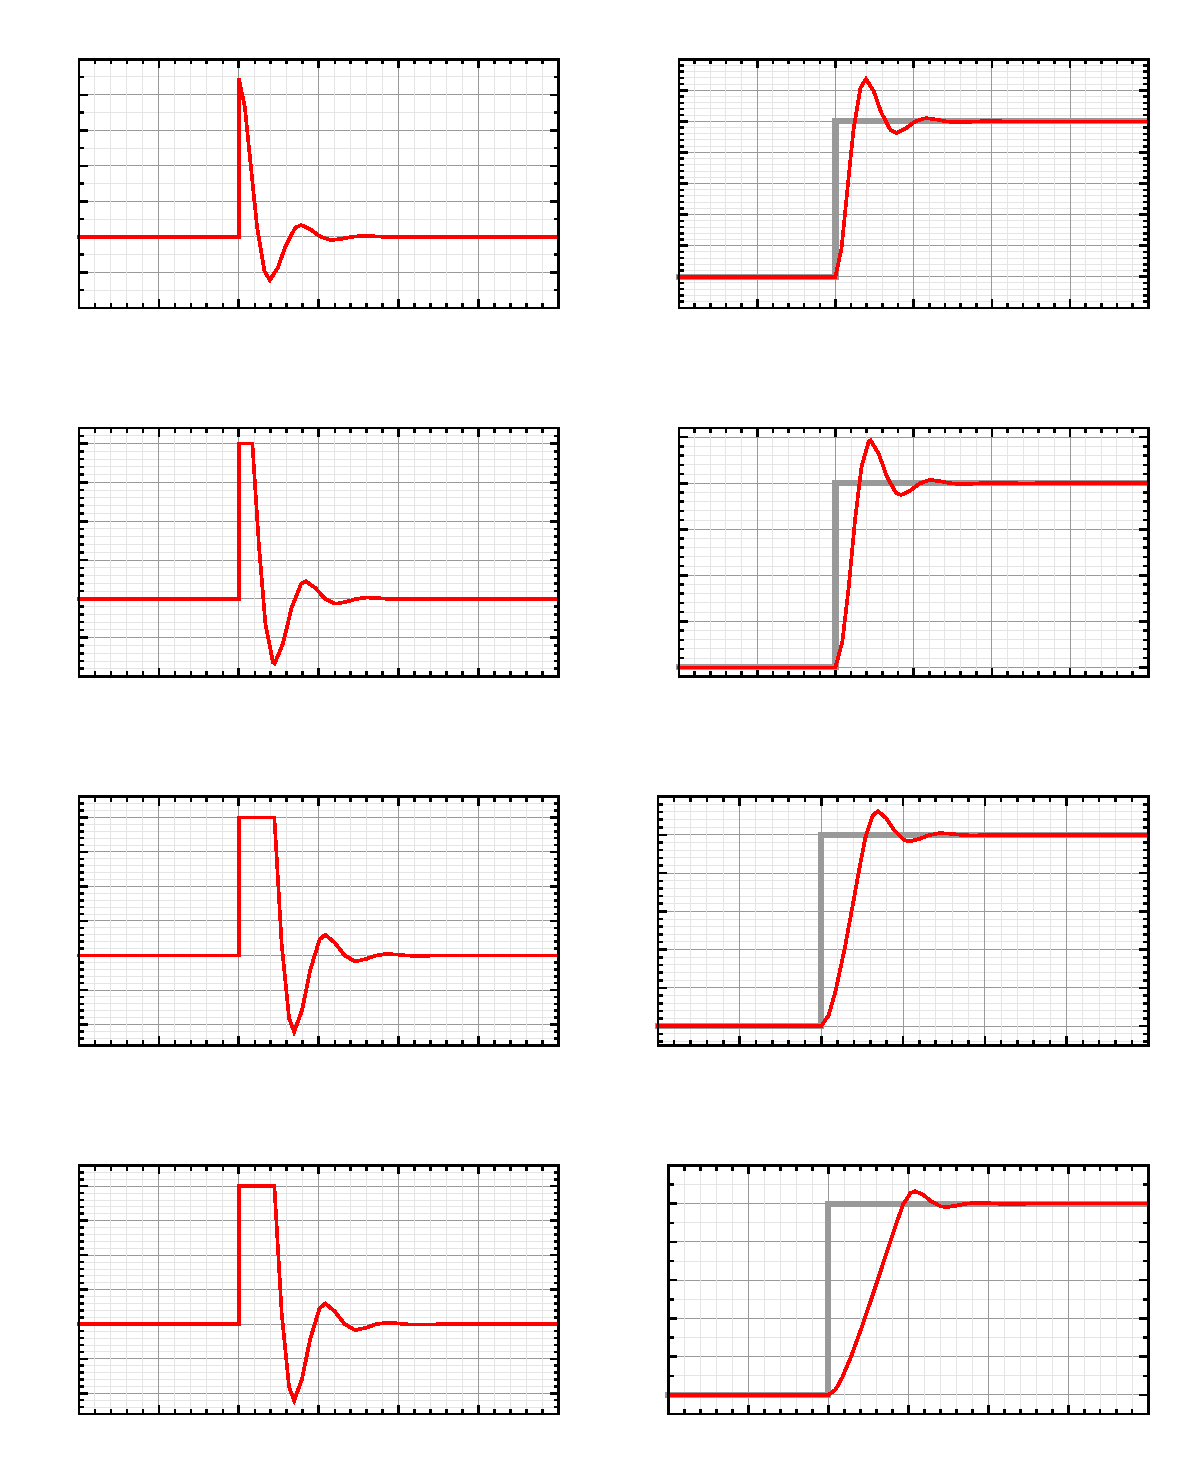
\includegraphics{../Code/Motor/Motor}}%
    \gplfronttext
  \end{picture}%
\endgroup
}
\caption{Multiple data files plotted onto a page and \LaTeX fonts.}
\label{fig:Motor}
\end{center}
\end{figure}
\lstinputlisting{../Code/Motor/Motor.plt}


\section{TikZ Terminal, Transparent Fille, Correct Gridlines And Curve Does Not Exceed Canvas}
\begin{figure}[htbp]
\begin{center}
\resizebox{\columnwidth}{!}{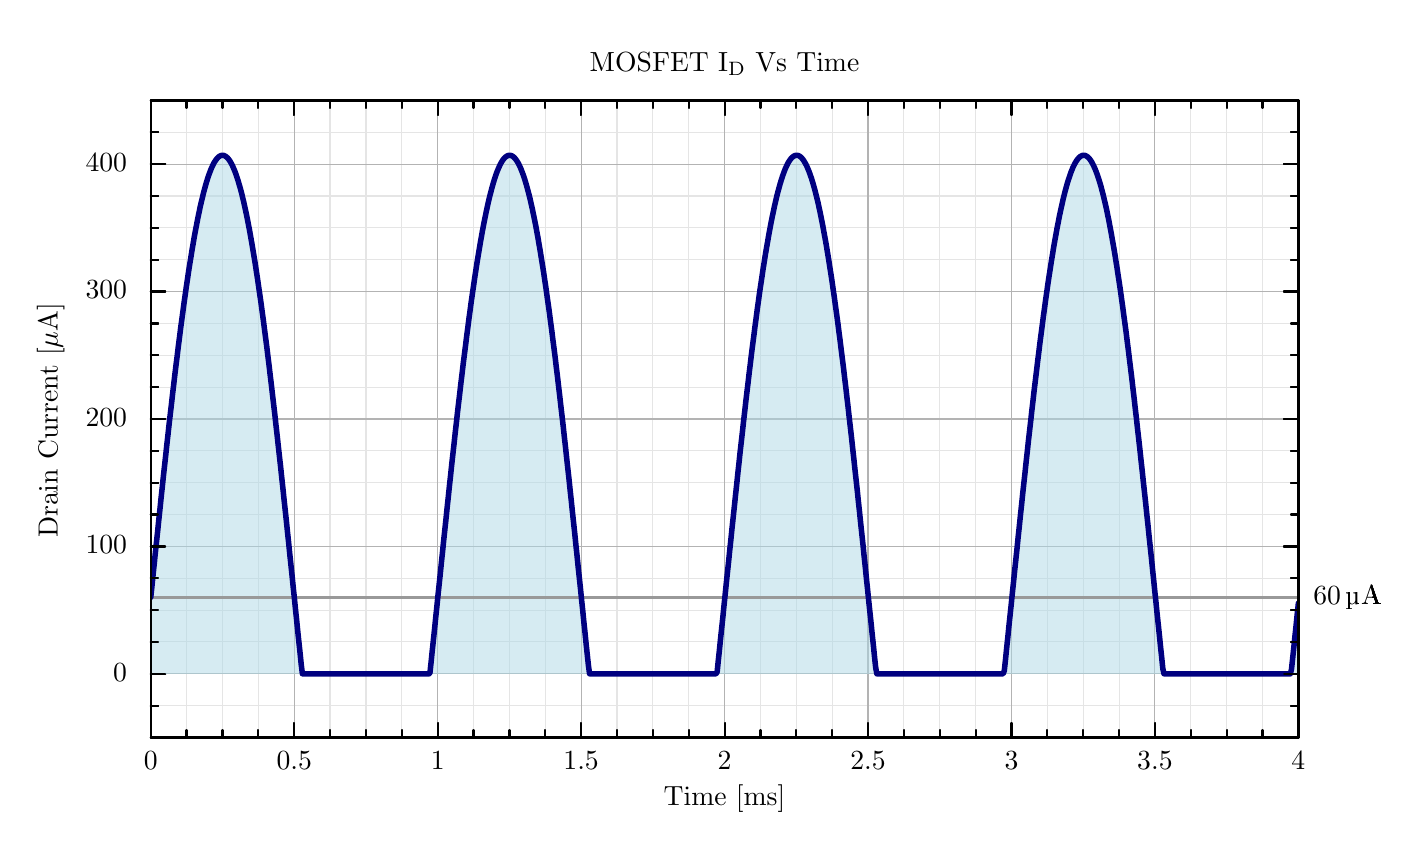
\begin{tikzpicture}[gnuplot]
%% generated with GNUPLOT 4.6p1 (Lua 5.1; terminal rev. 99, script rev. 100)
%% Sun 06 Oct 2013 03:10:49 EST
\path (0.000,0.000) rectangle (17.000,10.000);
\gpfill{color=gpbgfillcolor} (0.000,0.000)--(1.504,0.000)--(1.504,9.999)--(0.000,9.999)--cycle;
\gpfill{color=gpbgfillcolor} (16.079,0.000)--(16.999,0.000)--(16.999,9.999)--(16.079,9.999)--cycle;
\gpfill{color=gpbgfillcolor} (0.000,9.075)--(16.999,9.075)--(16.999,9.999)--(0.000,9.999)--cycle;
\gpfill{color=gpbgfillcolor} (0.000,0.000)--(16.999,0.000)--(16.999,0.985)--(0.000,0.985)--cycle;
\gpcolor{rgb color={0.898,0.898,0.898}}
\gpsetlinetype{gp lt border}
\gpsetlinewidth{1.00}
\draw[gp path] (1.504,0.985)--(16.079,0.985);
\gpcolor{color=gp lt color border}
\gpsetlinewidth{2.00}
\draw[gp path] (1.504,0.985)--(1.594,0.985);
\draw[gp path] (16.079,0.985)--(15.989,0.985);
\gpcolor{rgb color={0.898,0.898,0.898}}
\gpsetlinewidth{1.00}
\draw[gp path] (1.504,1.390)--(16.079,1.390);
\gpcolor{color=gp lt color border}
\gpsetlinewidth{2.00}
\draw[gp path] (1.504,1.390)--(1.594,1.390);
\draw[gp path] (16.079,1.390)--(15.989,1.390);
\draw[gp path] (1.504,1.794)--(1.684,1.794);
\draw[gp path] (16.079,1.794)--(15.899,1.794);
\node[gp node right] at (1.320,1.794) { 0};
\gpcolor{rgb color={0.898,0.898,0.898}}
\gpsetlinewidth{1.00}
\draw[gp path] (1.504,2.199)--(16.079,2.199);
\gpcolor{color=gp lt color border}
\gpsetlinewidth{2.00}
\draw[gp path] (1.504,2.199)--(1.594,2.199);
\draw[gp path] (16.079,2.199)--(15.989,2.199);
\gpcolor{rgb color={0.898,0.898,0.898}}
\gpsetlinewidth{1.00}
\draw[gp path] (1.504,2.603)--(16.079,2.603);
\gpcolor{color=gp lt color border}
\gpsetlinewidth{2.00}
\draw[gp path] (1.504,2.603)--(1.594,2.603);
\draw[gp path] (16.079,2.603)--(15.989,2.603);
\gpcolor{rgb color={0.898,0.898,0.898}}
\gpsetlinewidth{1.00}
\draw[gp path] (1.504,3.008)--(16.079,3.008);
\gpcolor{color=gp lt color border}
\gpsetlinewidth{2.00}
\draw[gp path] (1.504,3.008)--(1.594,3.008);
\draw[gp path] (16.079,3.008)--(15.989,3.008);
\draw[gp path] (1.504,3.412)--(1.684,3.412);
\draw[gp path] (16.079,3.412)--(15.899,3.412);
\node[gp node right] at (1.320,3.412) { 100};
\gpcolor{rgb color={0.898,0.898,0.898}}
\gpsetlinewidth{1.00}
\draw[gp path] (1.504,3.817)--(16.079,3.817);
\gpcolor{color=gp lt color border}
\gpsetlinewidth{2.00}
\draw[gp path] (1.504,3.817)--(1.594,3.817);
\draw[gp path] (16.079,3.817)--(15.989,3.817);
\gpcolor{rgb color={0.898,0.898,0.898}}
\gpsetlinewidth{1.00}
\draw[gp path] (1.504,4.221)--(16.079,4.221);
\gpcolor{color=gp lt color border}
\gpsetlinewidth{2.00}
\draw[gp path] (1.504,4.221)--(1.594,4.221);
\draw[gp path] (16.079,4.221)--(15.989,4.221);
\gpcolor{rgb color={0.898,0.898,0.898}}
\gpsetlinewidth{1.00}
\draw[gp path] (1.504,4.626)--(16.079,4.626);
\gpcolor{color=gp lt color border}
\gpsetlinewidth{2.00}
\draw[gp path] (1.504,4.626)--(1.594,4.626);
\draw[gp path] (16.079,4.626)--(15.989,4.626);
\draw[gp path] (1.504,5.030)--(1.684,5.030);
\draw[gp path] (16.079,5.030)--(15.899,5.030);
\node[gp node right] at (1.320,5.030) { 200};
\gpcolor{rgb color={0.898,0.898,0.898}}
\gpsetlinewidth{1.00}
\draw[gp path] (1.504,5.435)--(16.079,5.435);
\gpcolor{color=gp lt color border}
\gpsetlinewidth{2.00}
\draw[gp path] (1.504,5.435)--(1.594,5.435);
\draw[gp path] (16.079,5.435)--(15.989,5.435);
\gpcolor{rgb color={0.898,0.898,0.898}}
\gpsetlinewidth{1.00}
\draw[gp path] (1.504,5.839)--(16.079,5.839);
\gpcolor{color=gp lt color border}
\gpsetlinewidth{2.00}
\draw[gp path] (1.504,5.839)--(1.594,5.839);
\draw[gp path] (16.079,5.839)--(15.989,5.839);
\gpcolor{rgb color={0.898,0.898,0.898}}
\gpsetlinewidth{1.00}
\draw[gp path] (1.504,6.244)--(16.079,6.244);
\gpcolor{color=gp lt color border}
\gpsetlinewidth{2.00}
\draw[gp path] (1.504,6.244)--(1.594,6.244);
\draw[gp path] (16.079,6.244)--(15.989,6.244);
\draw[gp path] (1.504,6.648)--(1.684,6.648);
\draw[gp path] (16.079,6.648)--(15.899,6.648);
\node[gp node right] at (1.320,6.648) { 300};
\gpcolor{rgb color={0.898,0.898,0.898}}
\gpsetlinewidth{1.00}
\draw[gp path] (1.504,7.053)--(16.079,7.053);
\gpcolor{color=gp lt color border}
\gpsetlinewidth{2.00}
\draw[gp path] (1.504,7.053)--(1.594,7.053);
\draw[gp path] (16.079,7.053)--(15.989,7.053);
\gpcolor{rgb color={0.898,0.898,0.898}}
\gpsetlinewidth{1.00}
\draw[gp path] (1.504,7.457)--(16.079,7.457);
\gpcolor{color=gp lt color border}
\gpsetlinewidth{2.00}
\draw[gp path] (1.504,7.457)--(1.594,7.457);
\draw[gp path] (16.079,7.457)--(15.989,7.457);
\gpcolor{rgb color={0.898,0.898,0.898}}
\gpsetlinewidth{1.00}
\draw[gp path] (1.504,7.862)--(16.079,7.862);
\gpcolor{color=gp lt color border}
\gpsetlinewidth{2.00}
\draw[gp path] (1.504,7.862)--(1.594,7.862);
\draw[gp path] (16.079,7.862)--(15.989,7.862);
\draw[gp path] (1.504,8.266)--(1.684,8.266);
\draw[gp path] (16.079,8.266)--(15.899,8.266);
\node[gp node right] at (1.320,8.266) { 400};
\gpcolor{rgb color={0.898,0.898,0.898}}
\gpsetlinewidth{1.00}
\draw[gp path] (1.504,8.671)--(16.079,8.671);
\gpcolor{color=gp lt color border}
\gpsetlinewidth{2.00}
\draw[gp path] (1.504,8.671)--(1.594,8.671);
\draw[gp path] (16.079,8.671)--(15.989,8.671);
\gpcolor{rgb color={0.898,0.898,0.898}}
\gpsetlinewidth{1.00}
\draw[gp path] (1.504,9.075)--(16.079,9.075);
\gpcolor{color=gp lt color border}
\gpsetlinewidth{2.00}
\draw[gp path] (1.504,9.075)--(1.594,9.075);
\draw[gp path] (16.079,9.075)--(15.989,9.075);
\draw[gp path] (1.504,0.985)--(1.504,1.165);
\draw[gp path] (1.504,9.075)--(1.504,8.895);
\node[gp node center] at (1.504,0.677) { 0};
\gpcolor{rgb color={0.898,0.898,0.898}}
\gpsetlinewidth{1.00}
\draw[gp path] (1.959,0.985)--(1.959,9.075);
\gpcolor{color=gp lt color border}
\gpsetlinewidth{2.00}
\draw[gp path] (1.959,0.985)--(1.959,1.075);
\draw[gp path] (1.959,9.075)--(1.959,8.985);
\gpcolor{rgb color={0.898,0.898,0.898}}
\gpsetlinewidth{1.00}
\draw[gp path] (2.415,0.985)--(2.415,9.075);
\gpcolor{color=gp lt color border}
\gpsetlinewidth{2.00}
\draw[gp path] (2.415,0.985)--(2.415,1.075);
\draw[gp path] (2.415,9.075)--(2.415,8.985);
\gpcolor{rgb color={0.898,0.898,0.898}}
\gpsetlinewidth{1.00}
\draw[gp path] (2.870,0.985)--(2.870,9.075);
\gpcolor{color=gp lt color border}
\gpsetlinewidth{2.00}
\draw[gp path] (2.870,0.985)--(2.870,1.075);
\draw[gp path] (2.870,9.075)--(2.870,8.985);
\draw[gp path] (3.326,0.985)--(3.326,1.165);
\draw[gp path] (3.326,9.075)--(3.326,8.895);
\node[gp node center] at (3.326,0.677) { 0.5};
\gpcolor{rgb color={0.898,0.898,0.898}}
\gpsetlinewidth{1.00}
\draw[gp path] (3.781,0.985)--(3.781,9.075);
\gpcolor{color=gp lt color border}
\gpsetlinewidth{2.00}
\draw[gp path] (3.781,0.985)--(3.781,1.075);
\draw[gp path] (3.781,9.075)--(3.781,8.985);
\gpcolor{rgb color={0.898,0.898,0.898}}
\gpsetlinewidth{1.00}
\draw[gp path] (4.237,0.985)--(4.237,9.075);
\gpcolor{color=gp lt color border}
\gpsetlinewidth{2.00}
\draw[gp path] (4.237,0.985)--(4.237,1.075);
\draw[gp path] (4.237,9.075)--(4.237,8.985);
\gpcolor{rgb color={0.898,0.898,0.898}}
\gpsetlinewidth{1.00}
\draw[gp path] (4.692,0.985)--(4.692,9.075);
\gpcolor{color=gp lt color border}
\gpsetlinewidth{2.00}
\draw[gp path] (4.692,0.985)--(4.692,1.075);
\draw[gp path] (4.692,9.075)--(4.692,8.985);
\draw[gp path] (5.148,0.985)--(5.148,1.165);
\draw[gp path] (5.148,9.075)--(5.148,8.895);
\node[gp node center] at (5.148,0.677) { 1};
\gpcolor{rgb color={0.898,0.898,0.898}}
\gpsetlinewidth{1.00}
\draw[gp path] (5.603,0.985)--(5.603,9.075);
\gpcolor{color=gp lt color border}
\gpsetlinewidth{2.00}
\draw[gp path] (5.603,0.985)--(5.603,1.075);
\draw[gp path] (5.603,9.075)--(5.603,8.985);
\gpcolor{rgb color={0.898,0.898,0.898}}
\gpsetlinewidth{1.00}
\draw[gp path] (6.059,0.985)--(6.059,9.075);
\gpcolor{color=gp lt color border}
\gpsetlinewidth{2.00}
\draw[gp path] (6.059,0.985)--(6.059,1.075);
\draw[gp path] (6.059,9.075)--(6.059,8.985);
\gpcolor{rgb color={0.898,0.898,0.898}}
\gpsetlinewidth{1.00}
\draw[gp path] (6.514,0.985)--(6.514,9.075);
\gpcolor{color=gp lt color border}
\gpsetlinewidth{2.00}
\draw[gp path] (6.514,0.985)--(6.514,1.075);
\draw[gp path] (6.514,9.075)--(6.514,8.985);
\draw[gp path] (6.970,0.985)--(6.970,1.165);
\draw[gp path] (6.970,9.075)--(6.970,8.895);
\node[gp node center] at (6.970,0.677) { 1.5};
\gpcolor{rgb color={0.898,0.898,0.898}}
\gpsetlinewidth{1.00}
\draw[gp path] (7.425,0.985)--(7.425,9.075);
\gpcolor{color=gp lt color border}
\gpsetlinewidth{2.00}
\draw[gp path] (7.425,0.985)--(7.425,1.075);
\draw[gp path] (7.425,9.075)--(7.425,8.985);
\gpcolor{rgb color={0.898,0.898,0.898}}
\gpsetlinewidth{1.00}
\draw[gp path] (7.881,0.985)--(7.881,9.075);
\gpcolor{color=gp lt color border}
\gpsetlinewidth{2.00}
\draw[gp path] (7.881,0.985)--(7.881,1.075);
\draw[gp path] (7.881,9.075)--(7.881,8.985);
\gpcolor{rgb color={0.898,0.898,0.898}}
\gpsetlinewidth{1.00}
\draw[gp path] (8.336,0.985)--(8.336,9.075);
\gpcolor{color=gp lt color border}
\gpsetlinewidth{2.00}
\draw[gp path] (8.336,0.985)--(8.336,1.075);
\draw[gp path] (8.336,9.075)--(8.336,8.985);
\draw[gp path] (8.792,0.985)--(8.792,1.165);
\draw[gp path] (8.792,9.075)--(8.792,8.895);
\node[gp node center] at (8.792,0.677) { 2};
\gpcolor{rgb color={0.898,0.898,0.898}}
\gpsetlinewidth{1.00}
\draw[gp path] (9.247,0.985)--(9.247,9.075);
\gpcolor{color=gp lt color border}
\gpsetlinewidth{2.00}
\draw[gp path] (9.247,0.985)--(9.247,1.075);
\draw[gp path] (9.247,9.075)--(9.247,8.985);
\gpcolor{rgb color={0.898,0.898,0.898}}
\gpsetlinewidth{1.00}
\draw[gp path] (9.702,0.985)--(9.702,9.075);
\gpcolor{color=gp lt color border}
\gpsetlinewidth{2.00}
\draw[gp path] (9.702,0.985)--(9.702,1.075);
\draw[gp path] (9.702,9.075)--(9.702,8.985);
\gpcolor{rgb color={0.898,0.898,0.898}}
\gpsetlinewidth{1.00}
\draw[gp path] (10.158,0.985)--(10.158,9.075);
\gpcolor{color=gp lt color border}
\gpsetlinewidth{2.00}
\draw[gp path] (10.158,0.985)--(10.158,1.075);
\draw[gp path] (10.158,9.075)--(10.158,8.985);
\draw[gp path] (10.613,0.985)--(10.613,1.165);
\draw[gp path] (10.613,9.075)--(10.613,8.895);
\node[gp node center] at (10.613,0.677) { 2.5};
\gpcolor{rgb color={0.898,0.898,0.898}}
\gpsetlinewidth{1.00}
\draw[gp path] (11.069,0.985)--(11.069,9.075);
\gpcolor{color=gp lt color border}
\gpsetlinewidth{2.00}
\draw[gp path] (11.069,0.985)--(11.069,1.075);
\draw[gp path] (11.069,9.075)--(11.069,8.985);
\gpcolor{rgb color={0.898,0.898,0.898}}
\gpsetlinewidth{1.00}
\draw[gp path] (11.524,0.985)--(11.524,9.075);
\gpcolor{color=gp lt color border}
\gpsetlinewidth{2.00}
\draw[gp path] (11.524,0.985)--(11.524,1.075);
\draw[gp path] (11.524,9.075)--(11.524,8.985);
\gpcolor{rgb color={0.898,0.898,0.898}}
\gpsetlinewidth{1.00}
\draw[gp path] (11.980,0.985)--(11.980,9.075);
\gpcolor{color=gp lt color border}
\gpsetlinewidth{2.00}
\draw[gp path] (11.980,0.985)--(11.980,1.075);
\draw[gp path] (11.980,9.075)--(11.980,8.985);
\draw[gp path] (12.435,0.985)--(12.435,1.165);
\draw[gp path] (12.435,9.075)--(12.435,8.895);
\node[gp node center] at (12.435,0.677) { 3};
\gpcolor{rgb color={0.898,0.898,0.898}}
\gpsetlinewidth{1.00}
\draw[gp path] (12.891,0.985)--(12.891,9.075);
\gpcolor{color=gp lt color border}
\gpsetlinewidth{2.00}
\draw[gp path] (12.891,0.985)--(12.891,1.075);
\draw[gp path] (12.891,9.075)--(12.891,8.985);
\gpcolor{rgb color={0.898,0.898,0.898}}
\gpsetlinewidth{1.00}
\draw[gp path] (13.346,0.985)--(13.346,9.075);
\gpcolor{color=gp lt color border}
\gpsetlinewidth{2.00}
\draw[gp path] (13.346,0.985)--(13.346,1.075);
\draw[gp path] (13.346,9.075)--(13.346,8.985);
\gpcolor{rgb color={0.898,0.898,0.898}}
\gpsetlinewidth{1.00}
\draw[gp path] (13.802,0.985)--(13.802,9.075);
\gpcolor{color=gp lt color border}
\gpsetlinewidth{2.00}
\draw[gp path] (13.802,0.985)--(13.802,1.075);
\draw[gp path] (13.802,9.075)--(13.802,8.985);
\draw[gp path] (14.257,0.985)--(14.257,1.165);
\draw[gp path] (14.257,9.075)--(14.257,8.895);
\node[gp node center] at (14.257,0.677) { 3.5};
\gpcolor{rgb color={0.898,0.898,0.898}}
\gpsetlinewidth{1.00}
\draw[gp path] (14.713,0.985)--(14.713,9.075);
\gpcolor{color=gp lt color border}
\gpsetlinewidth{2.00}
\draw[gp path] (14.713,0.985)--(14.713,1.075);
\draw[gp path] (14.713,9.075)--(14.713,8.985);
\gpcolor{rgb color={0.898,0.898,0.898}}
\gpsetlinewidth{1.00}
\draw[gp path] (15.168,0.985)--(15.168,9.075);
\gpcolor{color=gp lt color border}
\gpsetlinewidth{2.00}
\draw[gp path] (15.168,0.985)--(15.168,1.075);
\draw[gp path] (15.168,9.075)--(15.168,8.985);
\gpcolor{rgb color={0.898,0.898,0.898}}
\gpsetlinewidth{1.00}
\draw[gp path] (15.624,0.985)--(15.624,9.075);
\gpcolor{color=gp lt color border}
\gpsetlinewidth{2.00}
\draw[gp path] (15.624,0.985)--(15.624,1.075);
\draw[gp path] (15.624,9.075)--(15.624,8.985);
\draw[gp path] (16.079,0.985)--(16.079,1.165);
\draw[gp path] (16.079,9.075)--(16.079,8.895);
\node[gp node center] at (16.079,0.677) { 4};
\draw[gp path] (1.504,9.075)--(1.504,0.985)--(16.079,0.985)--(16.079,9.075)--cycle;
\node[gp node center,rotate=-270] at (0.246,5.030) {Drain Current [$\mu$A]};
\node[gp node center] at (8.791,0.215) {Time [ms]};
\node[gp node center] at (8.791,9.537) {MOSFET $\mathrm{I_D}$ Vs Time};
\node[gp node left] at (16.152,2.765) {\SI{60}{\micro\ampere}};
\draw[gp path] (1.504,9.075)--(1.504,0.985)--(16.079,0.985)--(16.079,9.075)--cycle;
%% coordinates of the plot area
\gpdefrectangularnode{gp plot 1}{\pgfpoint{1.504cm}{0.985cm}}{\pgfpoint{16.079cm}{9.075cm}}
\gpfill{color=gpbgfillcolor} (0.000,0.000)--(1.504,0.000)--(1.504,9.999)--(0.000,9.999)--cycle;
\gpfill{color=gpbgfillcolor} (16.079,0.000)--(16.999,0.000)--(16.999,9.999)--(16.079,9.999)--cycle;
\gpfill{color=gpbgfillcolor} (0.000,9.075)--(16.999,9.075)--(16.999,9.999)--(0.000,9.999)--cycle;
\gpfill{color=gpbgfillcolor} (0.000,0.000)--(16.999,0.000)--(16.999,0.985)--(0.000,0.985)--cycle;
\draw[gp path] (1.504,0.985)--(1.594,0.985);
\draw[gp path] (16.079,0.985)--(15.989,0.985);
\draw[gp path] (1.504,1.390)--(1.594,1.390);
\draw[gp path] (16.079,1.390)--(15.989,1.390);
\gpcolor{rgb color={0.702,0.702,0.702}}
\gpsetlinewidth{1.00}
\draw[gp path] (1.504,1.794)--(16.079,1.794);
\gpcolor{color=gp lt color border}
\gpsetlinewidth{2.00}
\draw[gp path] (1.504,1.794)--(1.684,1.794);
\draw[gp path] (16.079,1.794)--(15.899,1.794);
\node[gp node right] at (1.320,1.794) { 0};
\draw[gp path] (1.504,2.199)--(1.594,2.199);
\draw[gp path] (16.079,2.199)--(15.989,2.199);
\draw[gp path] (1.504,2.603)--(1.594,2.603);
\draw[gp path] (16.079,2.603)--(15.989,2.603);
\draw[gp path] (1.504,3.008)--(1.594,3.008);
\draw[gp path] (16.079,3.008)--(15.989,3.008);
\gpcolor{rgb color={0.702,0.702,0.702}}
\gpsetlinewidth{1.00}
\draw[gp path] (1.504,3.412)--(16.079,3.412);
\gpcolor{color=gp lt color border}
\gpsetlinewidth{2.00}
\draw[gp path] (1.504,3.412)--(1.684,3.412);
\draw[gp path] (16.079,3.412)--(15.899,3.412);
\node[gp node right] at (1.320,3.412) { 100};
\draw[gp path] (1.504,3.817)--(1.594,3.817);
\draw[gp path] (16.079,3.817)--(15.989,3.817);
\draw[gp path] (1.504,4.221)--(1.594,4.221);
\draw[gp path] (16.079,4.221)--(15.989,4.221);
\draw[gp path] (1.504,4.626)--(1.594,4.626);
\draw[gp path] (16.079,4.626)--(15.989,4.626);
\gpcolor{rgb color={0.702,0.702,0.702}}
\gpsetlinewidth{1.00}
\draw[gp path] (1.504,5.030)--(16.079,5.030);
\gpcolor{color=gp lt color border}
\gpsetlinewidth{2.00}
\draw[gp path] (1.504,5.030)--(1.684,5.030);
\draw[gp path] (16.079,5.030)--(15.899,5.030);
\node[gp node right] at (1.320,5.030) { 200};
\draw[gp path] (1.504,5.435)--(1.594,5.435);
\draw[gp path] (16.079,5.435)--(15.989,5.435);
\draw[gp path] (1.504,5.839)--(1.594,5.839);
\draw[gp path] (16.079,5.839)--(15.989,5.839);
\draw[gp path] (1.504,6.244)--(1.594,6.244);
\draw[gp path] (16.079,6.244)--(15.989,6.244);
\gpcolor{rgb color={0.702,0.702,0.702}}
\gpsetlinewidth{1.00}
\draw[gp path] (1.504,6.648)--(16.079,6.648);
\gpcolor{color=gp lt color border}
\gpsetlinewidth{2.00}
\draw[gp path] (1.504,6.648)--(1.684,6.648);
\draw[gp path] (16.079,6.648)--(15.899,6.648);
\node[gp node right] at (1.320,6.648) { 300};
\draw[gp path] (1.504,7.053)--(1.594,7.053);
\draw[gp path] (16.079,7.053)--(15.989,7.053);
\draw[gp path] (1.504,7.457)--(1.594,7.457);
\draw[gp path] (16.079,7.457)--(15.989,7.457);
\draw[gp path] (1.504,7.862)--(1.594,7.862);
\draw[gp path] (16.079,7.862)--(15.989,7.862);
\gpcolor{rgb color={0.702,0.702,0.702}}
\gpsetlinewidth{1.00}
\draw[gp path] (1.504,8.266)--(16.079,8.266);
\gpcolor{color=gp lt color border}
\gpsetlinewidth{2.00}
\draw[gp path] (1.504,8.266)--(1.684,8.266);
\draw[gp path] (16.079,8.266)--(15.899,8.266);
\node[gp node right] at (1.320,8.266) { 400};
\draw[gp path] (1.504,8.671)--(1.594,8.671);
\draw[gp path] (16.079,8.671)--(15.989,8.671);
\draw[gp path] (1.504,9.075)--(1.594,9.075);
\draw[gp path] (16.079,9.075)--(15.989,9.075);
\gpcolor{rgb color={0.702,0.702,0.702}}
\gpsetlinewidth{1.00}
\draw[gp path] (1.504,0.985)--(1.504,9.075);
\gpcolor{color=gp lt color border}
\gpsetlinewidth{2.00}
\draw[gp path] (1.504,0.985)--(1.504,1.165);
\draw[gp path] (1.504,9.075)--(1.504,8.895);
\node[gp node center] at (1.504,0.677) { 0};
\draw[gp path] (1.959,0.985)--(1.959,1.075);
\draw[gp path] (1.959,9.075)--(1.959,8.985);
\draw[gp path] (2.415,0.985)--(2.415,1.075);
\draw[gp path] (2.415,9.075)--(2.415,8.985);
\draw[gp path] (2.870,0.985)--(2.870,1.075);
\draw[gp path] (2.870,9.075)--(2.870,8.985);
\gpcolor{rgb color={0.702,0.702,0.702}}
\gpsetlinewidth{1.00}
\draw[gp path] (3.326,0.985)--(3.326,9.075);
\gpcolor{color=gp lt color border}
\gpsetlinewidth{2.00}
\draw[gp path] (3.326,0.985)--(3.326,1.165);
\draw[gp path] (3.326,9.075)--(3.326,8.895);
\node[gp node center] at (3.326,0.677) { 0.5};
\draw[gp path] (3.781,0.985)--(3.781,1.075);
\draw[gp path] (3.781,9.075)--(3.781,8.985);
\draw[gp path] (4.237,0.985)--(4.237,1.075);
\draw[gp path] (4.237,9.075)--(4.237,8.985);
\draw[gp path] (4.692,0.985)--(4.692,1.075);
\draw[gp path] (4.692,9.075)--(4.692,8.985);
\gpcolor{rgb color={0.702,0.702,0.702}}
\gpsetlinewidth{1.00}
\draw[gp path] (5.148,0.985)--(5.148,9.075);
\gpcolor{color=gp lt color border}
\gpsetlinewidth{2.00}
\draw[gp path] (5.148,0.985)--(5.148,1.165);
\draw[gp path] (5.148,9.075)--(5.148,8.895);
\node[gp node center] at (5.148,0.677) { 1};
\draw[gp path] (5.603,0.985)--(5.603,1.075);
\draw[gp path] (5.603,9.075)--(5.603,8.985);
\draw[gp path] (6.059,0.985)--(6.059,1.075);
\draw[gp path] (6.059,9.075)--(6.059,8.985);
\draw[gp path] (6.514,0.985)--(6.514,1.075);
\draw[gp path] (6.514,9.075)--(6.514,8.985);
\gpcolor{rgb color={0.702,0.702,0.702}}
\gpsetlinewidth{1.00}
\draw[gp path] (6.970,0.985)--(6.970,9.075);
\gpcolor{color=gp lt color border}
\gpsetlinewidth{2.00}
\draw[gp path] (6.970,0.985)--(6.970,1.165);
\draw[gp path] (6.970,9.075)--(6.970,8.895);
\node[gp node center] at (6.970,0.677) { 1.5};
\draw[gp path] (7.425,0.985)--(7.425,1.075);
\draw[gp path] (7.425,9.075)--(7.425,8.985);
\draw[gp path] (7.881,0.985)--(7.881,1.075);
\draw[gp path] (7.881,9.075)--(7.881,8.985);
\draw[gp path] (8.336,0.985)--(8.336,1.075);
\draw[gp path] (8.336,9.075)--(8.336,8.985);
\gpcolor{rgb color={0.702,0.702,0.702}}
\gpsetlinewidth{1.00}
\draw[gp path] (8.792,0.985)--(8.792,9.075);
\gpcolor{color=gp lt color border}
\gpsetlinewidth{2.00}
\draw[gp path] (8.792,0.985)--(8.792,1.165);
\draw[gp path] (8.792,9.075)--(8.792,8.895);
\node[gp node center] at (8.792,0.677) { 2};
\draw[gp path] (9.247,0.985)--(9.247,1.075);
\draw[gp path] (9.247,9.075)--(9.247,8.985);
\draw[gp path] (9.702,0.985)--(9.702,1.075);
\draw[gp path] (9.702,9.075)--(9.702,8.985);
\draw[gp path] (10.158,0.985)--(10.158,1.075);
\draw[gp path] (10.158,9.075)--(10.158,8.985);
\gpcolor{rgb color={0.702,0.702,0.702}}
\gpsetlinewidth{1.00}
\draw[gp path] (10.613,0.985)--(10.613,9.075);
\gpcolor{color=gp lt color border}
\gpsetlinewidth{2.00}
\draw[gp path] (10.613,0.985)--(10.613,1.165);
\draw[gp path] (10.613,9.075)--(10.613,8.895);
\node[gp node center] at (10.613,0.677) { 2.5};
\draw[gp path] (11.069,0.985)--(11.069,1.075);
\draw[gp path] (11.069,9.075)--(11.069,8.985);
\draw[gp path] (11.524,0.985)--(11.524,1.075);
\draw[gp path] (11.524,9.075)--(11.524,8.985);
\draw[gp path] (11.980,0.985)--(11.980,1.075);
\draw[gp path] (11.980,9.075)--(11.980,8.985);
\gpcolor{rgb color={0.702,0.702,0.702}}
\gpsetlinewidth{1.00}
\draw[gp path] (12.435,0.985)--(12.435,9.075);
\gpcolor{color=gp lt color border}
\gpsetlinewidth{2.00}
\draw[gp path] (12.435,0.985)--(12.435,1.165);
\draw[gp path] (12.435,9.075)--(12.435,8.895);
\node[gp node center] at (12.435,0.677) { 3};
\draw[gp path] (12.891,0.985)--(12.891,1.075);
\draw[gp path] (12.891,9.075)--(12.891,8.985);
\draw[gp path] (13.346,0.985)--(13.346,1.075);
\draw[gp path] (13.346,9.075)--(13.346,8.985);
\draw[gp path] (13.802,0.985)--(13.802,1.075);
\draw[gp path] (13.802,9.075)--(13.802,8.985);
\gpcolor{rgb color={0.702,0.702,0.702}}
\gpsetlinewidth{1.00}
\draw[gp path] (14.257,0.985)--(14.257,9.075);
\gpcolor{color=gp lt color border}
\gpsetlinewidth{2.00}
\draw[gp path] (14.257,0.985)--(14.257,1.165);
\draw[gp path] (14.257,9.075)--(14.257,8.895);
\node[gp node center] at (14.257,0.677) { 3.5};
\draw[gp path] (14.713,0.985)--(14.713,1.075);
\draw[gp path] (14.713,9.075)--(14.713,8.985);
\draw[gp path] (15.168,0.985)--(15.168,1.075);
\draw[gp path] (15.168,9.075)--(15.168,8.985);
\draw[gp path] (15.624,0.985)--(15.624,1.075);
\draw[gp path] (15.624,9.075)--(15.624,8.985);
\gpcolor{rgb color={0.702,0.702,0.702}}
\gpsetlinewidth{1.00}
\draw[gp path] (16.079,0.985)--(16.079,9.075);
\gpcolor{color=gp lt color border}
\gpsetlinewidth{2.00}
\draw[gp path] (16.079,0.985)--(16.079,1.165);
\draw[gp path] (16.079,9.075)--(16.079,8.895);
\node[gp node center] at (16.079,0.677) { 4};
\draw[gp path] (1.504,9.075)--(1.504,0.985)--(16.079,0.985)--(16.079,9.075)--cycle;
\node[gp node center,rotate=-270] at (0.246,5.030) {Drain Current [$\mu$A]};
\node[gp node center] at (8.791,0.215) {Time [ms]};
\node[gp node center] at (8.791,9.537) {MOSFET $\mathrm{I_D}$ Vs Time};
\node[gp node left] at (16.152,2.765) {\SI{60}{\micro\ampere}};
\draw[gp path] (1.504,9.075)--(1.504,0.985)--(16.079,0.985)--(16.079,9.075)--cycle;
\gpfill{color=gpbgfillcolor} (0.000,0.000)--(1.504,0.000)--(1.504,9.999)--(0.000,9.999)--cycle;
\gpfill{color=gpbgfillcolor} (16.079,0.000)--(16.999,0.000)--(16.999,9.999)--(16.079,9.999)--cycle;
\gpfill{color=gpbgfillcolor} (0.000,9.075)--(16.999,9.075)--(16.999,9.999)--(0.000,9.999)--cycle;
\gpfill{color=gpbgfillcolor} (0.000,0.000)--(16.999,0.000)--(16.999,0.985)--(0.000,0.985)--cycle;
\draw[gp path] (1.504,0.985)--(1.594,0.985);
\draw[gp path] (16.079,0.985)--(15.989,0.985);
\draw[gp path] (1.504,1.390)--(1.594,1.390);
\draw[gp path] (16.079,1.390)--(15.989,1.390);
\draw[gp path] (1.504,1.794)--(1.684,1.794);
\draw[gp path] (16.079,1.794)--(15.899,1.794);
\node[gp node right] at (1.320,1.794) { 0};
\draw[gp path] (1.504,2.199)--(1.594,2.199);
\draw[gp path] (16.079,2.199)--(15.989,2.199);
\draw[gp path] (1.504,2.603)--(1.594,2.603);
\draw[gp path] (16.079,2.603)--(15.989,2.603);
\draw[gp path] (1.504,3.008)--(1.594,3.008);
\draw[gp path] (16.079,3.008)--(15.989,3.008);
\draw[gp path] (1.504,3.412)--(1.684,3.412);
\draw[gp path] (16.079,3.412)--(15.899,3.412);
\node[gp node right] at (1.320,3.412) { 100};
\draw[gp path] (1.504,3.817)--(1.594,3.817);
\draw[gp path] (16.079,3.817)--(15.989,3.817);
\draw[gp path] (1.504,4.221)--(1.594,4.221);
\draw[gp path] (16.079,4.221)--(15.989,4.221);
\draw[gp path] (1.504,4.626)--(1.594,4.626);
\draw[gp path] (16.079,4.626)--(15.989,4.626);
\draw[gp path] (1.504,5.030)--(1.684,5.030);
\draw[gp path] (16.079,5.030)--(15.899,5.030);
\node[gp node right] at (1.320,5.030) { 200};
\draw[gp path] (1.504,5.435)--(1.594,5.435);
\draw[gp path] (16.079,5.435)--(15.989,5.435);
\draw[gp path] (1.504,5.839)--(1.594,5.839);
\draw[gp path] (16.079,5.839)--(15.989,5.839);
\draw[gp path] (1.504,6.244)--(1.594,6.244);
\draw[gp path] (16.079,6.244)--(15.989,6.244);
\draw[gp path] (1.504,6.648)--(1.684,6.648);
\draw[gp path] (16.079,6.648)--(15.899,6.648);
\node[gp node right] at (1.320,6.648) { 300};
\draw[gp path] (1.504,7.053)--(1.594,7.053);
\draw[gp path] (16.079,7.053)--(15.989,7.053);
\draw[gp path] (1.504,7.457)--(1.594,7.457);
\draw[gp path] (16.079,7.457)--(15.989,7.457);
\draw[gp path] (1.504,7.862)--(1.594,7.862);
\draw[gp path] (16.079,7.862)--(15.989,7.862);
\draw[gp path] (1.504,8.266)--(1.684,8.266);
\draw[gp path] (16.079,8.266)--(15.899,8.266);
\node[gp node right] at (1.320,8.266) { 400};
\draw[gp path] (1.504,8.671)--(1.594,8.671);
\draw[gp path] (16.079,8.671)--(15.989,8.671);
\draw[gp path] (1.504,9.075)--(1.594,9.075);
\draw[gp path] (16.079,9.075)--(15.989,9.075);
\draw[gp path] (1.504,0.985)--(1.504,1.165);
\draw[gp path] (1.504,9.075)--(1.504,8.895);
\node[gp node center] at (1.504,0.677) { 0};
\draw[gp path] (1.959,0.985)--(1.959,1.075);
\draw[gp path] (1.959,9.075)--(1.959,8.985);
\draw[gp path] (2.415,0.985)--(2.415,1.075);
\draw[gp path] (2.415,9.075)--(2.415,8.985);
\draw[gp path] (2.870,0.985)--(2.870,1.075);
\draw[gp path] (2.870,9.075)--(2.870,8.985);
\draw[gp path] (3.326,0.985)--(3.326,1.165);
\draw[gp path] (3.326,9.075)--(3.326,8.895);
\node[gp node center] at (3.326,0.677) { 0.5};
\draw[gp path] (3.781,0.985)--(3.781,1.075);
\draw[gp path] (3.781,9.075)--(3.781,8.985);
\draw[gp path] (4.237,0.985)--(4.237,1.075);
\draw[gp path] (4.237,9.075)--(4.237,8.985);
\draw[gp path] (4.692,0.985)--(4.692,1.075);
\draw[gp path] (4.692,9.075)--(4.692,8.985);
\draw[gp path] (5.148,0.985)--(5.148,1.165);
\draw[gp path] (5.148,9.075)--(5.148,8.895);
\node[gp node center] at (5.148,0.677) { 1};
\draw[gp path] (5.603,0.985)--(5.603,1.075);
\draw[gp path] (5.603,9.075)--(5.603,8.985);
\draw[gp path] (6.059,0.985)--(6.059,1.075);
\draw[gp path] (6.059,9.075)--(6.059,8.985);
\draw[gp path] (6.514,0.985)--(6.514,1.075);
\draw[gp path] (6.514,9.075)--(6.514,8.985);
\draw[gp path] (6.970,0.985)--(6.970,1.165);
\draw[gp path] (6.970,9.075)--(6.970,8.895);
\node[gp node center] at (6.970,0.677) { 1.5};
\draw[gp path] (7.425,0.985)--(7.425,1.075);
\draw[gp path] (7.425,9.075)--(7.425,8.985);
\draw[gp path] (7.881,0.985)--(7.881,1.075);
\draw[gp path] (7.881,9.075)--(7.881,8.985);
\draw[gp path] (8.336,0.985)--(8.336,1.075);
\draw[gp path] (8.336,9.075)--(8.336,8.985);
\draw[gp path] (8.792,0.985)--(8.792,1.165);
\draw[gp path] (8.792,9.075)--(8.792,8.895);
\node[gp node center] at (8.792,0.677) { 2};
\draw[gp path] (9.247,0.985)--(9.247,1.075);
\draw[gp path] (9.247,9.075)--(9.247,8.985);
\draw[gp path] (9.702,0.985)--(9.702,1.075);
\draw[gp path] (9.702,9.075)--(9.702,8.985);
\draw[gp path] (10.158,0.985)--(10.158,1.075);
\draw[gp path] (10.158,9.075)--(10.158,8.985);
\draw[gp path] (10.613,0.985)--(10.613,1.165);
\draw[gp path] (10.613,9.075)--(10.613,8.895);
\node[gp node center] at (10.613,0.677) { 2.5};
\draw[gp path] (11.069,0.985)--(11.069,1.075);
\draw[gp path] (11.069,9.075)--(11.069,8.985);
\draw[gp path] (11.524,0.985)--(11.524,1.075);
\draw[gp path] (11.524,9.075)--(11.524,8.985);
\draw[gp path] (11.980,0.985)--(11.980,1.075);
\draw[gp path] (11.980,9.075)--(11.980,8.985);
\draw[gp path] (12.435,0.985)--(12.435,1.165);
\draw[gp path] (12.435,9.075)--(12.435,8.895);
\node[gp node center] at (12.435,0.677) { 3};
\draw[gp path] (12.891,0.985)--(12.891,1.075);
\draw[gp path] (12.891,9.075)--(12.891,8.985);
\draw[gp path] (13.346,0.985)--(13.346,1.075);
\draw[gp path] (13.346,9.075)--(13.346,8.985);
\draw[gp path] (13.802,0.985)--(13.802,1.075);
\draw[gp path] (13.802,9.075)--(13.802,8.985);
\draw[gp path] (14.257,0.985)--(14.257,1.165);
\draw[gp path] (14.257,9.075)--(14.257,8.895);
\node[gp node center] at (14.257,0.677) { 3.5};
\draw[gp path] (14.713,0.985)--(14.713,1.075);
\draw[gp path] (14.713,9.075)--(14.713,8.985);
\draw[gp path] (15.168,0.985)--(15.168,1.075);
\draw[gp path] (15.168,9.075)--(15.168,8.985);
\draw[gp path] (15.624,0.985)--(15.624,1.075);
\draw[gp path] (15.624,9.075)--(15.624,8.985);
\draw[gp path] (16.079,0.985)--(16.079,1.165);
\draw[gp path] (16.079,9.075)--(16.079,8.895);
\node[gp node center] at (16.079,0.677) { 4};
\draw[gp path] (1.504,9.075)--(1.504,0.985)--(16.079,0.985)--(16.079,9.075)--cycle;
\node[gp node center,rotate=-270] at (0.246,5.030) {Drain Current [$\mu$A]};
\node[gp node center] at (8.791,0.215) {Time [ms]};
\node[gp node center] at (8.791,9.537) {MOSFET $\mathrm{I_D}$ Vs Time};
\node[gp node left] at (16.152,2.765) {\SI{60}{\micro\ampere}};
\draw[gp path] (1.504,9.075)--(1.504,0.985)--(16.079,0.985)--(16.079,9.075)--cycle;
\gpfill{color=gpbgfillcolor} (0.000,0.000)--(1.504,0.000)--(1.504,9.999)--(0.000,9.999)--cycle;
\gpfill{color=gpbgfillcolor} (16.079,0.000)--(16.999,0.000)--(16.999,9.999)--(16.079,9.999)--cycle;
\gpfill{color=gpbgfillcolor} (0.000,9.075)--(16.999,9.075)--(16.999,9.999)--(0.000,9.999)--cycle;
\gpfill{color=gpbgfillcolor} (0.000,0.000)--(16.999,0.000)--(16.999,0.985)--(0.000,0.985)--cycle;
\draw[gp path] (1.504,0.985)--(1.594,0.985);
\draw[gp path] (16.079,0.985)--(15.989,0.985);
\draw[gp path] (1.504,1.390)--(1.594,1.390);
\draw[gp path] (16.079,1.390)--(15.989,1.390);
\draw[gp path] (1.504,1.794)--(1.684,1.794);
\draw[gp path] (16.079,1.794)--(15.899,1.794);
\node[gp node right] at (1.320,1.794) { 0};
\draw[gp path] (1.504,2.199)--(1.594,2.199);
\draw[gp path] (16.079,2.199)--(15.989,2.199);
\draw[gp path] (1.504,2.603)--(1.594,2.603);
\draw[gp path] (16.079,2.603)--(15.989,2.603);
\draw[gp path] (1.504,3.008)--(1.594,3.008);
\draw[gp path] (16.079,3.008)--(15.989,3.008);
\draw[gp path] (1.504,3.412)--(1.684,3.412);
\draw[gp path] (16.079,3.412)--(15.899,3.412);
\node[gp node right] at (1.320,3.412) { 100};
\draw[gp path] (1.504,3.817)--(1.594,3.817);
\draw[gp path] (16.079,3.817)--(15.989,3.817);
\draw[gp path] (1.504,4.221)--(1.594,4.221);
\draw[gp path] (16.079,4.221)--(15.989,4.221);
\draw[gp path] (1.504,4.626)--(1.594,4.626);
\draw[gp path] (16.079,4.626)--(15.989,4.626);
\draw[gp path] (1.504,5.030)--(1.684,5.030);
\draw[gp path] (16.079,5.030)--(15.899,5.030);
\node[gp node right] at (1.320,5.030) { 200};
\draw[gp path] (1.504,5.435)--(1.594,5.435);
\draw[gp path] (16.079,5.435)--(15.989,5.435);
\draw[gp path] (1.504,5.839)--(1.594,5.839);
\draw[gp path] (16.079,5.839)--(15.989,5.839);
\draw[gp path] (1.504,6.244)--(1.594,6.244);
\draw[gp path] (16.079,6.244)--(15.989,6.244);
\draw[gp path] (1.504,6.648)--(1.684,6.648);
\draw[gp path] (16.079,6.648)--(15.899,6.648);
\node[gp node right] at (1.320,6.648) { 300};
\draw[gp path] (1.504,7.053)--(1.594,7.053);
\draw[gp path] (16.079,7.053)--(15.989,7.053);
\draw[gp path] (1.504,7.457)--(1.594,7.457);
\draw[gp path] (16.079,7.457)--(15.989,7.457);
\draw[gp path] (1.504,7.862)--(1.594,7.862);
\draw[gp path] (16.079,7.862)--(15.989,7.862);
\draw[gp path] (1.504,8.266)--(1.684,8.266);
\draw[gp path] (16.079,8.266)--(15.899,8.266);
\node[gp node right] at (1.320,8.266) { 400};
\draw[gp path] (1.504,8.671)--(1.594,8.671);
\draw[gp path] (16.079,8.671)--(15.989,8.671);
\draw[gp path] (1.504,9.075)--(1.594,9.075);
\draw[gp path] (16.079,9.075)--(15.989,9.075);
\draw[gp path] (1.504,0.985)--(1.504,1.165);
\draw[gp path] (1.504,9.075)--(1.504,8.895);
\node[gp node center] at (1.504,0.677) { 0};
\draw[gp path] (1.959,0.985)--(1.959,1.075);
\draw[gp path] (1.959,9.075)--(1.959,8.985);
\draw[gp path] (2.415,0.985)--(2.415,1.075);
\draw[gp path] (2.415,9.075)--(2.415,8.985);
\draw[gp path] (2.870,0.985)--(2.870,1.075);
\draw[gp path] (2.870,9.075)--(2.870,8.985);
\draw[gp path] (3.326,0.985)--(3.326,1.165);
\draw[gp path] (3.326,9.075)--(3.326,8.895);
\node[gp node center] at (3.326,0.677) { 0.5};
\draw[gp path] (3.781,0.985)--(3.781,1.075);
\draw[gp path] (3.781,9.075)--(3.781,8.985);
\draw[gp path] (4.237,0.985)--(4.237,1.075);
\draw[gp path] (4.237,9.075)--(4.237,8.985);
\draw[gp path] (4.692,0.985)--(4.692,1.075);
\draw[gp path] (4.692,9.075)--(4.692,8.985);
\draw[gp path] (5.148,0.985)--(5.148,1.165);
\draw[gp path] (5.148,9.075)--(5.148,8.895);
\node[gp node center] at (5.148,0.677) { 1};
\draw[gp path] (5.603,0.985)--(5.603,1.075);
\draw[gp path] (5.603,9.075)--(5.603,8.985);
\draw[gp path] (6.059,0.985)--(6.059,1.075);
\draw[gp path] (6.059,9.075)--(6.059,8.985);
\draw[gp path] (6.514,0.985)--(6.514,1.075);
\draw[gp path] (6.514,9.075)--(6.514,8.985);
\draw[gp path] (6.970,0.985)--(6.970,1.165);
\draw[gp path] (6.970,9.075)--(6.970,8.895);
\node[gp node center] at (6.970,0.677) { 1.5};
\draw[gp path] (7.425,0.985)--(7.425,1.075);
\draw[gp path] (7.425,9.075)--(7.425,8.985);
\draw[gp path] (7.881,0.985)--(7.881,1.075);
\draw[gp path] (7.881,9.075)--(7.881,8.985);
\draw[gp path] (8.336,0.985)--(8.336,1.075);
\draw[gp path] (8.336,9.075)--(8.336,8.985);
\draw[gp path] (8.792,0.985)--(8.792,1.165);
\draw[gp path] (8.792,9.075)--(8.792,8.895);
\node[gp node center] at (8.792,0.677) { 2};
\draw[gp path] (9.247,0.985)--(9.247,1.075);
\draw[gp path] (9.247,9.075)--(9.247,8.985);
\draw[gp path] (9.702,0.985)--(9.702,1.075);
\draw[gp path] (9.702,9.075)--(9.702,8.985);
\draw[gp path] (10.158,0.985)--(10.158,1.075);
\draw[gp path] (10.158,9.075)--(10.158,8.985);
\draw[gp path] (10.613,0.985)--(10.613,1.165);
\draw[gp path] (10.613,9.075)--(10.613,8.895);
\node[gp node center] at (10.613,0.677) { 2.5};
\draw[gp path] (11.069,0.985)--(11.069,1.075);
\draw[gp path] (11.069,9.075)--(11.069,8.985);
\draw[gp path] (11.524,0.985)--(11.524,1.075);
\draw[gp path] (11.524,9.075)--(11.524,8.985);
\draw[gp path] (11.980,0.985)--(11.980,1.075);
\draw[gp path] (11.980,9.075)--(11.980,8.985);
\draw[gp path] (12.435,0.985)--(12.435,1.165);
\draw[gp path] (12.435,9.075)--(12.435,8.895);
\node[gp node center] at (12.435,0.677) { 3};
\draw[gp path] (12.891,0.985)--(12.891,1.075);
\draw[gp path] (12.891,9.075)--(12.891,8.985);
\draw[gp path] (13.346,0.985)--(13.346,1.075);
\draw[gp path] (13.346,9.075)--(13.346,8.985);
\draw[gp path] (13.802,0.985)--(13.802,1.075);
\draw[gp path] (13.802,9.075)--(13.802,8.985);
\draw[gp path] (14.257,0.985)--(14.257,1.165);
\draw[gp path] (14.257,9.075)--(14.257,8.895);
\node[gp node center] at (14.257,0.677) { 3.5};
\draw[gp path] (14.713,0.985)--(14.713,1.075);
\draw[gp path] (14.713,9.075)--(14.713,8.985);
\draw[gp path] (15.168,0.985)--(15.168,1.075);
\draw[gp path] (15.168,9.075)--(15.168,8.985);
\draw[gp path] (15.624,0.985)--(15.624,1.075);
\draw[gp path] (15.624,9.075)--(15.624,8.985);
\draw[gp path] (16.079,0.985)--(16.079,1.165);
\draw[gp path] (16.079,9.075)--(16.079,8.895);
\node[gp node center] at (16.079,0.677) { 4};
\draw[gp path] (1.504,9.075)--(1.504,0.985)--(16.079,0.985)--(16.079,9.075)--cycle;
\node[gp node center,rotate=-270] at (0.246,5.030) {Drain Current [$\mu$A]};
\node[gp node center] at (8.791,0.215) {Time [ms]};
\node[gp node center] at (8.791,9.537) {MOSFET $\mathrm{I_D}$ Vs Time};
\node[gp node left] at (16.152,2.765) {\SI{60}{\micro\ampere}};
\gpfill{rgb color={0.678,0.847,0.902},opacity=0.50} (1.504,2.765)--(1.504,2.765)--(1.519,2.906)--(1.533,3.047)%
    --(1.548,3.188)--(1.562,3.329)--(1.577,3.469)--(1.592,3.609)--(1.606,3.748)%
    --(1.621,3.887)--(1.635,4.025)--(1.650,4.162)--(1.664,4.298)--(1.679,4.433)%
    --(1.694,4.568)--(1.708,4.701)--(1.723,4.833)--(1.737,4.963)--(1.752,5.092)%
    --(1.767,5.220)--(1.781,5.346)--(1.796,5.471)--(1.810,5.594)--(1.825,5.715)%
    --(1.840,5.834)--(1.854,5.951)--(1.869,6.066)--(1.883,6.179)--(1.898,6.290)%
    --(1.913,6.399)--(1.927,6.506)--(1.942,6.610)--(1.956,6.711)--(1.971,6.810)%
    --(1.985,6.907)--(2.000,7.001)--(2.015,7.092)--(2.029,7.181)--(2.044,7.267)%
    --(2.058,7.350)--(2.073,7.430)--(2.088,7.507)--(2.102,7.581)--(2.117,7.652)%
    --(2.131,7.720)--(2.146,7.785)--(2.161,7.846)--(2.175,7.905)--(2.190,7.960)%
    --(2.204,8.012)--(2.219,8.060)--(2.233,8.106)--(2.248,8.147)--(2.263,8.186)%
    --(2.277,8.221)--(2.292,8.252)--(2.306,8.281)--(2.321,8.305)--(2.336,8.326)%
    --(2.350,8.344)--(2.365,8.358)--(2.379,8.368)--(2.394,8.375)--(2.409,8.379)%
    --(2.423,8.379)--(2.438,8.375)--(2.452,8.368)--(2.467,8.357)--(2.482,8.343)%
    --(2.496,8.325)--(2.511,8.304)--(2.525,8.279)--(2.540,8.251)--(2.554,8.219)%
    --(2.569,8.184)--(2.584,8.145)--(2.598,8.103)--(2.613,8.057)--(2.627,8.009)%
    --(2.642,7.957)--(2.657,7.901)--(2.671,7.843)--(2.686,7.781)--(2.700,7.716)%
    --(2.715,7.648)--(2.730,7.576)--(2.744,7.502)--(2.759,7.425)--(2.773,7.345)%
    --(2.788,7.261)--(2.802,7.176)--(2.817,7.087)--(2.832,6.995)--(2.846,6.901)%
    --(2.861,6.804)--(2.875,6.705)--(2.890,6.603)--(2.905,6.499)--(2.919,6.393)%
    --(2.934,6.284)--(2.948,6.173)--(2.963,6.059)--(2.978,5.944)--(2.992,5.827)%
    --(3.007,5.707)--(3.021,5.586)--(3.036,5.463)--(3.050,5.339)--(3.065,5.212)%
    --(3.080,5.084)--(3.094,4.955)--(3.109,4.824)--(3.123,4.693)--(3.138,4.559)%
    --(3.153,4.425)--(3.167,4.290)--(3.182,4.153)--(3.196,4.016)--(3.211,3.878)%
    --(3.226,3.739)--(3.240,3.600)--(3.255,3.460)--(3.269,3.320)--(3.284,3.179)%
    --(3.299,3.038)--(3.313,2.897)--(3.328,2.756)--(3.342,2.615)--(3.357,2.474)%
    --(3.371,2.333)--(3.386,2.192)--(3.401,2.052)--(3.415,1.912)--(3.430,1.794)%
    --(3.444,1.794)--(3.459,1.794)--(3.474,1.794)--(3.488,1.794)--(3.503,1.794)%
    --(3.517,1.794)--(3.532,1.794)--(3.547,1.794)--(3.561,1.794)--(3.576,1.794)%
    --(3.590,1.794)--(3.605,1.794)--(3.619,1.794)--(3.634,1.794)--(3.649,1.794)%
    --(3.663,1.794)--(3.678,1.794)--(3.692,1.794)--(3.707,1.794)--(3.722,1.794)%
    --(3.736,1.794)--(3.751,1.794)--(3.765,1.794)--(3.780,1.794)--(3.795,1.794)%
    --(3.809,1.794)--(3.824,1.794)--(3.838,1.794)--(3.853,1.794)--(3.868,1.794)%
    --(3.882,1.794)--(3.897,1.794)--(3.911,1.794)--(3.926,1.794)--(3.940,1.794)%
    --(3.955,1.794)--(3.970,1.794)--(3.984,1.794)--(3.999,1.794)--(4.013,1.794)%
    --(4.028,1.794)--(4.043,1.794)--(4.057,1.794)--(4.072,1.794)--(4.086,1.794)%
    --(4.101,1.794)--(4.116,1.794)--(4.130,1.794)--(4.145,1.794)--(4.159,1.794)%
    --(4.174,1.794)--(4.188,1.794)--(4.203,1.794)--(4.218,1.794)--(4.232,1.794)%
    --(4.247,1.794)--(4.261,1.794)--(4.276,1.794)--(4.291,1.794)--(4.305,1.794)%
    --(4.320,1.794)--(4.334,1.794)--(4.349,1.794)--(4.364,1.794)--(4.378,1.794)%
    --(4.393,1.794)--(4.407,1.794)--(4.422,1.794)--(4.437,1.794)--(4.451,1.794)%
    --(4.466,1.794)--(4.480,1.794)--(4.495,1.794)--(4.509,1.794)--(4.524,1.794)%
    --(4.539,1.794)--(4.553,1.794)--(4.568,1.794)--(4.582,1.794)--(4.597,1.794)%
    --(4.612,1.794)--(4.626,1.794)--(4.641,1.794)--(4.655,1.794)--(4.670,1.794)%
    --(4.685,1.794)--(4.699,1.794)--(4.714,1.794)--(4.728,1.794)--(4.743,1.794)%
    --(4.757,1.794)--(4.772,1.794)--(4.787,1.794)--(4.801,1.794)--(4.816,1.794)%
    --(4.830,1.794)--(4.845,1.794)--(4.860,1.794)--(4.874,1.794)--(4.889,1.794)%
    --(4.903,1.794)--(4.918,1.794)--(4.933,1.794)--(4.947,1.794)--(4.962,1.794)%
    --(4.976,1.794)--(4.991,1.794)--(5.006,1.794)--(5.020,1.794)--(5.035,1.794)%
    --(5.049,1.799)--(5.064,1.938)--(5.078,2.078)--(5.093,2.218)--(5.108,2.359)%
    --(5.122,2.500)--(5.137,2.641)--(5.151,2.782)--(5.166,2.923)--(5.181,3.064)%
    --(5.195,3.205)--(5.210,3.346)--(5.224,3.486)--(5.239,3.626)--(5.254,3.765)%
    --(5.268,3.904)--(5.283,4.042)--(5.297,4.179)--(5.312,4.315)--(5.326,4.450)%
    --(5.341,4.584)--(5.356,4.717)--(5.370,4.849)--(5.385,4.979)--(5.399,5.108)%
    --(5.414,5.236)--(5.429,5.362)--(5.443,5.486)--(5.458,5.609)--(5.472,5.729)%
    --(5.487,5.848)--(5.502,5.965)--(5.516,6.080)--(5.531,6.193)--(5.545,6.304)%
    --(5.560,6.412)--(5.574,6.519)--(5.589,6.622)--(5.604,6.724)--(5.618,6.823)%
    --(5.633,6.919)--(5.647,7.012)--(5.662,7.103)--(5.677,7.192)--(5.691,7.277)%
    --(5.706,7.360)--(5.720,7.439)--(5.735,7.516)--(5.750,7.590)--(5.764,7.660)%
    --(5.779,7.728)--(5.793,7.792)--(5.808,7.854)--(5.823,7.912)--(5.837,7.966)%
    --(5.852,8.018)--(5.866,8.066)--(5.881,8.111)--(5.895,8.152)--(5.910,8.190)%
    --(5.925,8.225)--(5.939,8.256)--(5.954,8.284)--(5.968,8.308)--(5.983,8.329)%
    --(5.998,8.346)--(6.012,8.359)--(6.027,8.369)--(6.041,8.376)--(6.056,8.379)%
    --(6.071,8.379)--(6.085,8.374)--(6.100,8.367)--(6.114,8.356)--(6.129,8.341)%
    --(6.143,8.323)--(6.158,8.301)--(6.173,8.276)--(6.187,8.247)--(6.202,8.215)%
    --(6.216,8.179)--(6.231,8.140)--(6.246,8.097)--(6.260,8.052)--(6.275,8.002)%
    --(6.289,7.950)--(6.304,7.894)--(6.319,7.835)--(6.333,7.773)--(6.348,7.707)%
    --(6.362,7.639)--(6.377,7.567)--(6.392,7.493)--(6.406,7.415)--(6.421,7.335)%
    --(6.435,7.251)--(6.450,7.165)--(6.464,7.076)--(6.479,6.984)--(6.494,6.889)%
    --(6.508,6.792)--(6.523,6.693)--(6.537,6.591)--(6.552,6.486)--(6.567,6.379)%
    --(6.581,6.270)--(6.596,6.159)--(6.610,6.045)--(6.625,5.930)--(6.640,5.812)%
    --(6.654,5.692)--(6.669,5.571)--(6.683,5.448)--(6.698,5.323)--(6.712,5.197)%
    --(6.727,5.069)--(6.742,4.939)--(6.756,4.808)--(6.771,4.676)--(6.785,4.543)%
    --(6.800,4.408)--(6.815,4.273)--(6.829,4.136)--(6.844,3.999)--(6.858,3.861)%
    --(6.873,3.722)--(6.888,3.583)--(6.902,3.443)--(6.917,3.303)--(6.931,3.162)%
    --(6.946,3.021)--(6.961,2.880)--(6.975,2.739)--(6.990,2.598)--(7.004,2.456)%
    --(7.019,2.316)--(7.033,2.175)--(7.048,2.035)--(7.063,1.895)--(7.077,1.794)%
    --(7.092,1.794)--(7.106,1.794)--(7.121,1.794)--(7.136,1.794)--(7.150,1.794)%
    --(7.165,1.794)--(7.179,1.794)--(7.194,1.794)--(7.209,1.794)--(7.223,1.794)%
    --(7.238,1.794)--(7.252,1.794)--(7.267,1.794)--(7.281,1.794)--(7.296,1.794)%
    --(7.311,1.794)--(7.325,1.794)--(7.340,1.794)--(7.354,1.794)--(7.369,1.794)%
    --(7.384,1.794)--(7.398,1.794)--(7.413,1.794)--(7.427,1.794)--(7.442,1.794)%
    --(7.457,1.794)--(7.471,1.794)--(7.486,1.794)--(7.500,1.794)--(7.515,1.794)%
    --(7.530,1.794)--(7.544,1.794)--(7.559,1.794)--(7.573,1.794)--(7.588,1.794)%
    --(7.602,1.794)--(7.617,1.794)--(7.632,1.794)--(7.646,1.794)--(7.661,1.794)%
    --(7.675,1.794)--(7.690,1.794)--(7.705,1.794)--(7.719,1.794)--(7.734,1.794)%
    --(7.748,1.794)--(7.763,1.794)--(7.778,1.794)--(7.792,1.794)--(7.807,1.794)%
    --(7.821,1.794)--(7.836,1.794)--(7.850,1.794)--(7.865,1.794)--(7.880,1.794)%
    --(7.894,1.794)--(7.909,1.794)--(7.923,1.794)--(7.938,1.794)--(7.953,1.794)%
    --(7.967,1.794)--(7.982,1.794)--(7.996,1.794)--(8.011,1.794)--(8.026,1.794)%
    --(8.040,1.794)--(8.055,1.794)--(8.069,1.794)--(8.084,1.794)--(8.098,1.794)%
    --(8.113,1.794)--(8.128,1.794)--(8.142,1.794)--(8.157,1.794)--(8.171,1.794)%
    --(8.186,1.794)--(8.201,1.794)--(8.215,1.794)--(8.230,1.794)--(8.244,1.794)%
    --(8.259,1.794)--(8.274,1.794)--(8.288,1.794)--(8.303,1.794)--(8.317,1.794)%
    --(8.332,1.794)--(8.347,1.794)--(8.361,1.794)--(8.376,1.794)--(8.390,1.794)%
    --(8.405,1.794)--(8.419,1.794)--(8.434,1.794)--(8.449,1.794)--(8.463,1.794)%
    --(8.478,1.794)--(8.492,1.794)--(8.507,1.794)--(8.522,1.794)--(8.536,1.794)%
    --(8.551,1.794)--(8.565,1.794)--(8.580,1.794)--(8.595,1.794)--(8.609,1.794)%
    --(8.624,1.794)--(8.638,1.794)--(8.653,1.794)--(8.667,1.794)--(8.682,1.794)%
    --(8.697,1.816)--(8.711,1.955)--(8.726,2.095)--(8.740,2.236)--(8.755,2.376)%
    --(8.770,2.517)--(8.784,2.658)--(8.799,2.800)--(8.813,2.941)--(8.828,3.082)%
    --(8.843,3.223)--(8.857,3.363)--(8.872,3.503)--(8.886,3.643)--(8.901,3.782)%
    --(8.916,3.921)--(8.930,4.058)--(8.945,4.195)--(8.959,4.331)--(8.974,4.467)%
    --(8.988,4.601)--(9.003,4.733)--(9.018,4.865)--(9.032,4.995)--(9.047,5.124)%
    --(9.061,5.251)--(9.076,5.377)--(9.091,5.501)--(9.105,5.624)--(9.120,5.744)%
    --(9.134,5.863)--(9.149,5.980)--(9.164,6.094)--(9.178,6.207)--(9.193,6.317)%
    --(9.207,6.426)--(9.222,6.531)--(9.236,6.635)--(9.251,6.736)--(9.266,6.835)%
    --(9.280,6.931)--(9.295,7.024)--(9.309,7.114)--(9.324,7.202)--(9.339,7.287)%
    --(9.353,7.370)--(9.368,7.449)--(9.382,7.525)--(9.397,7.599)--(9.412,7.669)%
    --(9.426,7.736)--(9.441,7.800)--(9.455,7.861)--(9.470,7.919)--(9.485,7.973)%
    --(9.499,8.024)--(9.514,8.072)--(9.528,8.116)--(9.543,8.157)--(9.557,8.195)%
    --(9.572,8.229)--(9.587,8.260)--(9.601,8.287)--(9.616,8.311)--(9.630,8.331)%
    --(9.645,8.348)--(9.660,8.361)--(9.674,8.370)--(9.689,8.377)--(9.703,8.379)%
    --(9.718,8.378)--(9.733,8.374)--(9.747,8.366)--(9.762,8.354)--(9.776,8.339)%
    --(9.791,8.320)--(9.805,8.298)--(9.820,8.272)--(9.835,8.243)--(9.849,8.210)%
    --(9.864,8.174)--(9.878,8.135)--(9.893,8.092)--(9.908,8.046)--(9.922,7.996)%
    --(9.937,7.943)--(9.951,7.887)--(9.966,7.828)--(9.981,7.765)--(9.995,7.699)%
    --(10.010,7.630)--(10.024,7.558)--(10.039,7.483)--(10.053,7.405)--(10.068,7.324)%
    --(10.083,7.241)--(10.097,7.154)--(10.112,7.065)--(10.126,6.972)--(10.141,6.878)%
    --(10.156,6.780)--(10.170,6.680)--(10.185,6.578)--(10.199,6.473)--(10.214,6.366)%
    --(10.229,6.256)--(10.243,6.145)--(10.258,6.031)--(10.272,5.915)--(10.287,5.797)%
    --(10.302,5.678)--(10.316,5.556)--(10.331,5.433)--(10.345,5.308)--(10.360,5.181)%
    --(10.374,5.053)--(10.389,4.923)--(10.404,4.792)--(10.418,4.660)--(10.433,4.526)%
    --(10.447,4.392)--(10.462,4.256)--(10.477,4.120)--(10.491,3.982)--(10.506,3.844)%
    --(10.520,3.705)--(10.535,3.566)--(10.550,3.426)--(10.564,3.285)--(10.579,3.145)%
    --(10.593,3.004)--(10.608,2.862)--(10.622,2.721)--(10.637,2.580)--(10.652,2.439)%
    --(10.666,2.298)--(10.681,2.158)--(10.695,2.018)--(10.710,1.878)--(10.725,1.794)%
    --(10.739,1.794)--(10.754,1.794)--(10.768,1.794)--(10.783,1.794)--(10.798,1.794)%
    --(10.812,1.794)--(10.827,1.794)--(10.841,1.794)--(10.856,1.794)--(10.871,1.794)%
    --(10.885,1.794)--(10.900,1.794)--(10.914,1.794)--(10.929,1.794)--(10.943,1.794)%
    --(10.958,1.794)--(10.973,1.794)--(10.987,1.794)--(11.002,1.794)--(11.016,1.794)%
    --(11.031,1.794)--(11.046,1.794)--(11.060,1.794)--(11.075,1.794)--(11.089,1.794)%
    --(11.104,1.794)--(11.119,1.794)--(11.133,1.794)--(11.148,1.794)--(11.162,1.794)%
    --(11.177,1.794)--(11.191,1.794)--(11.206,1.794)--(11.221,1.794)--(11.235,1.794)%
    --(11.250,1.794)--(11.264,1.794)--(11.279,1.794)--(11.294,1.794)--(11.308,1.794)%
    --(11.323,1.794)--(11.337,1.794)--(11.352,1.794)--(11.367,1.794)--(11.381,1.794)%
    --(11.396,1.794)--(11.410,1.794)--(11.425,1.794)--(11.440,1.794)--(11.454,1.794)%
    --(11.469,1.794)--(11.483,1.794)--(11.498,1.794)--(11.512,1.794)--(11.527,1.794)%
    --(11.542,1.794)--(11.556,1.794)--(11.571,1.794)--(11.585,1.794)--(11.600,1.794)%
    --(11.615,1.794)--(11.629,1.794)--(11.644,1.794)--(11.658,1.794)--(11.673,1.794)%
    --(11.688,1.794)--(11.702,1.794)--(11.717,1.794)--(11.731,1.794)--(11.746,1.794)%
    --(11.760,1.794)--(11.775,1.794)--(11.790,1.794)--(11.804,1.794)--(11.819,1.794)%
    --(11.833,1.794)--(11.848,1.794)--(11.863,1.794)--(11.877,1.794)--(11.892,1.794)%
    --(11.906,1.794)--(11.921,1.794)--(11.936,1.794)--(11.950,1.794)--(11.965,1.794)%
    --(11.979,1.794)--(11.994,1.794)--(12.009,1.794)--(12.023,1.794)--(12.038,1.794)%
    --(12.052,1.794)--(12.067,1.794)--(12.081,1.794)--(12.096,1.794)--(12.111,1.794)%
    --(12.125,1.794)--(12.140,1.794)--(12.154,1.794)--(12.169,1.794)--(12.184,1.794)%
    --(12.198,1.794)--(12.213,1.794)--(12.227,1.794)--(12.242,1.794)--(12.257,1.794)%
    --(12.271,1.794)--(12.286,1.794)--(12.300,1.794)--(12.315,1.794)--(12.329,1.794)%
    --(12.344,1.833)--(12.359,1.973)--(12.373,2.113)--(12.388,2.253)--(12.402,2.394)%
    --(12.417,2.535)--(12.432,2.676)--(12.446,2.817)--(12.461,2.958)--(12.475,3.099)%
    --(12.490,3.240)--(12.505,3.380)--(12.519,3.521)--(12.534,3.660)--(12.548,3.799)%
    --(12.563,3.938)--(12.577,4.075)--(12.592,4.212)--(12.607,4.348)--(12.621,4.483)%
    --(12.636,4.617)--(12.650,4.750)--(12.665,4.881)--(12.680,5.011)--(12.694,5.140)%
    --(12.709,5.267)--(12.723,5.393)--(12.738,5.516)--(12.753,5.639)--(12.767,5.759)%
    --(12.782,5.877)--(12.796,5.994)--(12.811,6.108)--(12.826,6.221)--(12.840,6.331)%
    --(12.855,6.439)--(12.869,6.544)--(12.884,6.648)--(12.898,6.748)--(12.913,6.847)%
    --(12.928,6.942)--(12.942,7.035)--(12.957,7.125)--(12.971,7.213)--(12.986,7.298)%
    --(13.001,7.380)--(13.015,7.459)--(13.030,7.534)--(13.044,7.607)--(13.059,7.677)%
    --(13.074,7.744)--(13.088,7.808)--(13.103,7.868)--(13.117,7.925)--(13.132,7.979)%
    --(13.146,8.030)--(13.161,8.077)--(13.176,8.121)--(13.190,8.162)--(13.205,8.199)%
    --(13.219,8.233)--(13.234,8.263)--(13.249,8.290)--(13.263,8.313)--(13.278,8.333)%
    --(13.292,8.349)--(13.307,8.362)--(13.322,8.371)--(13.336,8.377)--(13.351,8.379)%
    --(13.365,8.378)--(13.380,8.373)--(13.395,8.364)--(13.409,8.352)--(13.424,8.337)%
    --(13.438,8.318)--(13.453,8.295)--(13.467,8.269)--(13.482,8.239)--(13.497,8.206)%
    --(13.511,8.170)--(13.526,8.130)--(13.540,8.086)--(13.555,8.040)--(13.570,7.990)%
    --(13.584,7.936)--(13.599,7.880)--(13.613,7.820)--(13.628,7.757)--(13.643,7.691)%
    --(13.657,7.622)--(13.672,7.549)--(13.686,7.474)--(13.701,7.395)--(13.715,7.314)%
    --(13.730,7.230)--(13.745,7.143)--(13.759,7.053)--(13.774,6.961)--(13.788,6.866)%
    --(13.803,6.768)--(13.818,6.668)--(13.832,6.565)--(13.847,6.460)--(13.861,6.352)%
    --(13.876,6.243)--(13.891,6.131)--(13.905,6.017)--(13.920,5.901)--(13.934,5.783)%
    --(13.949,5.663)--(13.964,5.541)--(13.978,5.417)--(13.993,5.292)--(14.007,5.165)%
    --(14.022,5.037)--(14.036,4.907)--(14.051,4.776)--(14.066,4.643)--(14.080,4.510)%
    --(14.095,4.375)--(14.109,4.239)--(14.124,4.103)--(14.139,3.965)--(14.153,3.827)%
    --(14.168,3.688)--(14.182,3.548)--(14.197,3.408)--(14.212,3.268)--(14.226,3.127)%
    --(14.241,2.986)--(14.255,2.845)--(14.270,2.704)--(14.284,2.563)--(14.299,2.422)%
    --(14.314,2.281)--(14.328,2.140)--(14.343,2.000)--(14.357,1.861)--(14.372,1.794)%
    --(14.387,1.794)--(14.401,1.794)--(14.416,1.794)--(14.430,1.794)--(14.445,1.794)%
    --(14.460,1.794)--(14.474,1.794)--(14.489,1.794)--(14.503,1.794)--(14.518,1.794)%
    --(14.533,1.794)--(14.547,1.794)--(14.562,1.794)--(14.576,1.794)--(14.591,1.794)%
    --(14.605,1.794)--(14.620,1.794)--(14.635,1.794)--(14.649,1.794)--(14.664,1.794)%
    --(14.678,1.794)--(14.693,1.794)--(14.708,1.794)--(14.722,1.794)--(14.737,1.794)%
    --(14.751,1.794)--(14.766,1.794)--(14.781,1.794)--(14.795,1.794)--(14.810,1.794)%
    --(14.824,1.794)--(14.839,1.794)--(14.853,1.794)--(14.868,1.794)--(14.883,1.794)%
    --(14.897,1.794)--(14.912,1.794)--(14.926,1.794)--(14.941,1.794)--(14.956,1.794)%
    --(14.970,1.794)--(14.985,1.794)--(14.999,1.794)--(15.014,1.794)--(15.029,1.794)%
    --(15.043,1.794)--(15.058,1.794)--(15.072,1.794)--(15.087,1.794)--(15.101,1.794)%
    --(15.116,1.794)--(15.131,1.794)--(15.145,1.794)--(15.160,1.794)--(15.174,1.794)%
    --(15.189,1.794)--(15.204,1.794)--(15.218,1.794)--(15.233,1.794)--(15.247,1.794)%
    --(15.262,1.794)--(15.277,1.794)--(15.291,1.794)--(15.306,1.794)--(15.320,1.794)%
    --(15.335,1.794)--(15.350,1.794)--(15.364,1.794)--(15.379,1.794)--(15.393,1.794)%
    --(15.408,1.794)--(15.422,1.794)--(15.437,1.794)--(15.452,1.794)--(15.466,1.794)%
    --(15.481,1.794)--(15.495,1.794)--(15.510,1.794)--(15.525,1.794)--(15.539,1.794)%
    --(15.554,1.794)--(15.568,1.794)--(15.583,1.794)--(15.598,1.794)--(15.612,1.794)%
    --(15.627,1.794)--(15.641,1.794)--(15.656,1.794)--(15.670,1.794)--(15.685,1.794)%
    --(15.700,1.794)--(15.714,1.794)--(15.729,1.794)--(15.743,1.794)--(15.758,1.794)%
    --(15.773,1.794)--(15.787,1.794)--(15.802,1.794)--(15.816,1.794)--(15.831,1.794)%
    --(15.846,1.794)--(15.860,1.794)--(15.875,1.794)--(15.889,1.794)--(15.904,1.794)%
    --(15.919,1.794)--(15.933,1.794)--(15.948,1.794)--(15.962,1.794)--(15.977,1.794)%
    --(15.991,1.850)--(16.006,1.990)--(16.021,2.130)--(16.035,2.270)--(16.050,2.411)%
    --(16.064,2.552)--(16.079,2.693)--(16.079,1.794)--(1.504,1.794)--cycle;
\gpcolor{rgb color={0.600,0.600,0.600}}
\gpsetlinetype{gp lt plot 1}
\gpsetlinewidth{3.00}
\draw[gp path] (1.504,2.765)--(1.519,2.765)--(1.533,2.765)--(1.548,2.765)--(1.562,2.765)%
  --(1.577,2.765)--(1.592,2.765)--(1.606,2.765)--(1.621,2.765)--(1.635,2.765)--(1.650,2.765)%
  --(1.664,2.765)--(1.679,2.765)--(1.694,2.765)--(1.708,2.765)--(1.723,2.765)--(1.737,2.765)%
  --(1.752,2.765)--(1.767,2.765)--(1.781,2.765)--(1.796,2.765)--(1.810,2.765)--(1.825,2.765)%
  --(1.840,2.765)--(1.854,2.765)--(1.869,2.765)--(1.883,2.765)--(1.898,2.765)--(1.913,2.765)%
  --(1.927,2.765)--(1.942,2.765)--(1.956,2.765)--(1.971,2.765)--(1.985,2.765)--(2.000,2.765)%
  --(2.015,2.765)--(2.029,2.765)--(2.044,2.765)--(2.058,2.765)--(2.073,2.765)--(2.088,2.765)%
  --(2.102,2.765)--(2.117,2.765)--(2.131,2.765)--(2.146,2.765)--(2.161,2.765)--(2.175,2.765)%
  --(2.190,2.765)--(2.204,2.765)--(2.219,2.765)--(2.233,2.765)--(2.248,2.765)--(2.263,2.765)%
  --(2.277,2.765)--(2.292,2.765)--(2.306,2.765)--(2.321,2.765)--(2.336,2.765)--(2.350,2.765)%
  --(2.365,2.765)--(2.379,2.765)--(2.394,2.765)--(2.409,2.765)--(2.423,2.765)--(2.438,2.765)%
  --(2.452,2.765)--(2.467,2.765)--(2.482,2.765)--(2.496,2.765)--(2.511,2.765)--(2.525,2.765)%
  --(2.540,2.765)--(2.554,2.765)--(2.569,2.765)--(2.584,2.765)--(2.598,2.765)--(2.613,2.765)%
  --(2.627,2.765)--(2.642,2.765)--(2.657,2.765)--(2.671,2.765)--(2.686,2.765)--(2.700,2.765)%
  --(2.715,2.765)--(2.730,2.765)--(2.744,2.765)--(2.759,2.765)--(2.773,2.765)--(2.788,2.765)%
  --(2.802,2.765)--(2.817,2.765)--(2.832,2.765)--(2.846,2.765)--(2.861,2.765)--(2.875,2.765)%
  --(2.890,2.765)--(2.905,2.765)--(2.919,2.765)--(2.934,2.765)--(2.948,2.765)--(2.963,2.765)%
  --(2.978,2.765)--(2.992,2.765)--(3.007,2.765)--(3.021,2.765)--(3.036,2.765)--(3.050,2.765)%
  --(3.065,2.765)--(3.080,2.765)--(3.094,2.765)--(3.109,2.765)--(3.123,2.765)--(3.138,2.765)%
  --(3.153,2.765)--(3.167,2.765)--(3.182,2.765)--(3.196,2.765)--(3.211,2.765)--(3.226,2.765)%
  --(3.240,2.765)--(3.255,2.765)--(3.269,2.765)--(3.284,2.765)--(3.299,2.765)--(3.313,2.765)%
  --(3.328,2.765)--(3.342,2.765)--(3.357,2.765)--(3.371,2.765)--(3.386,2.765)--(3.401,2.765)%
  --(3.415,2.765)--(3.430,2.765)--(3.444,2.765)--(3.459,2.765)--(3.474,2.765)--(3.488,2.765)%
  --(3.503,2.765)--(3.517,2.765)--(3.532,2.765)--(3.547,2.765)--(3.561,2.765)--(3.576,2.765)%
  --(3.590,2.765)--(3.605,2.765)--(3.619,2.765)--(3.634,2.765)--(3.649,2.765)--(3.663,2.765)%
  --(3.678,2.765)--(3.692,2.765)--(3.707,2.765)--(3.722,2.765)--(3.736,2.765)--(3.751,2.765)%
  --(3.765,2.765)--(3.780,2.765)--(3.795,2.765)--(3.809,2.765)--(3.824,2.765)--(3.838,2.765)%
  --(3.853,2.765)--(3.868,2.765)--(3.882,2.765)--(3.897,2.765)--(3.911,2.765)--(3.926,2.765)%
  --(3.940,2.765)--(3.955,2.765)--(3.970,2.765)--(3.984,2.765)--(3.999,2.765)--(4.013,2.765)%
  --(4.028,2.765)--(4.043,2.765)--(4.057,2.765)--(4.072,2.765)--(4.086,2.765)--(4.101,2.765)%
  --(4.116,2.765)--(4.130,2.765)--(4.145,2.765)--(4.159,2.765)--(4.174,2.765)--(4.188,2.765)%
  --(4.203,2.765)--(4.218,2.765)--(4.232,2.765)--(4.247,2.765)--(4.261,2.765)--(4.276,2.765)%
  --(4.291,2.765)--(4.305,2.765)--(4.320,2.765)--(4.334,2.765)--(4.349,2.765)--(4.364,2.765)%
  --(4.378,2.765)--(4.393,2.765)--(4.407,2.765)--(4.422,2.765)--(4.437,2.765)--(4.451,2.765)%
  --(4.466,2.765)--(4.480,2.765)--(4.495,2.765)--(4.509,2.765)--(4.524,2.765)--(4.539,2.765)%
  --(4.553,2.765)--(4.568,2.765)--(4.582,2.765)--(4.597,2.765)--(4.612,2.765)--(4.626,2.765)%
  --(4.641,2.765)--(4.655,2.765)--(4.670,2.765)--(4.685,2.765)--(4.699,2.765)--(4.714,2.765)%
  --(4.728,2.765)--(4.743,2.765)--(4.757,2.765)--(4.772,2.765)--(4.787,2.765)--(4.801,2.765)%
  --(4.816,2.765)--(4.830,2.765)--(4.845,2.765)--(4.860,2.765)--(4.874,2.765)--(4.889,2.765)%
  --(4.903,2.765)--(4.918,2.765)--(4.933,2.765)--(4.947,2.765)--(4.962,2.765)--(4.976,2.765)%
  --(4.991,2.765)--(5.006,2.765)--(5.020,2.765)--(5.035,2.765)--(5.049,2.765)--(5.064,2.765)%
  --(5.078,2.765)--(5.093,2.765)--(5.108,2.765)--(5.122,2.765)--(5.137,2.765)--(5.151,2.765)%
  --(5.166,2.765)--(5.181,2.765)--(5.195,2.765)--(5.210,2.765)--(5.224,2.765)--(5.239,2.765)%
  --(5.254,2.765)--(5.268,2.765)--(5.283,2.765)--(5.297,2.765)--(5.312,2.765)--(5.326,2.765)%
  --(5.341,2.765)--(5.356,2.765)--(5.370,2.765)--(5.385,2.765)--(5.399,2.765)--(5.414,2.765)%
  --(5.429,2.765)--(5.443,2.765)--(5.458,2.765)--(5.472,2.765)--(5.487,2.765)--(5.502,2.765)%
  --(5.516,2.765)--(5.531,2.765)--(5.545,2.765)--(5.560,2.765)--(5.574,2.765)--(5.589,2.765)%
  --(5.604,2.765)--(5.618,2.765)--(5.633,2.765)--(5.647,2.765)--(5.662,2.765)--(5.677,2.765)%
  --(5.691,2.765)--(5.706,2.765)--(5.720,2.765)--(5.735,2.765)--(5.750,2.765)--(5.764,2.765)%
  --(5.779,2.765)--(5.793,2.765)--(5.808,2.765)--(5.823,2.765)--(5.837,2.765)--(5.852,2.765)%
  --(5.866,2.765)--(5.881,2.765)--(5.895,2.765)--(5.910,2.765)--(5.925,2.765)--(5.939,2.765)%
  --(5.954,2.765)--(5.968,2.765)--(5.983,2.765)--(5.998,2.765)--(6.012,2.765)--(6.027,2.765)%
  --(6.041,2.765)--(6.056,2.765)--(6.071,2.765)--(6.085,2.765)--(6.100,2.765)--(6.114,2.765)%
  --(6.129,2.765)--(6.143,2.765)--(6.158,2.765)--(6.173,2.765)--(6.187,2.765)--(6.202,2.765)%
  --(6.216,2.765)--(6.231,2.765)--(6.246,2.765)--(6.260,2.765)--(6.275,2.765)--(6.289,2.765)%
  --(6.304,2.765)--(6.319,2.765)--(6.333,2.765)--(6.348,2.765)--(6.362,2.765)--(6.377,2.765)%
  --(6.392,2.765)--(6.406,2.765)--(6.421,2.765)--(6.435,2.765)--(6.450,2.765)--(6.464,2.765)%
  --(6.479,2.765)--(6.494,2.765)--(6.508,2.765)--(6.523,2.765)--(6.537,2.765)--(6.552,2.765)%
  --(6.567,2.765)--(6.581,2.765)--(6.596,2.765)--(6.610,2.765)--(6.625,2.765)--(6.640,2.765)%
  --(6.654,2.765)--(6.669,2.765)--(6.683,2.765)--(6.698,2.765)--(6.712,2.765)--(6.727,2.765)%
  --(6.742,2.765)--(6.756,2.765)--(6.771,2.765)--(6.785,2.765)--(6.800,2.765)--(6.815,2.765)%
  --(6.829,2.765)--(6.844,2.765)--(6.858,2.765)--(6.873,2.765)--(6.888,2.765)--(6.902,2.765)%
  --(6.917,2.765)--(6.931,2.765)--(6.946,2.765)--(6.961,2.765)--(6.975,2.765)--(6.990,2.765)%
  --(7.004,2.765)--(7.019,2.765)--(7.033,2.765)--(7.048,2.765)--(7.063,2.765)--(7.077,2.765)%
  --(7.092,2.765)--(7.106,2.765)--(7.121,2.765)--(7.136,2.765)--(7.150,2.765)--(7.165,2.765)%
  --(7.179,2.765)--(7.194,2.765)--(7.209,2.765)--(7.223,2.765)--(7.238,2.765)--(7.252,2.765)%
  --(7.267,2.765)--(7.281,2.765)--(7.296,2.765)--(7.311,2.765)--(7.325,2.765)--(7.340,2.765)%
  --(7.354,2.765)--(7.369,2.765)--(7.384,2.765)--(7.398,2.765)--(7.413,2.765)--(7.427,2.765)%
  --(7.442,2.765)--(7.457,2.765)--(7.471,2.765)--(7.486,2.765)--(7.500,2.765)--(7.515,2.765)%
  --(7.530,2.765)--(7.544,2.765)--(7.559,2.765)--(7.573,2.765)--(7.588,2.765)--(7.602,2.765)%
  --(7.617,2.765)--(7.632,2.765)--(7.646,2.765)--(7.661,2.765)--(7.675,2.765)--(7.690,2.765)%
  --(7.705,2.765)--(7.719,2.765)--(7.734,2.765)--(7.748,2.765)--(7.763,2.765)--(7.778,2.765)%
  --(7.792,2.765)--(7.807,2.765)--(7.821,2.765)--(7.836,2.765)--(7.850,2.765)--(7.865,2.765)%
  --(7.880,2.765)--(7.894,2.765)--(7.909,2.765)--(7.923,2.765)--(7.938,2.765)--(7.953,2.765)%
  --(7.967,2.765)--(7.982,2.765)--(7.996,2.765)--(8.011,2.765)--(8.026,2.765)--(8.040,2.765)%
  --(8.055,2.765)--(8.069,2.765)--(8.084,2.765)--(8.098,2.765)--(8.113,2.765)--(8.128,2.765)%
  --(8.142,2.765)--(8.157,2.765)--(8.171,2.765)--(8.186,2.765)--(8.201,2.765)--(8.215,2.765)%
  --(8.230,2.765)--(8.244,2.765)--(8.259,2.765)--(8.274,2.765)--(8.288,2.765)--(8.303,2.765)%
  --(8.317,2.765)--(8.332,2.765)--(8.347,2.765)--(8.361,2.765)--(8.376,2.765)--(8.390,2.765)%
  --(8.405,2.765)--(8.419,2.765)--(8.434,2.765)--(8.449,2.765)--(8.463,2.765)--(8.478,2.765)%
  --(8.492,2.765)--(8.507,2.765)--(8.522,2.765)--(8.536,2.765)--(8.551,2.765)--(8.565,2.765)%
  --(8.580,2.765)--(8.595,2.765)--(8.609,2.765)--(8.624,2.765)--(8.638,2.765)--(8.653,2.765)%
  --(8.667,2.765)--(8.682,2.765)--(8.697,2.765)--(8.711,2.765)--(8.726,2.765)--(8.740,2.765)%
  --(8.755,2.765)--(8.770,2.765)--(8.784,2.765)--(8.799,2.765)--(8.813,2.765)--(8.828,2.765)%
  --(8.843,2.765)--(8.857,2.765)--(8.872,2.765)--(8.886,2.765)--(8.901,2.765)--(8.916,2.765)%
  --(8.930,2.765)--(8.945,2.765)--(8.959,2.765)--(8.974,2.765)--(8.988,2.765)--(9.003,2.765)%
  --(9.018,2.765)--(9.032,2.765)--(9.047,2.765)--(9.061,2.765)--(9.076,2.765)--(9.091,2.765)%
  --(9.105,2.765)--(9.120,2.765)--(9.134,2.765)--(9.149,2.765)--(9.164,2.765)--(9.178,2.765)%
  --(9.193,2.765)--(9.207,2.765)--(9.222,2.765)--(9.236,2.765)--(9.251,2.765)--(9.266,2.765)%
  --(9.280,2.765)--(9.295,2.765)--(9.309,2.765)--(9.324,2.765)--(9.339,2.765)--(9.353,2.765)%
  --(9.368,2.765)--(9.382,2.765)--(9.397,2.765)--(9.412,2.765)--(9.426,2.765)--(9.441,2.765)%
  --(9.455,2.765)--(9.470,2.765)--(9.485,2.765)--(9.499,2.765)--(9.514,2.765)--(9.528,2.765)%
  --(9.543,2.765)--(9.557,2.765)--(9.572,2.765)--(9.587,2.765)--(9.601,2.765)--(9.616,2.765)%
  --(9.630,2.765)--(9.645,2.765)--(9.660,2.765)--(9.674,2.765)--(9.689,2.765)--(9.703,2.765)%
  --(9.718,2.765)--(9.733,2.765)--(9.747,2.765)--(9.762,2.765)--(9.776,2.765)--(9.791,2.765)%
  --(9.805,2.765)--(9.820,2.765)--(9.835,2.765)--(9.849,2.765)--(9.864,2.765)--(9.878,2.765)%
  --(9.893,2.765)--(9.908,2.765)--(9.922,2.765)--(9.937,2.765)--(9.951,2.765)--(9.966,2.765)%
  --(9.981,2.765)--(9.995,2.765)--(10.010,2.765)--(10.024,2.765)--(10.039,2.765)--(10.053,2.765)%
  --(10.068,2.765)--(10.083,2.765)--(10.097,2.765)--(10.112,2.765)--(10.126,2.765)--(10.141,2.765)%
  --(10.156,2.765)--(10.170,2.765)--(10.185,2.765)--(10.199,2.765)--(10.214,2.765)--(10.229,2.765)%
  --(10.243,2.765)--(10.258,2.765)--(10.272,2.765)--(10.287,2.765)--(10.302,2.765)--(10.316,2.765)%
  --(10.331,2.765)--(10.345,2.765)--(10.360,2.765)--(10.374,2.765)--(10.389,2.765)--(10.404,2.765)%
  --(10.418,2.765)--(10.433,2.765)--(10.447,2.765)--(10.462,2.765)--(10.477,2.765)--(10.491,2.765)%
  --(10.506,2.765)--(10.520,2.765)--(10.535,2.765)--(10.550,2.765)--(10.564,2.765)--(10.579,2.765)%
  --(10.593,2.765)--(10.608,2.765)--(10.622,2.765)--(10.637,2.765)--(10.652,2.765)--(10.666,2.765)%
  --(10.681,2.765)--(10.695,2.765)--(10.710,2.765)--(10.725,2.765)--(10.739,2.765)--(10.754,2.765)%
  --(10.768,2.765)--(10.783,2.765)--(10.798,2.765)--(10.812,2.765)--(10.827,2.765)--(10.841,2.765)%
  --(10.856,2.765)--(10.871,2.765)--(10.885,2.765)--(10.900,2.765)--(10.914,2.765)--(10.929,2.765)%
  --(10.943,2.765)--(10.958,2.765)--(10.973,2.765)--(10.987,2.765)--(11.002,2.765)--(11.016,2.765)%
  --(11.031,2.765)--(11.046,2.765)--(11.060,2.765)--(11.075,2.765)--(11.089,2.765)--(11.104,2.765)%
  --(11.119,2.765)--(11.133,2.765)--(11.148,2.765)--(11.162,2.765)--(11.177,2.765)--(11.191,2.765)%
  --(11.206,2.765)--(11.221,2.765)--(11.235,2.765)--(11.250,2.765)--(11.264,2.765)--(11.279,2.765)%
  --(11.294,2.765)--(11.308,2.765)--(11.323,2.765)--(11.337,2.765)--(11.352,2.765)--(11.367,2.765)%
  --(11.381,2.765)--(11.396,2.765)--(11.410,2.765)--(11.425,2.765)--(11.440,2.765)--(11.454,2.765)%
  --(11.469,2.765)--(11.483,2.765)--(11.498,2.765)--(11.512,2.765)--(11.527,2.765)--(11.542,2.765)%
  --(11.556,2.765)--(11.571,2.765)--(11.585,2.765)--(11.600,2.765)--(11.615,2.765)--(11.629,2.765)%
  --(11.644,2.765)--(11.658,2.765)--(11.673,2.765)--(11.688,2.765)--(11.702,2.765)--(11.717,2.765)%
  --(11.731,2.765)--(11.746,2.765)--(11.760,2.765)--(11.775,2.765)--(11.790,2.765)--(11.804,2.765)%
  --(11.819,2.765)--(11.833,2.765)--(11.848,2.765)--(11.863,2.765)--(11.877,2.765)--(11.892,2.765)%
  --(11.906,2.765)--(11.921,2.765)--(11.936,2.765)--(11.950,2.765)--(11.965,2.765)--(11.979,2.765)%
  --(11.994,2.765)--(12.009,2.765)--(12.023,2.765)--(12.038,2.765)--(12.052,2.765)--(12.067,2.765)%
  --(12.081,2.765)--(12.096,2.765)--(12.111,2.765)--(12.125,2.765)--(12.140,2.765)--(12.154,2.765)%
  --(12.169,2.765)--(12.184,2.765)--(12.198,2.765)--(12.213,2.765)--(12.227,2.765)--(12.242,2.765)%
  --(12.257,2.765)--(12.271,2.765)--(12.286,2.765)--(12.300,2.765)--(12.315,2.765)--(12.329,2.765)%
  --(12.344,2.765)--(12.359,2.765)--(12.373,2.765)--(12.388,2.765)--(12.402,2.765)--(12.417,2.765)%
  --(12.432,2.765)--(12.446,2.765)--(12.461,2.765)--(12.475,2.765)--(12.490,2.765)--(12.505,2.765)%
  --(12.519,2.765)--(12.534,2.765)--(12.548,2.765)--(12.563,2.765)--(12.577,2.765)--(12.592,2.765)%
  --(12.607,2.765)--(12.621,2.765)--(12.636,2.765)--(12.650,2.765)--(12.665,2.765)--(12.680,2.765)%
  --(12.694,2.765)--(12.709,2.765)--(12.723,2.765)--(12.738,2.765)--(12.753,2.765)--(12.767,2.765)%
  --(12.782,2.765)--(12.796,2.765)--(12.811,2.765)--(12.826,2.765)--(12.840,2.765)--(12.855,2.765)%
  --(12.869,2.765)--(12.884,2.765)--(12.898,2.765)--(12.913,2.765)--(12.928,2.765)--(12.942,2.765)%
  --(12.957,2.765)--(12.971,2.765)--(12.986,2.765)--(13.001,2.765)--(13.015,2.765)--(13.030,2.765)%
  --(13.044,2.765)--(13.059,2.765)--(13.074,2.765)--(13.088,2.765)--(13.103,2.765)--(13.117,2.765)%
  --(13.132,2.765)--(13.146,2.765)--(13.161,2.765)--(13.176,2.765)--(13.190,2.765)--(13.205,2.765)%
  --(13.219,2.765)--(13.234,2.765)--(13.249,2.765)--(13.263,2.765)--(13.278,2.765)--(13.292,2.765)%
  --(13.307,2.765)--(13.322,2.765)--(13.336,2.765)--(13.351,2.765)--(13.365,2.765)--(13.380,2.765)%
  --(13.395,2.765)--(13.409,2.765)--(13.424,2.765)--(13.438,2.765)--(13.453,2.765)--(13.467,2.765)%
  --(13.482,2.765)--(13.497,2.765)--(13.511,2.765)--(13.526,2.765)--(13.540,2.765)--(13.555,2.765)%
  --(13.570,2.765)--(13.584,2.765)--(13.599,2.765)--(13.613,2.765)--(13.628,2.765)--(13.643,2.765)%
  --(13.657,2.765)--(13.672,2.765)--(13.686,2.765)--(13.701,2.765)--(13.715,2.765)--(13.730,2.765)%
  --(13.745,2.765)--(13.759,2.765)--(13.774,2.765)--(13.788,2.765)--(13.803,2.765)--(13.818,2.765)%
  --(13.832,2.765)--(13.847,2.765)--(13.861,2.765)--(13.876,2.765)--(13.891,2.765)--(13.905,2.765)%
  --(13.920,2.765)--(13.934,2.765)--(13.949,2.765)--(13.964,2.765)--(13.978,2.765)--(13.993,2.765)%
  --(14.007,2.765)--(14.022,2.765)--(14.036,2.765)--(14.051,2.765)--(14.066,2.765)--(14.080,2.765)%
  --(14.095,2.765)--(14.109,2.765)--(14.124,2.765)--(14.139,2.765)--(14.153,2.765)--(14.168,2.765)%
  --(14.182,2.765)--(14.197,2.765)--(14.212,2.765)--(14.226,2.765)--(14.241,2.765)--(14.255,2.765)%
  --(14.270,2.765)--(14.284,2.765)--(14.299,2.765)--(14.314,2.765)--(14.328,2.765)--(14.343,2.765)%
  --(14.357,2.765)--(14.372,2.765)--(14.387,2.765)--(14.401,2.765)--(14.416,2.765)--(14.430,2.765)%
  --(14.445,2.765)--(14.460,2.765)--(14.474,2.765)--(14.489,2.765)--(14.503,2.765)--(14.518,2.765)%
  --(14.533,2.765)--(14.547,2.765)--(14.562,2.765)--(14.576,2.765)--(14.591,2.765)--(14.605,2.765)%
  --(14.620,2.765)--(14.635,2.765)--(14.649,2.765)--(14.664,2.765)--(14.678,2.765)--(14.693,2.765)%
  --(14.708,2.765)--(14.722,2.765)--(14.737,2.765)--(14.751,2.765)--(14.766,2.765)--(14.781,2.765)%
  --(14.795,2.765)--(14.810,2.765)--(14.824,2.765)--(14.839,2.765)--(14.853,2.765)--(14.868,2.765)%
  --(14.883,2.765)--(14.897,2.765)--(14.912,2.765)--(14.926,2.765)--(14.941,2.765)--(14.956,2.765)%
  --(14.970,2.765)--(14.985,2.765)--(14.999,2.765)--(15.014,2.765)--(15.029,2.765)--(15.043,2.765)%
  --(15.058,2.765)--(15.072,2.765)--(15.087,2.765)--(15.101,2.765)--(15.116,2.765)--(15.131,2.765)%
  --(15.145,2.765)--(15.160,2.765)--(15.174,2.765)--(15.189,2.765)--(15.204,2.765)--(15.218,2.765)%
  --(15.233,2.765)--(15.247,2.765)--(15.262,2.765)--(15.277,2.765)--(15.291,2.765)--(15.306,2.765)%
  --(15.320,2.765)--(15.335,2.765)--(15.350,2.765)--(15.364,2.765)--(15.379,2.765)--(15.393,2.765)%
  --(15.408,2.765)--(15.422,2.765)--(15.437,2.765)--(15.452,2.765)--(15.466,2.765)--(15.481,2.765)%
  --(15.495,2.765)--(15.510,2.765)--(15.525,2.765)--(15.539,2.765)--(15.554,2.765)--(15.568,2.765)%
  --(15.583,2.765)--(15.598,2.765)--(15.612,2.765)--(15.627,2.765)--(15.641,2.765)--(15.656,2.765)%
  --(15.670,2.765)--(15.685,2.765)--(15.700,2.765)--(15.714,2.765)--(15.729,2.765)--(15.743,2.765)%
  --(15.758,2.765)--(15.773,2.765)--(15.787,2.765)--(15.802,2.765)--(15.816,2.765)--(15.831,2.765)%
  --(15.846,2.765)--(15.860,2.765)--(15.875,2.765)--(15.889,2.765)--(15.904,2.765)--(15.919,2.765)%
  --(15.933,2.765)--(15.948,2.765)--(15.962,2.765)--(15.977,2.765)--(15.991,2.765)--(16.006,2.765)%
  --(16.021,2.765)--(16.035,2.765)--(16.050,2.765)--(16.064,2.765)--(16.079,2.765);
\gpcolor{rgb color={0.000,0.000,0.502}}
\gpsetlinetype{gp lt plot 0}
\gpsetlinewidth{5.00}
\draw[gp path] (1.504,2.765)--(1.519,2.906)--(1.533,3.047)--(1.548,3.188)--(1.562,3.329)%
  --(1.577,3.469)--(1.592,3.609)--(1.606,3.748)--(1.621,3.887)--(1.635,4.025)--(1.650,4.162)%
  --(1.664,4.298)--(1.679,4.433)--(1.694,4.568)--(1.708,4.701)--(1.723,4.833)--(1.737,4.963)%
  --(1.752,5.092)--(1.767,5.220)--(1.781,5.346)--(1.796,5.471)--(1.810,5.594)--(1.825,5.715)%
  --(1.840,5.834)--(1.854,5.951)--(1.869,6.066)--(1.883,6.179)--(1.898,6.290)--(1.913,6.399)%
  --(1.927,6.506)--(1.942,6.610)--(1.956,6.711)--(1.971,6.810)--(1.985,6.907)--(2.000,7.001)%
  --(2.015,7.092)--(2.029,7.181)--(2.044,7.267)--(2.058,7.350)--(2.073,7.430)--(2.088,7.507)%
  --(2.102,7.581)--(2.117,7.652)--(2.131,7.720)--(2.146,7.785)--(2.161,7.846)--(2.175,7.905)%
  --(2.190,7.960)--(2.204,8.012)--(2.219,8.060)--(2.233,8.106)--(2.248,8.147)--(2.263,8.186)%
  --(2.277,8.221)--(2.292,8.252)--(2.306,8.281)--(2.321,8.305)--(2.336,8.326)--(2.350,8.344)%
  --(2.365,8.358)--(2.379,8.368)--(2.394,8.375)--(2.409,8.379)--(2.423,8.379)--(2.438,8.375)%
  --(2.452,8.368)--(2.467,8.357)--(2.482,8.343)--(2.496,8.325)--(2.511,8.304)--(2.525,8.279)%
  --(2.540,8.251)--(2.554,8.219)--(2.569,8.184)--(2.584,8.145)--(2.598,8.103)--(2.613,8.057)%
  --(2.627,8.009)--(2.642,7.957)--(2.657,7.901)--(2.671,7.843)--(2.686,7.781)--(2.700,7.716)%
  --(2.715,7.648)--(2.730,7.576)--(2.744,7.502)--(2.759,7.425)--(2.773,7.345)--(2.788,7.261)%
  --(2.802,7.176)--(2.817,7.087)--(2.832,6.995)--(2.846,6.901)--(2.861,6.804)--(2.875,6.705)%
  --(2.890,6.603)--(2.905,6.499)--(2.919,6.393)--(2.934,6.284)--(2.948,6.173)--(2.963,6.059)%
  --(2.978,5.944)--(2.992,5.827)--(3.007,5.707)--(3.021,5.586)--(3.036,5.463)--(3.050,5.339)%
  --(3.065,5.212)--(3.080,5.084)--(3.094,4.955)--(3.109,4.824)--(3.123,4.693)--(3.138,4.559)%
  --(3.153,4.425)--(3.167,4.290)--(3.182,4.153)--(3.196,4.016)--(3.211,3.878)--(3.226,3.739)%
  --(3.240,3.600)--(3.255,3.460)--(3.269,3.320)--(3.284,3.179)--(3.299,3.038)--(3.313,2.897)%
  --(3.328,2.756)--(3.342,2.615)--(3.357,2.474)--(3.371,2.333)--(3.386,2.192)--(3.401,2.052)%
  --(3.415,1.912)--(3.430,1.794)--(3.444,1.794)--(3.459,1.794)--(3.474,1.794)--(3.488,1.794)%
  --(3.503,1.794)--(3.517,1.794)--(3.532,1.794)--(3.547,1.794)--(3.561,1.794)--(3.576,1.794)%
  --(3.590,1.794)--(3.605,1.794)--(3.619,1.794)--(3.634,1.794)--(3.649,1.794)--(3.663,1.794)%
  --(3.678,1.794)--(3.692,1.794)--(3.707,1.794)--(3.722,1.794)--(3.736,1.794)--(3.751,1.794)%
  --(3.765,1.794)--(3.780,1.794)--(3.795,1.794)--(3.809,1.794)--(3.824,1.794)--(3.838,1.794)%
  --(3.853,1.794)--(3.868,1.794)--(3.882,1.794)--(3.897,1.794)--(3.911,1.794)--(3.926,1.794)%
  --(3.940,1.794)--(3.955,1.794)--(3.970,1.794)--(3.984,1.794)--(3.999,1.794)--(4.013,1.794)%
  --(4.028,1.794)--(4.043,1.794)--(4.057,1.794)--(4.072,1.794)--(4.086,1.794)--(4.101,1.794)%
  --(4.116,1.794)--(4.130,1.794)--(4.145,1.794)--(4.159,1.794)--(4.174,1.794)--(4.188,1.794)%
  --(4.203,1.794)--(4.218,1.794)--(4.232,1.794)--(4.247,1.794)--(4.261,1.794)--(4.276,1.794)%
  --(4.291,1.794)--(4.305,1.794)--(4.320,1.794)--(4.334,1.794)--(4.349,1.794)--(4.364,1.794)%
  --(4.378,1.794)--(4.393,1.794)--(4.407,1.794)--(4.422,1.794)--(4.437,1.794)--(4.451,1.794)%
  --(4.466,1.794)--(4.480,1.794)--(4.495,1.794)--(4.509,1.794)--(4.524,1.794)--(4.539,1.794)%
  --(4.553,1.794)--(4.568,1.794)--(4.582,1.794)--(4.597,1.794)--(4.612,1.794)--(4.626,1.794)%
  --(4.641,1.794)--(4.655,1.794)--(4.670,1.794)--(4.685,1.794)--(4.699,1.794)--(4.714,1.794)%
  --(4.728,1.794)--(4.743,1.794)--(4.757,1.794)--(4.772,1.794)--(4.787,1.794)--(4.801,1.794)%
  --(4.816,1.794)--(4.830,1.794)--(4.845,1.794)--(4.860,1.794)--(4.874,1.794)--(4.889,1.794)%
  --(4.903,1.794)--(4.918,1.794)--(4.933,1.794)--(4.947,1.794)--(4.962,1.794)--(4.976,1.794)%
  --(4.991,1.794)--(5.006,1.794)--(5.020,1.794)--(5.035,1.794)--(5.049,1.799)--(5.064,1.938)%
  --(5.078,2.078)--(5.093,2.218)--(5.108,2.359)--(5.122,2.500)--(5.137,2.641)--(5.151,2.782)%
  --(5.166,2.923)--(5.181,3.064)--(5.195,3.205)--(5.210,3.346)--(5.224,3.486)--(5.239,3.626)%
  --(5.254,3.765)--(5.268,3.904)--(5.283,4.042)--(5.297,4.179)--(5.312,4.315)--(5.326,4.450)%
  --(5.341,4.584)--(5.356,4.717)--(5.370,4.849)--(5.385,4.979)--(5.399,5.108)--(5.414,5.236)%
  --(5.429,5.362)--(5.443,5.486)--(5.458,5.609)--(5.472,5.729)--(5.487,5.848)--(5.502,5.965)%
  --(5.516,6.080)--(5.531,6.193)--(5.545,6.304)--(5.560,6.412)--(5.574,6.519)--(5.589,6.622)%
  --(5.604,6.724)--(5.618,6.823)--(5.633,6.919)--(5.647,7.012)--(5.662,7.103)--(5.677,7.192)%
  --(5.691,7.277)--(5.706,7.360)--(5.720,7.439)--(5.735,7.516)--(5.750,7.590)--(5.764,7.660)%
  --(5.779,7.728)--(5.793,7.792)--(5.808,7.854)--(5.823,7.912)--(5.837,7.966)--(5.852,8.018)%
  --(5.866,8.066)--(5.881,8.111)--(5.895,8.152)--(5.910,8.190)--(5.925,8.225)--(5.939,8.256)%
  --(5.954,8.284)--(5.968,8.308)--(5.983,8.329)--(5.998,8.346)--(6.012,8.359)--(6.027,8.369)%
  --(6.041,8.376)--(6.056,8.379)--(6.071,8.379)--(6.085,8.374)--(6.100,8.367)--(6.114,8.356)%
  --(6.129,8.341)--(6.143,8.323)--(6.158,8.301)--(6.173,8.276)--(6.187,8.247)--(6.202,8.215)%
  --(6.216,8.179)--(6.231,8.140)--(6.246,8.097)--(6.260,8.052)--(6.275,8.002)--(6.289,7.950)%
  --(6.304,7.894)--(6.319,7.835)--(6.333,7.773)--(6.348,7.707)--(6.362,7.639)--(6.377,7.567)%
  --(6.392,7.493)--(6.406,7.415)--(6.421,7.335)--(6.435,7.251)--(6.450,7.165)--(6.464,7.076)%
  --(6.479,6.984)--(6.494,6.889)--(6.508,6.792)--(6.523,6.693)--(6.537,6.591)--(6.552,6.486)%
  --(6.567,6.379)--(6.581,6.270)--(6.596,6.159)--(6.610,6.045)--(6.625,5.930)--(6.640,5.812)%
  --(6.654,5.692)--(6.669,5.571)--(6.683,5.448)--(6.698,5.323)--(6.712,5.197)--(6.727,5.069)%
  --(6.742,4.939)--(6.756,4.808)--(6.771,4.676)--(6.785,4.543)--(6.800,4.408)--(6.815,4.273)%
  --(6.829,4.136)--(6.844,3.999)--(6.858,3.861)--(6.873,3.722)--(6.888,3.583)--(6.902,3.443)%
  --(6.917,3.303)--(6.931,3.162)--(6.946,3.021)--(6.961,2.880)--(6.975,2.739)--(6.990,2.598)%
  --(7.004,2.456)--(7.019,2.316)--(7.033,2.175)--(7.048,2.035)--(7.063,1.895)--(7.077,1.794)%
  --(7.092,1.794)--(7.106,1.794)--(7.121,1.794)--(7.136,1.794)--(7.150,1.794)--(7.165,1.794)%
  --(7.179,1.794)--(7.194,1.794)--(7.209,1.794)--(7.223,1.794)--(7.238,1.794)--(7.252,1.794)%
  --(7.267,1.794)--(7.281,1.794)--(7.296,1.794)--(7.311,1.794)--(7.325,1.794)--(7.340,1.794)%
  --(7.354,1.794)--(7.369,1.794)--(7.384,1.794)--(7.398,1.794)--(7.413,1.794)--(7.427,1.794)%
  --(7.442,1.794)--(7.457,1.794)--(7.471,1.794)--(7.486,1.794)--(7.500,1.794)--(7.515,1.794)%
  --(7.530,1.794)--(7.544,1.794)--(7.559,1.794)--(7.573,1.794)--(7.588,1.794)--(7.602,1.794)%
  --(7.617,1.794)--(7.632,1.794)--(7.646,1.794)--(7.661,1.794)--(7.675,1.794)--(7.690,1.794)%
  --(7.705,1.794)--(7.719,1.794)--(7.734,1.794)--(7.748,1.794)--(7.763,1.794)--(7.778,1.794)%
  --(7.792,1.794)--(7.807,1.794)--(7.821,1.794)--(7.836,1.794)--(7.850,1.794)--(7.865,1.794)%
  --(7.880,1.794)--(7.894,1.794)--(7.909,1.794)--(7.923,1.794)--(7.938,1.794)--(7.953,1.794)%
  --(7.967,1.794)--(7.982,1.794)--(7.996,1.794)--(8.011,1.794)--(8.026,1.794)--(8.040,1.794)%
  --(8.055,1.794)--(8.069,1.794)--(8.084,1.794)--(8.098,1.794)--(8.113,1.794)--(8.128,1.794)%
  --(8.142,1.794)--(8.157,1.794)--(8.171,1.794)--(8.186,1.794)--(8.201,1.794)--(8.215,1.794)%
  --(8.230,1.794)--(8.244,1.794)--(8.259,1.794)--(8.274,1.794)--(8.288,1.794)--(8.303,1.794)%
  --(8.317,1.794)--(8.332,1.794)--(8.347,1.794)--(8.361,1.794)--(8.376,1.794)--(8.390,1.794)%
  --(8.405,1.794)--(8.419,1.794)--(8.434,1.794)--(8.449,1.794)--(8.463,1.794)--(8.478,1.794)%
  --(8.492,1.794)--(8.507,1.794)--(8.522,1.794)--(8.536,1.794)--(8.551,1.794)--(8.565,1.794)%
  --(8.580,1.794)--(8.595,1.794)--(8.609,1.794)--(8.624,1.794)--(8.638,1.794)--(8.653,1.794)%
  --(8.667,1.794)--(8.682,1.794)--(8.697,1.816)--(8.711,1.955)--(8.726,2.095)--(8.740,2.236)%
  --(8.755,2.376)--(8.770,2.517)--(8.784,2.658)--(8.799,2.800)--(8.813,2.941)--(8.828,3.082)%
  --(8.843,3.223)--(8.857,3.363)--(8.872,3.503)--(8.886,3.643)--(8.901,3.782)--(8.916,3.921)%
  --(8.930,4.058)--(8.945,4.195)--(8.959,4.331)--(8.974,4.467)--(8.988,4.601)--(9.003,4.733)%
  --(9.018,4.865)--(9.032,4.995)--(9.047,5.124)--(9.061,5.251)--(9.076,5.377)--(9.091,5.501)%
  --(9.105,5.624)--(9.120,5.744)--(9.134,5.863)--(9.149,5.980)--(9.164,6.094)--(9.178,6.207)%
  --(9.193,6.317)--(9.207,6.426)--(9.222,6.531)--(9.236,6.635)--(9.251,6.736)--(9.266,6.835)%
  --(9.280,6.931)--(9.295,7.024)--(9.309,7.114)--(9.324,7.202)--(9.339,7.287)--(9.353,7.370)%
  --(9.368,7.449)--(9.382,7.525)--(9.397,7.599)--(9.412,7.669)--(9.426,7.736)--(9.441,7.800)%
  --(9.455,7.861)--(9.470,7.919)--(9.485,7.973)--(9.499,8.024)--(9.514,8.072)--(9.528,8.116)%
  --(9.543,8.157)--(9.557,8.195)--(9.572,8.229)--(9.587,8.260)--(9.601,8.287)--(9.616,8.311)%
  --(9.630,8.331)--(9.645,8.348)--(9.660,8.361)--(9.674,8.370)--(9.689,8.377)--(9.703,8.379)%
  --(9.718,8.378)--(9.733,8.374)--(9.747,8.366)--(9.762,8.354)--(9.776,8.339)--(9.791,8.320)%
  --(9.805,8.298)--(9.820,8.272)--(9.835,8.243)--(9.849,8.210)--(9.864,8.174)--(9.878,8.135)%
  --(9.893,8.092)--(9.908,8.046)--(9.922,7.996)--(9.937,7.943)--(9.951,7.887)--(9.966,7.828)%
  --(9.981,7.765)--(9.995,7.699)--(10.010,7.630)--(10.024,7.558)--(10.039,7.483)--(10.053,7.405)%
  --(10.068,7.324)--(10.083,7.241)--(10.097,7.154)--(10.112,7.065)--(10.126,6.972)--(10.141,6.878)%
  --(10.156,6.780)--(10.170,6.680)--(10.185,6.578)--(10.199,6.473)--(10.214,6.366)--(10.229,6.256)%
  --(10.243,6.145)--(10.258,6.031)--(10.272,5.915)--(10.287,5.797)--(10.302,5.678)--(10.316,5.556)%
  --(10.331,5.433)--(10.345,5.308)--(10.360,5.181)--(10.374,5.053)--(10.389,4.923)--(10.404,4.792)%
  --(10.418,4.660)--(10.433,4.526)--(10.447,4.392)--(10.462,4.256)--(10.477,4.120)--(10.491,3.982)%
  --(10.506,3.844)--(10.520,3.705)--(10.535,3.566)--(10.550,3.426)--(10.564,3.285)--(10.579,3.145)%
  --(10.593,3.004)--(10.608,2.862)--(10.622,2.721)--(10.637,2.580)--(10.652,2.439)--(10.666,2.298)%
  --(10.681,2.158)--(10.695,2.018)--(10.710,1.878)--(10.725,1.794)--(10.739,1.794)--(10.754,1.794)%
  --(10.768,1.794)--(10.783,1.794)--(10.798,1.794)--(10.812,1.794)--(10.827,1.794)--(10.841,1.794)%
  --(10.856,1.794)--(10.871,1.794)--(10.885,1.794)--(10.900,1.794)--(10.914,1.794)--(10.929,1.794)%
  --(10.943,1.794)--(10.958,1.794)--(10.973,1.794)--(10.987,1.794)--(11.002,1.794)--(11.016,1.794)%
  --(11.031,1.794)--(11.046,1.794)--(11.060,1.794)--(11.075,1.794)--(11.089,1.794)--(11.104,1.794)%
  --(11.119,1.794)--(11.133,1.794)--(11.148,1.794)--(11.162,1.794)--(11.177,1.794)--(11.191,1.794)%
  --(11.206,1.794)--(11.221,1.794)--(11.235,1.794)--(11.250,1.794)--(11.264,1.794)--(11.279,1.794)%
  --(11.294,1.794)--(11.308,1.794)--(11.323,1.794)--(11.337,1.794)--(11.352,1.794)--(11.367,1.794)%
  --(11.381,1.794)--(11.396,1.794)--(11.410,1.794)--(11.425,1.794)--(11.440,1.794)--(11.454,1.794)%
  --(11.469,1.794)--(11.483,1.794)--(11.498,1.794)--(11.512,1.794)--(11.527,1.794)--(11.542,1.794)%
  --(11.556,1.794)--(11.571,1.794)--(11.585,1.794)--(11.600,1.794)--(11.615,1.794)--(11.629,1.794)%
  --(11.644,1.794)--(11.658,1.794)--(11.673,1.794)--(11.688,1.794)--(11.702,1.794)--(11.717,1.794)%
  --(11.731,1.794)--(11.746,1.794)--(11.760,1.794)--(11.775,1.794)--(11.790,1.794)--(11.804,1.794)%
  --(11.819,1.794)--(11.833,1.794)--(11.848,1.794)--(11.863,1.794)--(11.877,1.794)--(11.892,1.794)%
  --(11.906,1.794)--(11.921,1.794)--(11.936,1.794)--(11.950,1.794)--(11.965,1.794)--(11.979,1.794)%
  --(11.994,1.794)--(12.009,1.794)--(12.023,1.794)--(12.038,1.794)--(12.052,1.794)--(12.067,1.794)%
  --(12.081,1.794)--(12.096,1.794)--(12.111,1.794)--(12.125,1.794)--(12.140,1.794)--(12.154,1.794)%
  --(12.169,1.794)--(12.184,1.794)--(12.198,1.794)--(12.213,1.794)--(12.227,1.794)--(12.242,1.794)%
  --(12.257,1.794)--(12.271,1.794)--(12.286,1.794)--(12.300,1.794)--(12.315,1.794)--(12.329,1.794)%
  --(12.344,1.833)--(12.359,1.973)--(12.373,2.113)--(12.388,2.253)--(12.402,2.394)--(12.417,2.535)%
  --(12.432,2.676)--(12.446,2.817)--(12.461,2.958)--(12.475,3.099)--(12.490,3.240)--(12.505,3.380)%
  --(12.519,3.521)--(12.534,3.660)--(12.548,3.799)--(12.563,3.938)--(12.577,4.075)--(12.592,4.212)%
  --(12.607,4.348)--(12.621,4.483)--(12.636,4.617)--(12.650,4.750)--(12.665,4.881)--(12.680,5.011)%
  --(12.694,5.140)--(12.709,5.267)--(12.723,5.393)--(12.738,5.516)--(12.753,5.639)--(12.767,5.759)%
  --(12.782,5.877)--(12.796,5.994)--(12.811,6.108)--(12.826,6.221)--(12.840,6.331)--(12.855,6.439)%
  --(12.869,6.544)--(12.884,6.648)--(12.898,6.748)--(12.913,6.847)--(12.928,6.942)--(12.942,7.035)%
  --(12.957,7.125)--(12.971,7.213)--(12.986,7.298)--(13.001,7.380)--(13.015,7.459)--(13.030,7.534)%
  --(13.044,7.607)--(13.059,7.677)--(13.074,7.744)--(13.088,7.808)--(13.103,7.868)--(13.117,7.925)%
  --(13.132,7.979)--(13.146,8.030)--(13.161,8.077)--(13.176,8.121)--(13.190,8.162)--(13.205,8.199)%
  --(13.219,8.233)--(13.234,8.263)--(13.249,8.290)--(13.263,8.313)--(13.278,8.333)--(13.292,8.349)%
  --(13.307,8.362)--(13.322,8.371)--(13.336,8.377)--(13.351,8.379)--(13.365,8.378)--(13.380,8.373)%
  --(13.395,8.364)--(13.409,8.352)--(13.424,8.337)--(13.438,8.318)--(13.453,8.295)--(13.467,8.269)%
  --(13.482,8.239)--(13.497,8.206)--(13.511,8.170)--(13.526,8.130)--(13.540,8.086)--(13.555,8.040)%
  --(13.570,7.990)--(13.584,7.936)--(13.599,7.880)--(13.613,7.820)--(13.628,7.757)--(13.643,7.691)%
  --(13.657,7.622)--(13.672,7.549)--(13.686,7.474)--(13.701,7.395)--(13.715,7.314)--(13.730,7.230)%
  --(13.745,7.143)--(13.759,7.053)--(13.774,6.961)--(13.788,6.866)--(13.803,6.768)--(13.818,6.668)%
  --(13.832,6.565)--(13.847,6.460)--(13.861,6.352)--(13.876,6.243)--(13.891,6.131)--(13.905,6.017)%
  --(13.920,5.901)--(13.934,5.783)--(13.949,5.663)--(13.964,5.541)--(13.978,5.417)--(13.993,5.292)%
  --(14.007,5.165)--(14.022,5.037)--(14.036,4.907)--(14.051,4.776)--(14.066,4.643)--(14.080,4.510)%
  --(14.095,4.375)--(14.109,4.239)--(14.124,4.103)--(14.139,3.965)--(14.153,3.827)--(14.168,3.688)%
  --(14.182,3.548)--(14.197,3.408)--(14.212,3.268)--(14.226,3.127)--(14.241,2.986)--(14.255,2.845)%
  --(14.270,2.704)--(14.284,2.563)--(14.299,2.422)--(14.314,2.281)--(14.328,2.140)--(14.343,2.000)%
  --(14.357,1.861)--(14.372,1.794)--(14.387,1.794)--(14.401,1.794)--(14.416,1.794)--(14.430,1.794)%
  --(14.445,1.794)--(14.460,1.794)--(14.474,1.794)--(14.489,1.794)--(14.503,1.794)--(14.518,1.794)%
  --(14.533,1.794)--(14.547,1.794)--(14.562,1.794)--(14.576,1.794)--(14.591,1.794)--(14.605,1.794)%
  --(14.620,1.794)--(14.635,1.794)--(14.649,1.794)--(14.664,1.794)--(14.678,1.794)--(14.693,1.794)%
  --(14.708,1.794)--(14.722,1.794)--(14.737,1.794)--(14.751,1.794)--(14.766,1.794)--(14.781,1.794)%
  --(14.795,1.794)--(14.810,1.794)--(14.824,1.794)--(14.839,1.794)--(14.853,1.794)--(14.868,1.794)%
  --(14.883,1.794)--(14.897,1.794)--(14.912,1.794)--(14.926,1.794)--(14.941,1.794)--(14.956,1.794)%
  --(14.970,1.794)--(14.985,1.794)--(14.999,1.794)--(15.014,1.794)--(15.029,1.794)--(15.043,1.794)%
  --(15.058,1.794)--(15.072,1.794)--(15.087,1.794)--(15.101,1.794)--(15.116,1.794)--(15.131,1.794)%
  --(15.145,1.794)--(15.160,1.794)--(15.174,1.794)--(15.189,1.794)--(15.204,1.794)--(15.218,1.794)%
  --(15.233,1.794)--(15.247,1.794)--(15.262,1.794)--(15.277,1.794)--(15.291,1.794)--(15.306,1.794)%
  --(15.320,1.794)--(15.335,1.794)--(15.350,1.794)--(15.364,1.794)--(15.379,1.794)--(15.393,1.794)%
  --(15.408,1.794)--(15.422,1.794)--(15.437,1.794)--(15.452,1.794)--(15.466,1.794)--(15.481,1.794)%
  --(15.495,1.794)--(15.510,1.794)--(15.525,1.794)--(15.539,1.794)--(15.554,1.794)--(15.568,1.794)%
  --(15.583,1.794)--(15.598,1.794)--(15.612,1.794)--(15.627,1.794)--(15.641,1.794)--(15.656,1.794)%
  --(15.670,1.794)--(15.685,1.794)--(15.700,1.794)--(15.714,1.794)--(15.729,1.794)--(15.743,1.794)%
  --(15.758,1.794)--(15.773,1.794)--(15.787,1.794)--(15.802,1.794)--(15.816,1.794)--(15.831,1.794)%
  --(15.846,1.794)--(15.860,1.794)--(15.875,1.794)--(15.889,1.794)--(15.904,1.794)--(15.919,1.794)%
  --(15.933,1.794)--(15.948,1.794)--(15.962,1.794)--(15.977,1.794)--(15.991,1.850)--(16.006,1.990)%
  --(16.021,2.130)--(16.035,2.270)--(16.050,2.411)--(16.064,2.552)--(16.079,2.693);
\gpcolor{color=gp lt color border}
\gpsetlinetype{gp lt border}
\gpsetlinewidth{2.00}
\draw[gp path] (1.504,9.075)--(1.504,0.985)--(16.079,0.985)--(16.079,9.075)--cycle;
\gpfill{color=gpbgfillcolor} (0.000,0.000)--(1.504,0.000)--(1.504,9.999)--(0.000,9.999)--cycle;
\gpfill{color=gpbgfillcolor} (16.079,0.000)--(16.999,0.000)--(16.999,9.999)--(16.079,9.999)--cycle;
\gpfill{color=gpbgfillcolor} (0.000,9.075)--(16.999,9.075)--(16.999,9.999)--(0.000,9.999)--cycle;
\gpfill{color=gpbgfillcolor} (0.000,0.000)--(16.999,0.000)--(16.999,0.985)--(0.000,0.985)--cycle;
\draw[gp path] (1.504,0.985)--(1.594,0.985);
\draw[gp path] (16.079,0.985)--(15.989,0.985);
\draw[gp path] (1.504,1.390)--(1.594,1.390);
\draw[gp path] (16.079,1.390)--(15.989,1.390);
\draw[gp path] (1.504,1.794)--(1.684,1.794);
\draw[gp path] (16.079,1.794)--(15.899,1.794);
\node[gp node right] at (1.320,1.794) { 0};
\draw[gp path] (1.504,2.199)--(1.594,2.199);
\draw[gp path] (16.079,2.199)--(15.989,2.199);
\draw[gp path] (1.504,2.603)--(1.594,2.603);
\draw[gp path] (16.079,2.603)--(15.989,2.603);
\draw[gp path] (1.504,3.008)--(1.594,3.008);
\draw[gp path] (16.079,3.008)--(15.989,3.008);
\draw[gp path] (1.504,3.412)--(1.684,3.412);
\draw[gp path] (16.079,3.412)--(15.899,3.412);
\node[gp node right] at (1.320,3.412) { 100};
\draw[gp path] (1.504,3.817)--(1.594,3.817);
\draw[gp path] (16.079,3.817)--(15.989,3.817);
\draw[gp path] (1.504,4.221)--(1.594,4.221);
\draw[gp path] (16.079,4.221)--(15.989,4.221);
\draw[gp path] (1.504,4.626)--(1.594,4.626);
\draw[gp path] (16.079,4.626)--(15.989,4.626);
\draw[gp path] (1.504,5.030)--(1.684,5.030);
\draw[gp path] (16.079,5.030)--(15.899,5.030);
\node[gp node right] at (1.320,5.030) { 200};
\draw[gp path] (1.504,5.435)--(1.594,5.435);
\draw[gp path] (16.079,5.435)--(15.989,5.435);
\draw[gp path] (1.504,5.839)--(1.594,5.839);
\draw[gp path] (16.079,5.839)--(15.989,5.839);
\draw[gp path] (1.504,6.244)--(1.594,6.244);
\draw[gp path] (16.079,6.244)--(15.989,6.244);
\draw[gp path] (1.504,6.648)--(1.684,6.648);
\draw[gp path] (16.079,6.648)--(15.899,6.648);
\node[gp node right] at (1.320,6.648) { 300};
\draw[gp path] (1.504,7.053)--(1.594,7.053);
\draw[gp path] (16.079,7.053)--(15.989,7.053);
\draw[gp path] (1.504,7.457)--(1.594,7.457);
\draw[gp path] (16.079,7.457)--(15.989,7.457);
\draw[gp path] (1.504,7.862)--(1.594,7.862);
\draw[gp path] (16.079,7.862)--(15.989,7.862);
\draw[gp path] (1.504,8.266)--(1.684,8.266);
\draw[gp path] (16.079,8.266)--(15.899,8.266);
\node[gp node right] at (1.320,8.266) { 400};
\draw[gp path] (1.504,8.671)--(1.594,8.671);
\draw[gp path] (16.079,8.671)--(15.989,8.671);
\draw[gp path] (1.504,9.075)--(1.594,9.075);
\draw[gp path] (16.079,9.075)--(15.989,9.075);
\draw[gp path] (1.504,0.985)--(1.504,1.165);
\draw[gp path] (1.504,9.075)--(1.504,8.895);
\node[gp node center] at (1.504,0.677) { 0};
\draw[gp path] (1.959,0.985)--(1.959,1.075);
\draw[gp path] (1.959,9.075)--(1.959,8.985);
\draw[gp path] (2.415,0.985)--(2.415,1.075);
\draw[gp path] (2.415,9.075)--(2.415,8.985);
\draw[gp path] (2.870,0.985)--(2.870,1.075);
\draw[gp path] (2.870,9.075)--(2.870,8.985);
\draw[gp path] (3.326,0.985)--(3.326,1.165);
\draw[gp path] (3.326,9.075)--(3.326,8.895);
\node[gp node center] at (3.326,0.677) { 0.5};
\draw[gp path] (3.781,0.985)--(3.781,1.075);
\draw[gp path] (3.781,9.075)--(3.781,8.985);
\draw[gp path] (4.237,0.985)--(4.237,1.075);
\draw[gp path] (4.237,9.075)--(4.237,8.985);
\draw[gp path] (4.692,0.985)--(4.692,1.075);
\draw[gp path] (4.692,9.075)--(4.692,8.985);
\draw[gp path] (5.148,0.985)--(5.148,1.165);
\draw[gp path] (5.148,9.075)--(5.148,8.895);
\node[gp node center] at (5.148,0.677) { 1};
\draw[gp path] (5.603,0.985)--(5.603,1.075);
\draw[gp path] (5.603,9.075)--(5.603,8.985);
\draw[gp path] (6.059,0.985)--(6.059,1.075);
\draw[gp path] (6.059,9.075)--(6.059,8.985);
\draw[gp path] (6.514,0.985)--(6.514,1.075);
\draw[gp path] (6.514,9.075)--(6.514,8.985);
\draw[gp path] (6.970,0.985)--(6.970,1.165);
\draw[gp path] (6.970,9.075)--(6.970,8.895);
\node[gp node center] at (6.970,0.677) { 1.5};
\draw[gp path] (7.425,0.985)--(7.425,1.075);
\draw[gp path] (7.425,9.075)--(7.425,8.985);
\draw[gp path] (7.881,0.985)--(7.881,1.075);
\draw[gp path] (7.881,9.075)--(7.881,8.985);
\draw[gp path] (8.336,0.985)--(8.336,1.075);
\draw[gp path] (8.336,9.075)--(8.336,8.985);
\draw[gp path] (8.792,0.985)--(8.792,1.165);
\draw[gp path] (8.792,9.075)--(8.792,8.895);
\node[gp node center] at (8.792,0.677) { 2};
\draw[gp path] (9.247,0.985)--(9.247,1.075);
\draw[gp path] (9.247,9.075)--(9.247,8.985);
\draw[gp path] (9.702,0.985)--(9.702,1.075);
\draw[gp path] (9.702,9.075)--(9.702,8.985);
\draw[gp path] (10.158,0.985)--(10.158,1.075);
\draw[gp path] (10.158,9.075)--(10.158,8.985);
\draw[gp path] (10.613,0.985)--(10.613,1.165);
\draw[gp path] (10.613,9.075)--(10.613,8.895);
\node[gp node center] at (10.613,0.677) { 2.5};
\draw[gp path] (11.069,0.985)--(11.069,1.075);
\draw[gp path] (11.069,9.075)--(11.069,8.985);
\draw[gp path] (11.524,0.985)--(11.524,1.075);
\draw[gp path] (11.524,9.075)--(11.524,8.985);
\draw[gp path] (11.980,0.985)--(11.980,1.075);
\draw[gp path] (11.980,9.075)--(11.980,8.985);
\draw[gp path] (12.435,0.985)--(12.435,1.165);
\draw[gp path] (12.435,9.075)--(12.435,8.895);
\node[gp node center] at (12.435,0.677) { 3};
\draw[gp path] (12.891,0.985)--(12.891,1.075);
\draw[gp path] (12.891,9.075)--(12.891,8.985);
\draw[gp path] (13.346,0.985)--(13.346,1.075);
\draw[gp path] (13.346,9.075)--(13.346,8.985);
\draw[gp path] (13.802,0.985)--(13.802,1.075);
\draw[gp path] (13.802,9.075)--(13.802,8.985);
\draw[gp path] (14.257,0.985)--(14.257,1.165);
\draw[gp path] (14.257,9.075)--(14.257,8.895);
\node[gp node center] at (14.257,0.677) { 3.5};
\draw[gp path] (14.713,0.985)--(14.713,1.075);
\draw[gp path] (14.713,9.075)--(14.713,8.985);
\draw[gp path] (15.168,0.985)--(15.168,1.075);
\draw[gp path] (15.168,9.075)--(15.168,8.985);
\draw[gp path] (15.624,0.985)--(15.624,1.075);
\draw[gp path] (15.624,9.075)--(15.624,8.985);
\draw[gp path] (16.079,0.985)--(16.079,1.165);
\draw[gp path] (16.079,9.075)--(16.079,8.895);
\node[gp node center] at (16.079,0.677) { 4};
\draw[gp path] (1.504,9.075)--(1.504,0.985)--(16.079,0.985)--(16.079,9.075)--cycle;
\node[gp node center,rotate=-270] at (0.246,5.030) {Drain Current [$\mu$A]};
\node[gp node center] at (8.791,0.215) {Time [ms]};
\node[gp node center] at (8.791,9.537) {MOSFET $\mathrm{I_D}$ Vs Time};
\node[gp node left] at (16.152,2.765) {\SI{60}{\micro\ampere}};
\draw[gp path] (1.504,9.075)--(1.504,0.985)--(16.079,0.985)--(16.079,9.075)--cycle;
\end{tikzpicture}
%% gnuplot variables
}
\caption{The plot was done using the TikZ terminal.  It has a transparent fill, the grid lines are correctly painted (minor then major on top) and the curves do not protrude over the canvas's frame either.  There Is also a label.}
\label{fig:AnimationMosfetClassAB}
\end{center}
\end{figure}
\lstinputlisting{../Code/MosfetClassAbPower/MosfetClassAbPower.plt}

\section{Control Painting Of Everything And Thick Lines Don't Protrude Canvas Frame}
\begin{figure}[htbp]
\begin{center}
\resizebox{\columnwidth}{!}{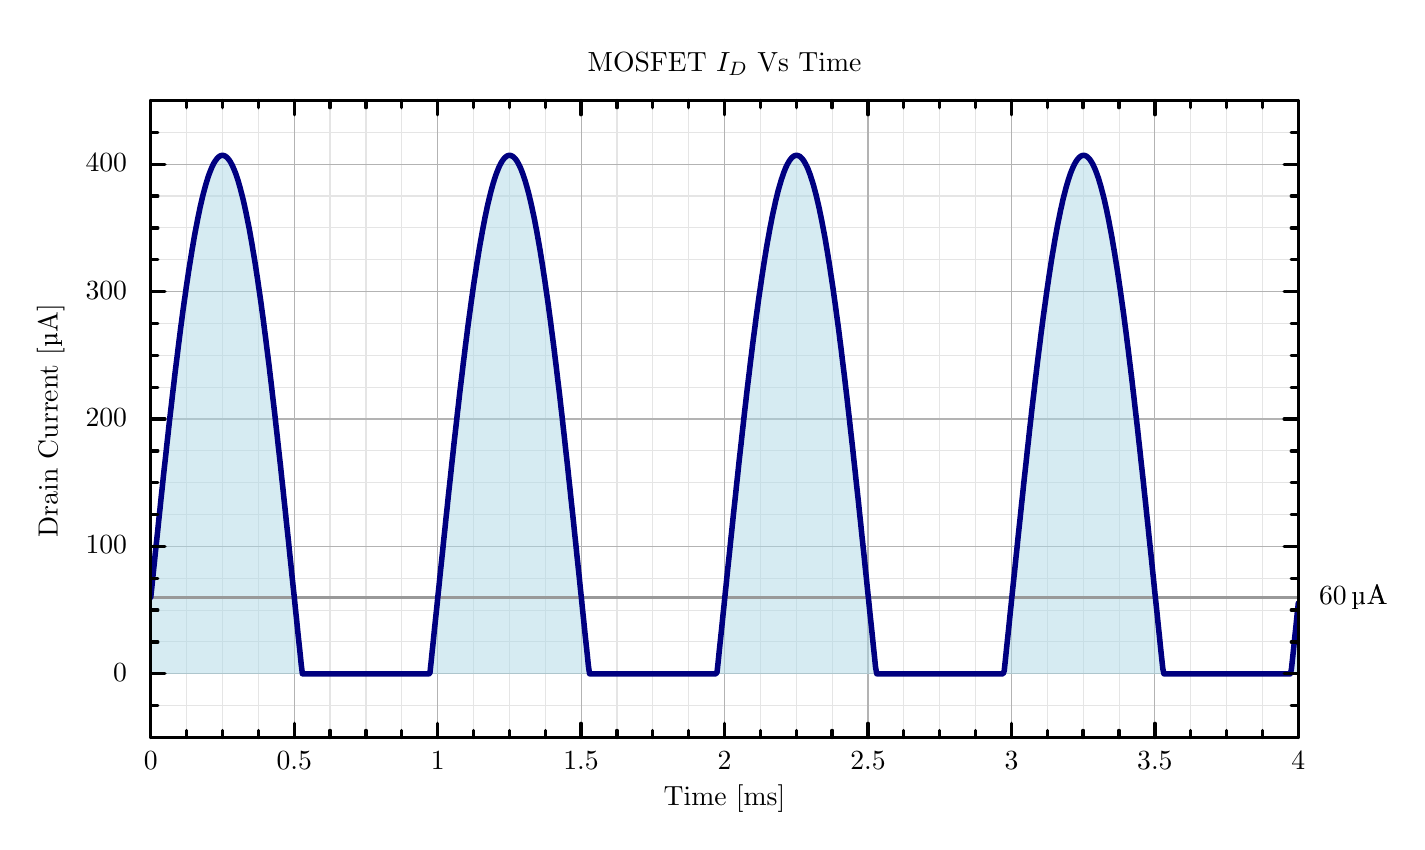
\begin{tikzpicture}[gnuplot]
%% generated with GNUPLOT 4.6p1 (Lua 5.1; terminal rev. 99, script rev. 100)
%% Sun 06 Oct 2013 15:18:02 EST
\path (0.000,0.000) rectangle (17.000,10.000);
\gpcolor{rgb color={0.898,0.898,0.898}}
\gpsetlinetype{gp lt border}
\gpsetlinewidth{1.00}
\draw[gp path] (1.504,0.985)--(16.079,0.985);
\draw[gp path] (1.504,1.390)--(16.079,1.390);
\gpcolor{color=gp lt color border}
\node[gp node right] at (1.320,1.794) { 0};
\gpcolor{rgb color={0.898,0.898,0.898}}
\draw[gp path] (1.504,2.199)--(16.079,2.199);
\draw[gp path] (1.504,2.603)--(16.079,2.603);
\draw[gp path] (1.504,3.008)--(16.079,3.008);
\gpcolor{color=gp lt color border}
\node[gp node right] at (1.320,3.412) { 100};
\gpcolor{rgb color={0.898,0.898,0.898}}
\draw[gp path] (1.504,3.817)--(16.079,3.817);
\draw[gp path] (1.504,4.221)--(16.079,4.221);
\draw[gp path] (1.504,4.626)--(16.079,4.626);
\gpcolor{color=gp lt color border}
\node[gp node right] at (1.320,5.030) { 200};
\gpcolor{rgb color={0.898,0.898,0.898}}
\draw[gp path] (1.504,5.435)--(16.079,5.435);
\draw[gp path] (1.504,5.839)--(16.079,5.839);
\draw[gp path] (1.504,6.244)--(16.079,6.244);
\gpcolor{color=gp lt color border}
\node[gp node right] at (1.320,6.648) { 300};
\gpcolor{rgb color={0.898,0.898,0.898}}
\draw[gp path] (1.504,7.053)--(16.079,7.053);
\draw[gp path] (1.504,7.457)--(16.079,7.457);
\draw[gp path] (1.504,7.862)--(16.079,7.862);
\gpcolor{color=gp lt color border}
\node[gp node right] at (1.320,8.266) { 400};
\gpcolor{rgb color={0.898,0.898,0.898}}
\draw[gp path] (1.504,8.671)--(16.079,8.671);
\draw[gp path] (1.504,9.075)--(16.079,9.075);
\gpcolor{color=gp lt color border}
\node[gp node center] at (1.504,0.677) { 0};
\gpcolor{rgb color={0.898,0.898,0.898}}
\draw[gp path] (1.959,0.985)--(1.959,9.075);
\draw[gp path] (2.415,0.985)--(2.415,9.075);
\draw[gp path] (2.870,0.985)--(2.870,9.075);
\gpcolor{color=gp lt color border}
\node[gp node center] at (3.326,0.677) { 0.5};
\gpcolor{rgb color={0.898,0.898,0.898}}
\draw[gp path] (3.781,0.985)--(3.781,9.075);
\draw[gp path] (4.237,0.985)--(4.237,9.075);
\draw[gp path] (4.692,0.985)--(4.692,9.075);
\gpcolor{color=gp lt color border}
\node[gp node center] at (5.148,0.677) { 1};
\gpcolor{rgb color={0.898,0.898,0.898}}
\draw[gp path] (5.603,0.985)--(5.603,9.075);
\draw[gp path] (6.059,0.985)--(6.059,9.075);
\draw[gp path] (6.514,0.985)--(6.514,9.075);
\gpcolor{color=gp lt color border}
\node[gp node center] at (6.970,0.677) { 1.5};
\gpcolor{rgb color={0.898,0.898,0.898}}
\draw[gp path] (7.425,0.985)--(7.425,9.075);
\draw[gp path] (7.881,0.985)--(7.881,9.075);
\draw[gp path] (8.336,0.985)--(8.336,9.075);
\gpcolor{color=gp lt color border}
\node[gp node center] at (8.792,0.677) { 2};
\gpcolor{rgb color={0.898,0.898,0.898}}
\draw[gp path] (9.247,0.985)--(9.247,9.075);
\draw[gp path] (9.702,0.985)--(9.702,9.075);
\draw[gp path] (10.158,0.985)--(10.158,9.075);
\gpcolor{color=gp lt color border}
\node[gp node center] at (10.613,0.677) { 2.5};
\gpcolor{rgb color={0.898,0.898,0.898}}
\draw[gp path] (11.069,0.985)--(11.069,9.075);
\draw[gp path] (11.524,0.985)--(11.524,9.075);
\draw[gp path] (11.980,0.985)--(11.980,9.075);
\gpcolor{color=gp lt color border}
\node[gp node center] at (12.435,0.677) { 3};
\gpcolor{rgb color={0.898,0.898,0.898}}
\draw[gp path] (12.891,0.985)--(12.891,9.075);
\draw[gp path] (13.346,0.985)--(13.346,9.075);
\draw[gp path] (13.802,0.985)--(13.802,9.075);
\gpcolor{color=gp lt color border}
\node[gp node center] at (14.257,0.677) { 3.5};
\gpcolor{rgb color={0.898,0.898,0.898}}
\draw[gp path] (14.713,0.985)--(14.713,9.075);
\draw[gp path] (15.168,0.985)--(15.168,9.075);
\draw[gp path] (15.624,0.985)--(15.624,9.075);
\gpcolor{color=gp lt color border}
\node[gp node center] at (16.079,0.677) { 4};
\node[gp node center,rotate=-270] at (0.246,5.030) {Drain Current [\si{\micro\ampere}]};
\node[gp node center] at (8.791,0.215) {Time [\si{\milli\second}]};
\node[gp node center] at (8.791,9.537) {MOSFET $I_D$ Vs Time};
\node[gp node left] at (16.225,2.765) {\SI{60}{\micro\ampere}};
%% coordinates of the plot area
\gpdefrectangularnode{gp plot 1}{\pgfpoint{1.504cm}{0.985cm}}{\pgfpoint{16.079cm}{9.075cm}}
\gpcolor{rgb color={0.702,0.702,0.702}}
\draw[gp path] (1.504,1.794)--(16.078,1.794);
\gpcolor{color=gp lt color border}
\gpcolor{rgb color={0.702,0.702,0.702}}
\draw[gp path] (1.504,3.412)--(16.078,3.412);
\gpcolor{color=gp lt color border}
\gpcolor{rgb color={0.702,0.702,0.702}}
\draw[gp path] (1.504,5.030)--(16.078,5.030);
\gpcolor{color=gp lt color border}
\gpcolor{rgb color={0.702,0.702,0.702}}
\draw[gp path] (1.504,6.647)--(16.078,6.647);
\gpcolor{color=gp lt color border}
\gpcolor{rgb color={0.702,0.702,0.702}}
\draw[gp path] (1.504,8.265)--(16.078,8.265);
\gpcolor{color=gp lt color border}
\gpcolor{rgb color={0.702,0.702,0.702}}
\draw[gp path] (1.504,0.985)--(1.504,9.074);
\gpcolor{color=gp lt color border}
\gpcolor{rgb color={0.702,0.702,0.702}}
\draw[gp path] (3.326,0.985)--(3.326,9.074);
\gpcolor{color=gp lt color border}
\gpcolor{rgb color={0.702,0.702,0.702}}
\draw[gp path] (5.148,0.985)--(5.148,9.074);
\gpcolor{color=gp lt color border}
\gpcolor{rgb color={0.702,0.702,0.702}}
\draw[gp path] (6.969,0.985)--(6.969,9.074);
\gpcolor{color=gp lt color border}
\gpcolor{rgb color={0.702,0.702,0.702}}
\draw[gp path] (8.791,0.985)--(8.791,9.074);
\gpcolor{color=gp lt color border}
\gpcolor{rgb color={0.702,0.702,0.702}}
\draw[gp path] (10.613,0.985)--(10.613,9.074);
\gpcolor{color=gp lt color border}
\gpcolor{rgb color={0.702,0.702,0.702}}
\draw[gp path] (12.435,0.985)--(12.435,9.074);
\gpcolor{color=gp lt color border}
\gpcolor{rgb color={0.702,0.702,0.702}}
\draw[gp path] (14.256,0.985)--(14.256,9.074);
\gpcolor{color=gp lt color border}
\gpcolor{rgb color={0.702,0.702,0.702}}
\draw[gp path] (16.078,0.985)--(16.078,9.074);
\gpcolor{color=gp lt color border}
%% coordinates of the plot area
\gpdefrectangularnode{gp plot 2}{\pgfpoint{1.504cm}{0.985cm}}{\pgfpoint{16.078cm}{9.074cm}}
\gpfill{rgb color={0.678,0.847,0.902},opacity=0.50} (1.504,2.765)--(1.504,2.765)--(1.519,2.906)--(1.533,3.047)%
    --(1.548,3.188)--(1.562,3.328)--(1.577,3.469)--(1.592,3.608)--(1.606,3.748)%
    --(1.621,3.886)--(1.635,4.024)--(1.650,4.161)--(1.664,4.298)--(1.679,4.433)%
    --(1.694,4.567)--(1.708,4.700)--(1.723,4.832)--(1.737,4.963)--(1.752,5.092)%
    --(1.767,5.220)--(1.781,5.346)--(1.796,5.470)--(1.810,5.593)--(1.825,5.714)%
    --(1.840,5.833)--(1.854,5.950)--(1.869,6.066)--(1.883,6.179)--(1.898,6.290)%
    --(1.912,6.398)--(1.927,6.505)--(1.942,6.609)--(1.956,6.711)--(1.971,6.810)%
    --(1.985,6.906)--(2.000,7.000)--(2.015,7.092)--(2.029,7.180)--(2.044,7.266)%
    --(2.058,7.349)--(2.073,7.429)--(2.088,7.506)--(2.102,7.580)--(2.117,7.651)%
    --(2.131,7.719)--(2.146,7.784)--(2.160,7.845)--(2.175,7.904)--(2.190,7.959)%
    --(2.204,8.011)--(2.219,8.059)--(2.233,8.105)--(2.248,8.147)--(2.263,8.185)%
    --(2.277,8.220)--(2.292,8.252)--(2.306,8.280)--(2.321,8.304)--(2.336,8.325)%
    --(2.350,8.343)--(2.365,8.357)--(2.379,8.368)--(2.394,8.375)--(2.408,8.378)%
    --(2.423,8.378)--(2.438,8.374)--(2.452,8.367)--(2.467,8.356)--(2.481,8.342)%
    --(2.496,8.324)--(2.511,8.303)--(2.525,8.278)--(2.540,8.250)--(2.554,8.218)%
    --(2.569,8.183)--(2.584,8.144)--(2.598,8.102)--(2.613,8.057)--(2.627,8.008)%
    --(2.642,7.956)--(2.656,7.900)--(2.671,7.842)--(2.686,7.780)--(2.700,7.715)%
    --(2.715,7.647)--(2.729,7.576)--(2.744,7.501)--(2.759,7.424)--(2.773,7.344)%
    --(2.788,7.261)--(2.802,7.175)--(2.817,7.086)--(2.832,6.995)--(2.846,6.900)%
    --(2.861,6.804)--(2.875,6.704)--(2.890,6.603)--(2.905,6.498)--(2.919,6.392)%
    --(2.934,6.283)--(2.948,6.172)--(2.963,6.059)--(2.977,5.943)--(2.992,5.826)%
    --(3.007,5.707)--(3.021,5.586)--(3.036,5.463)--(3.050,5.338)--(3.065,5.212)%
    --(3.080,5.084)--(3.094,4.955)--(3.109,4.824)--(3.123,4.692)--(3.138,4.559)%
    --(3.153,4.425)--(3.167,4.289)--(3.182,4.153)--(3.196,4.016)--(3.211,3.878)%
    --(3.225,3.739)--(3.240,3.600)--(3.255,3.460)--(3.269,3.320)--(3.284,3.179)%
    --(3.298,3.038)--(3.313,2.897)--(3.328,2.756)--(3.342,2.615)--(3.357,2.474)%
    --(3.371,2.333)--(3.386,2.192)--(3.401,2.052)--(3.415,1.912)--(3.430,1.794)%
    --(3.444,1.794)--(3.459,1.794)--(3.473,1.794)--(3.488,1.794)--(3.503,1.794)%
    --(3.517,1.794)--(3.532,1.794)--(3.546,1.794)--(3.561,1.794)--(3.576,1.794)%
    --(3.590,1.794)--(3.605,1.794)--(3.619,1.794)--(3.634,1.794)--(3.649,1.794)%
    --(3.663,1.794)--(3.678,1.794)--(3.692,1.794)--(3.707,1.794)--(3.721,1.794)%
    --(3.736,1.794)--(3.751,1.794)--(3.765,1.794)--(3.780,1.794)--(3.794,1.794)%
    --(3.809,1.794)--(3.824,1.794)--(3.838,1.794)--(3.853,1.794)--(3.867,1.794)%
    --(3.882,1.794)--(3.897,1.794)--(3.911,1.794)--(3.926,1.794)--(3.940,1.794)%
    --(3.955,1.794)--(3.969,1.794)--(3.984,1.794)--(3.999,1.794)--(4.013,1.794)%
    --(4.028,1.794)--(4.042,1.794)--(4.057,1.794)--(4.072,1.794)--(4.086,1.794)%
    --(4.101,1.794)--(4.115,1.794)--(4.130,1.794)--(4.145,1.794)--(4.159,1.794)%
    --(4.174,1.794)--(4.188,1.794)--(4.203,1.794)--(4.217,1.794)--(4.232,1.794)%
    --(4.247,1.794)--(4.261,1.794)--(4.276,1.794)--(4.290,1.794)--(4.305,1.794)%
    --(4.320,1.794)--(4.334,1.794)--(4.349,1.794)--(4.363,1.794)--(4.378,1.794)%
    --(4.393,1.794)--(4.407,1.794)--(4.422,1.794)--(4.436,1.794)--(4.451,1.794)%
    --(4.465,1.794)--(4.480,1.794)--(4.495,1.794)--(4.509,1.794)--(4.524,1.794)%
    --(4.538,1.794)--(4.553,1.794)--(4.568,1.794)--(4.582,1.794)--(4.597,1.794)%
    --(4.611,1.794)--(4.626,1.794)--(4.641,1.794)--(4.655,1.794)--(4.670,1.794)%
    --(4.684,1.794)--(4.699,1.794)--(4.713,1.794)--(4.728,1.794)--(4.743,1.794)%
    --(4.757,1.794)--(4.772,1.794)--(4.786,1.794)--(4.801,1.794)--(4.816,1.794)%
    --(4.830,1.794)--(4.845,1.794)--(4.859,1.794)--(4.874,1.794)--(4.889,1.794)%
    --(4.903,1.794)--(4.918,1.794)--(4.932,1.794)--(4.947,1.794)--(4.961,1.794)%
    --(4.976,1.794)--(4.991,1.794)--(5.005,1.794)--(5.020,1.794)--(5.034,1.794)%
    --(5.049,1.799)--(5.064,1.938)--(5.078,2.078)--(5.093,2.218)--(5.107,2.359)%
    --(5.122,2.500)--(5.137,2.641)--(5.151,2.782)--(5.166,2.923)--(5.180,3.064)%
    --(5.195,3.205)--(5.210,3.346)--(5.224,3.486)--(5.239,3.626)--(5.253,3.765)%
    --(5.268,3.903)--(5.282,4.041)--(5.297,4.178)--(5.312,4.314)--(5.326,4.450)%
    --(5.341,4.584)--(5.355,4.717)--(5.370,4.848)--(5.385,4.979)--(5.399,5.108)%
    --(5.414,5.235)--(5.428,5.361)--(5.443,5.485)--(5.458,5.608)--(5.472,5.729)%
    --(5.487,5.848)--(5.501,5.965)--(5.516,6.080)--(5.530,6.193)--(5.545,6.303)%
    --(5.560,6.412)--(5.574,6.518)--(5.589,6.622)--(5.603,6.723)--(5.618,6.822)%
    --(5.633,6.918)--(5.647,7.012)--(5.662,7.103)--(5.676,7.191)--(5.691,7.276)%
    --(5.706,7.359)--(5.720,7.439)--(5.735,7.515)--(5.749,7.589)--(5.764,7.660)%
    --(5.778,7.727)--(5.793,7.792)--(5.808,7.853)--(5.822,7.911)--(5.837,7.966)%
    --(5.851,8.017)--(5.866,8.065)--(5.881,8.110)--(5.895,8.151)--(5.910,8.189)%
    --(5.924,8.224)--(5.939,8.255)--(5.954,8.283)--(5.968,8.307)--(5.983,8.328)%
    --(5.997,8.345)--(6.012,8.358)--(6.026,8.369)--(6.041,8.375)--(6.056,8.378)%
    --(6.070,8.378)--(6.085,8.373)--(6.099,8.366)--(6.114,8.355)--(6.129,8.340)%
    --(6.143,8.322)--(6.158,8.300)--(6.172,8.275)--(6.187,8.246)--(6.202,8.214)%
    --(6.216,8.178)--(6.231,8.139)--(6.245,8.097)--(6.260,8.051)--(6.274,8.002)%
    --(6.289,7.949)--(6.304,7.893)--(6.318,7.834)--(6.333,7.772)--(6.347,7.707)%
    --(6.362,7.638)--(6.377,7.567)--(6.391,7.492)--(6.406,7.414)--(6.420,7.334)%
    --(6.435,7.250)--(6.450,7.164)--(6.464,7.075)--(6.479,6.983)--(6.493,6.889)%
    --(6.508,6.792)--(6.522,6.692)--(6.537,6.590)--(6.552,6.485)--(6.566,6.379)%
    --(6.581,6.269)--(6.595,6.158)--(6.610,6.045)--(6.625,5.929)--(6.639,5.811)%
    --(6.654,5.692)--(6.668,5.570)--(6.683,5.447)--(6.698,5.323)--(6.712,5.196)%
    --(6.727,5.068)--(6.741,4.939)--(6.756,4.808)--(6.770,4.676)--(6.785,4.542)%
    --(6.800,4.408)--(6.814,4.272)--(6.829,4.136)--(6.843,3.999)--(6.858,3.861)%
    --(6.873,3.722)--(6.887,3.582)--(6.902,3.443)--(6.916,3.302)--(6.931,3.162)%
    --(6.946,3.021)--(6.960,2.880)--(6.975,2.738)--(6.989,2.597)--(7.004,2.456)%
    --(7.018,2.315)--(7.033,2.175)--(7.048,2.035)--(7.062,1.895)--(7.077,1.794)%
    --(7.091,1.794)--(7.106,1.794)--(7.121,1.794)--(7.135,1.794)--(7.150,1.794)%
    --(7.164,1.794)--(7.179,1.794)--(7.194,1.794)--(7.208,1.794)--(7.223,1.794)%
    --(7.237,1.794)--(7.252,1.794)--(7.266,1.794)--(7.281,1.794)--(7.296,1.794)%
    --(7.310,1.794)--(7.325,1.794)--(7.339,1.794)--(7.354,1.794)--(7.369,1.794)%
    --(7.383,1.794)--(7.398,1.794)--(7.412,1.794)--(7.427,1.794)--(7.442,1.794)%
    --(7.456,1.794)--(7.471,1.794)--(7.485,1.794)--(7.500,1.794)--(7.514,1.794)%
    --(7.529,1.794)--(7.544,1.794)--(7.558,1.794)--(7.573,1.794)--(7.587,1.794)%
    --(7.602,1.794)--(7.617,1.794)--(7.631,1.794)--(7.646,1.794)--(7.660,1.794)%
    --(7.675,1.794)--(7.690,1.794)--(7.704,1.794)--(7.719,1.794)--(7.733,1.794)%
    --(7.748,1.794)--(7.763,1.794)--(7.777,1.794)--(7.792,1.794)--(7.806,1.794)%
    --(7.821,1.794)--(7.835,1.794)--(7.850,1.794)--(7.865,1.794)--(7.879,1.794)%
    --(7.894,1.794)--(7.908,1.794)--(7.923,1.794)--(7.938,1.794)--(7.952,1.794)%
    --(7.967,1.794)--(7.981,1.794)--(7.996,1.794)--(8.011,1.794)--(8.025,1.794)%
    --(8.040,1.794)--(8.054,1.794)--(8.069,1.794)--(8.083,1.794)--(8.098,1.794)%
    --(8.113,1.794)--(8.127,1.794)--(8.142,1.794)--(8.156,1.794)--(8.171,1.794)%
    --(8.186,1.794)--(8.200,1.794)--(8.215,1.794)--(8.229,1.794)--(8.244,1.794)%
    --(8.259,1.794)--(8.273,1.794)--(8.288,1.794)--(8.302,1.794)--(8.317,1.794)%
    --(8.331,1.794)--(8.346,1.794)--(8.361,1.794)--(8.375,1.794)--(8.390,1.794)%
    --(8.404,1.794)--(8.419,1.794)--(8.434,1.794)--(8.448,1.794)--(8.463,1.794)%
    --(8.477,1.794)--(8.492,1.794)--(8.507,1.794)--(8.521,1.794)--(8.536,1.794)%
    --(8.550,1.794)--(8.565,1.794)--(8.579,1.794)--(8.594,1.794)--(8.609,1.794)%
    --(8.623,1.794)--(8.638,1.794)--(8.652,1.794)--(8.667,1.794)--(8.682,1.794)%
    --(8.696,1.816)--(8.711,1.955)--(8.725,2.095)--(8.740,2.236)--(8.755,2.376)%
    --(8.769,2.517)--(8.784,2.658)--(8.798,2.799)--(8.813,2.941)--(8.827,3.082)%
    --(8.842,3.222)--(8.857,3.363)--(8.871,3.503)--(8.886,3.643)--(8.900,3.782)%
    --(8.915,3.920)--(8.930,4.058)--(8.944,4.195)--(8.959,4.331)--(8.973,4.466)%
    --(8.988,4.600)--(9.003,4.733)--(9.017,4.864)--(9.032,4.995)--(9.046,5.124)%
    --(9.061,5.251)--(9.075,5.377)--(9.090,5.501)--(9.105,5.623)--(9.119,5.744)%
    --(9.134,5.862)--(9.148,5.979)--(9.163,6.094)--(9.178,6.206)--(9.192,6.317)%
    --(9.207,6.425)--(9.221,6.531)--(9.236,6.634)--(9.251,6.735)--(9.265,6.834)%
    --(9.280,6.930)--(9.294,7.023)--(9.309,7.114)--(9.323,7.202)--(9.338,7.287)%
    --(9.353,7.369)--(9.367,7.448)--(9.382,7.524)--(9.396,7.598)--(9.411,7.668)%
    --(9.426,7.735)--(9.440,7.799)--(9.455,7.860)--(9.469,7.918)--(9.484,7.972)%
    --(9.499,8.023)--(9.513,8.071)--(9.528,8.115)--(9.542,8.156)--(9.557,8.194)%
    --(9.571,8.228)--(9.586,8.259)--(9.601,8.286)--(9.615,8.310)--(9.630,8.330)%
    --(9.644,8.347)--(9.659,8.360)--(9.674,8.370)--(9.688,8.376)--(9.703,8.378)%
    --(9.717,8.377)--(9.732,8.373)--(9.747,8.365)--(9.761,8.353)--(9.776,8.338)%
    --(9.790,8.319)--(9.805,8.297)--(9.819,8.271)--(9.834,8.242)--(9.849,8.210)%
    --(9.863,8.173)--(9.878,8.134)--(9.892,8.091)--(9.907,8.045)--(9.922,7.995)%
    --(9.936,7.942)--(9.951,7.886)--(9.965,7.827)--(9.980,7.764)--(9.995,7.698)%
    --(10.009,7.629)--(10.024,7.557)--(10.038,7.482)--(10.053,7.405)--(10.068,7.324)%
    --(10.082,7.240)--(10.097,7.153)--(10.111,7.064)--(10.126,6.972)--(10.140,6.877)%
    --(10.155,6.779)--(10.170,6.680)--(10.184,6.577)--(10.199,6.472)--(10.213,6.365)%
    --(10.228,6.256)--(10.243,6.144)--(10.257,6.030)--(10.272,5.915)--(10.286,5.797)%
    --(10.301,5.677)--(10.316,5.555)--(10.330,5.432)--(10.345,5.307)--(10.359,5.180)%
    --(10.374,5.052)--(10.388,4.923)--(10.403,4.792)--(10.418,4.659)--(10.432,4.526)%
    --(10.447,4.391)--(10.461,4.256)--(10.476,4.119)--(10.491,3.982)--(10.505,3.844)%
    --(10.520,3.705)--(10.534,3.565)--(10.549,3.425)--(10.564,3.285)--(10.578,3.144)%
    --(10.593,3.003)--(10.607,2.862)--(10.622,2.721)--(10.636,2.580)--(10.651,2.439)%
    --(10.666,2.298)--(10.680,2.158)--(10.695,2.017)--(10.709,1.878)--(10.724,1.794)%
    --(10.739,1.794)--(10.753,1.794)--(10.768,1.794)--(10.782,1.794)--(10.797,1.794)%
    --(10.812,1.794)--(10.826,1.794)--(10.841,1.794)--(10.855,1.794)--(10.870,1.794)%
    --(10.884,1.794)--(10.899,1.794)--(10.914,1.794)--(10.928,1.794)--(10.943,1.794)%
    --(10.957,1.794)--(10.972,1.794)--(10.987,1.794)--(11.001,1.794)--(11.016,1.794)%
    --(11.030,1.794)--(11.045,1.794)--(11.060,1.794)--(11.074,1.794)--(11.089,1.794)%
    --(11.103,1.794)--(11.118,1.794)--(11.132,1.794)--(11.147,1.794)--(11.162,1.794)%
    --(11.176,1.794)--(11.191,1.794)--(11.205,1.794)--(11.220,1.794)--(11.235,1.794)%
    --(11.249,1.794)--(11.264,1.794)--(11.278,1.794)--(11.293,1.794)--(11.308,1.794)%
    --(11.322,1.794)--(11.337,1.794)--(11.351,1.794)--(11.366,1.794)--(11.380,1.794)%
    --(11.395,1.794)--(11.410,1.794)--(11.424,1.794)--(11.439,1.794)--(11.453,1.794)%
    --(11.468,1.794)--(11.483,1.794)--(11.497,1.794)--(11.512,1.794)--(11.526,1.794)%
    --(11.541,1.794)--(11.556,1.794)--(11.570,1.794)--(11.585,1.794)--(11.599,1.794)%
    --(11.614,1.794)--(11.628,1.794)--(11.643,1.794)--(11.658,1.794)--(11.672,1.794)%
    --(11.687,1.794)--(11.701,1.794)--(11.716,1.794)--(11.731,1.794)--(11.745,1.794)%
    --(11.760,1.794)--(11.774,1.794)--(11.789,1.794)--(11.804,1.794)--(11.818,1.794)%
    --(11.833,1.794)--(11.847,1.794)--(11.862,1.794)--(11.876,1.794)--(11.891,1.794)%
    --(11.906,1.794)--(11.920,1.794)--(11.935,1.794)--(11.949,1.794)--(11.964,1.794)%
    --(11.979,1.794)--(11.993,1.794)--(12.008,1.794)--(12.022,1.794)--(12.037,1.794)%
    --(12.052,1.794)--(12.066,1.794)--(12.081,1.794)--(12.095,1.794)--(12.110,1.794)%
    --(12.124,1.794)--(12.139,1.794)--(12.154,1.794)--(12.168,1.794)--(12.183,1.794)%
    --(12.197,1.794)--(12.212,1.794)--(12.227,1.794)--(12.241,1.794)--(12.256,1.794)%
    --(12.270,1.794)--(12.285,1.794)--(12.300,1.794)--(12.314,1.794)--(12.329,1.794)%
    --(12.343,1.833)--(12.358,1.973)--(12.372,2.112)--(12.387,2.253)--(12.402,2.394)%
    --(12.416,2.535)--(12.431,2.676)--(12.445,2.817)--(12.460,2.958)--(12.475,3.099)%
    --(12.489,3.240)--(12.504,3.380)--(12.518,3.520)--(12.533,3.660)--(12.548,3.799)%
    --(12.562,3.937)--(12.577,4.075)--(12.591,4.212)--(12.606,4.348)--(12.621,4.483)%
    --(12.635,4.617)--(12.650,4.749)--(12.664,4.881)--(12.679,5.011)--(12.693,5.139)%
    --(12.708,5.266)--(12.723,5.392)--(12.737,5.516)--(12.752,5.638)--(12.766,5.758)%
    --(12.781,5.877)--(12.796,5.993)--(12.810,6.108)--(12.825,6.220)--(12.839,6.330)%
    --(12.854,6.438)--(12.869,6.544)--(12.883,6.647)--(12.898,6.748)--(12.912,6.846)%
    --(12.927,6.941)--(12.941,7.034)--(12.956,7.125)--(12.971,7.212)--(12.985,7.297)%
    --(13.000,7.379)--(13.014,7.458)--(13.029,7.534)--(13.044,7.607)--(13.058,7.677)%
    --(13.073,7.743)--(13.087,7.807)--(13.102,7.867)--(13.117,7.925)--(13.131,7.979)%
    --(13.146,8.029)--(13.160,8.077)--(13.175,8.121)--(13.189,8.161)--(13.204,8.198)%
    --(13.219,8.232)--(13.233,8.262)--(13.248,8.289)--(13.262,8.312)--(13.277,8.332)%
    --(13.292,8.349)--(13.306,8.361)--(13.321,8.371)--(13.335,8.376)--(13.350,8.378)%
    --(13.365,8.377)--(13.379,8.372)--(13.394,8.363)--(13.408,8.351)--(13.423,8.336)%
    --(13.437,8.317)--(13.452,8.294)--(13.467,8.268)--(13.481,8.238)--(13.496,8.205)%
    --(13.510,8.169)--(13.525,8.129)--(13.540,8.086)--(13.554,8.039)--(13.569,7.989)%
    --(13.583,7.936)--(13.598,7.879)--(13.613,7.819)--(13.627,7.756)--(13.642,7.690)%
    --(13.656,7.621)--(13.671,7.548)--(13.685,7.473)--(13.700,7.395)--(13.715,7.313)%
    --(13.729,7.229)--(13.744,7.142)--(13.758,7.053)--(13.773,6.960)--(13.788,6.865)%
    --(13.802,6.767)--(13.817,6.667)--(13.831,6.564)--(13.846,6.459)--(13.861,6.352)%
    --(13.875,6.242)--(13.890,6.130)--(13.904,6.016)--(13.919,5.900)--(13.933,5.782)%
    --(13.948,5.662)--(13.963,5.540)--(13.977,5.417)--(13.992,5.291)--(14.006,5.165)%
    --(14.021,5.036)--(14.036,4.906)--(14.050,4.775)--(14.065,4.643)--(14.079,4.509)%
    --(14.094,4.375)--(14.109,4.239)--(14.123,4.102)--(14.138,3.965)--(14.152,3.826)%
    --(14.167,3.688)--(14.181,3.548)--(14.196,3.408)--(14.211,3.268)--(14.225,3.127)%
    --(14.240,2.986)--(14.254,2.845)--(14.269,2.704)--(14.284,2.563)--(14.298,2.422)%
    --(14.313,2.281)--(14.327,2.140)--(14.342,2.000)--(14.357,1.861)--(14.371,1.794)%
    --(14.386,1.794)--(14.400,1.794)--(14.415,1.794)--(14.429,1.794)--(14.444,1.794)%
    --(14.459,1.794)--(14.473,1.794)--(14.488,1.794)--(14.502,1.794)--(14.517,1.794)%
    --(14.532,1.794)--(14.546,1.794)--(14.561,1.794)--(14.575,1.794)--(14.590,1.794)%
    --(14.605,1.794)--(14.619,1.794)--(14.634,1.794)--(14.648,1.794)--(14.663,1.794)%
    --(14.677,1.794)--(14.692,1.794)--(14.707,1.794)--(14.721,1.794)--(14.736,1.794)%
    --(14.750,1.794)--(14.765,1.794)--(14.780,1.794)--(14.794,1.794)--(14.809,1.794)%
    --(14.823,1.794)--(14.838,1.794)--(14.853,1.794)--(14.867,1.794)--(14.882,1.794)%
    --(14.896,1.794)--(14.911,1.794)--(14.926,1.794)--(14.940,1.794)--(14.955,1.794)%
    --(14.969,1.794)--(14.984,1.794)--(14.998,1.794)--(15.013,1.794)--(15.028,1.794)%
    --(15.042,1.794)--(15.057,1.794)--(15.071,1.794)--(15.086,1.794)--(15.101,1.794)%
    --(15.115,1.794)--(15.130,1.794)--(15.144,1.794)--(15.159,1.794)--(15.174,1.794)%
    --(15.188,1.794)--(15.203,1.794)--(15.217,1.794)--(15.232,1.794)--(15.246,1.794)%
    --(15.261,1.794)--(15.276,1.794)--(15.290,1.794)--(15.305,1.794)--(15.319,1.794)%
    --(15.334,1.794)--(15.349,1.794)--(15.363,1.794)--(15.378,1.794)--(15.392,1.794)%
    --(15.407,1.794)--(15.422,1.794)--(15.436,1.794)--(15.451,1.794)--(15.465,1.794)%
    --(15.480,1.794)--(15.494,1.794)--(15.509,1.794)--(15.524,1.794)--(15.538,1.794)%
    --(15.553,1.794)--(15.567,1.794)--(15.582,1.794)--(15.597,1.794)--(15.611,1.794)%
    --(15.626,1.794)--(15.640,1.794)--(15.655,1.794)--(15.670,1.794)--(15.684,1.794)%
    --(15.699,1.794)--(15.713,1.794)--(15.728,1.794)--(15.742,1.794)--(15.757,1.794)%
    --(15.772,1.794)--(15.786,1.794)--(15.801,1.794)--(15.815,1.794)--(15.830,1.794)%
    --(15.845,1.794)--(15.859,1.794)--(15.874,1.794)--(15.888,1.794)--(15.903,1.794)%
    --(15.918,1.794)--(15.932,1.794)--(15.947,1.794)--(15.961,1.794)--(15.976,1.794)%
    --(15.990,1.850)--(16.005,1.990)--(16.020,2.130)--(16.034,2.270)--(16.049,2.411)%
    --(16.063,2.552)--(16.078,2.693)--(16.078,1.794)--(1.504,1.794)--cycle;
\gpcolor{rgb color={0.600,0.600,0.600}}
\gpsetlinetype{gp lt plot 1}
\gpsetlinewidth{3.00}
\draw[gp path] (1.504,2.765)--(1.519,2.765)--(1.533,2.765)--(1.548,2.765)--(1.562,2.765)%
  --(1.577,2.765)--(1.592,2.765)--(1.606,2.765)--(1.621,2.765)--(1.635,2.765)--(1.650,2.765)%
  --(1.664,2.765)--(1.679,2.765)--(1.694,2.765)--(1.708,2.765)--(1.723,2.765)--(1.737,2.765)%
  --(1.752,2.765)--(1.767,2.765)--(1.781,2.765)--(1.796,2.765)--(1.810,2.765)--(1.825,2.765)%
  --(1.840,2.765)--(1.854,2.765)--(1.869,2.765)--(1.883,2.765)--(1.898,2.765)--(1.912,2.765)%
  --(1.927,2.765)--(1.942,2.765)--(1.956,2.765)--(1.971,2.765)--(1.985,2.765)--(2.000,2.765)%
  --(2.015,2.765)--(2.029,2.765)--(2.044,2.765)--(2.058,2.765)--(2.073,2.765)--(2.088,2.765)%
  --(2.102,2.765)--(2.117,2.765)--(2.131,2.765)--(2.146,2.765)--(2.160,2.765)--(2.175,2.765)%
  --(2.190,2.765)--(2.204,2.765)--(2.219,2.765)--(2.233,2.765)--(2.248,2.765)--(2.263,2.765)%
  --(2.277,2.765)--(2.292,2.765)--(2.306,2.765)--(2.321,2.765)--(2.336,2.765)--(2.350,2.765)%
  --(2.365,2.765)--(2.379,2.765)--(2.394,2.765)--(2.408,2.765)--(2.423,2.765)--(2.438,2.765)%
  --(2.452,2.765)--(2.467,2.765)--(2.481,2.765)--(2.496,2.765)--(2.511,2.765)--(2.525,2.765)%
  --(2.540,2.765)--(2.554,2.765)--(2.569,2.765)--(2.584,2.765)--(2.598,2.765)--(2.613,2.765)%
  --(2.627,2.765)--(2.642,2.765)--(2.656,2.765)--(2.671,2.765)--(2.686,2.765)--(2.700,2.765)%
  --(2.715,2.765)--(2.729,2.765)--(2.744,2.765)--(2.759,2.765)--(2.773,2.765)--(2.788,2.765)%
  --(2.802,2.765)--(2.817,2.765)--(2.832,2.765)--(2.846,2.765)--(2.861,2.765)--(2.875,2.765)%
  --(2.890,2.765)--(2.905,2.765)--(2.919,2.765)--(2.934,2.765)--(2.948,2.765)--(2.963,2.765)%
  --(2.977,2.765)--(2.992,2.765)--(3.007,2.765)--(3.021,2.765)--(3.036,2.765)--(3.050,2.765)%
  --(3.065,2.765)--(3.080,2.765)--(3.094,2.765)--(3.109,2.765)--(3.123,2.765)--(3.138,2.765)%
  --(3.153,2.765)--(3.167,2.765)--(3.182,2.765)--(3.196,2.765)--(3.211,2.765)--(3.225,2.765)%
  --(3.240,2.765)--(3.255,2.765)--(3.269,2.765)--(3.284,2.765)--(3.298,2.765)--(3.313,2.765)%
  --(3.328,2.765)--(3.342,2.765)--(3.357,2.765)--(3.371,2.765)--(3.386,2.765)--(3.401,2.765)%
  --(3.415,2.765)--(3.430,2.765)--(3.444,2.765)--(3.459,2.765)--(3.473,2.765)--(3.488,2.765)%
  --(3.503,2.765)--(3.517,2.765)--(3.532,2.765)--(3.546,2.765)--(3.561,2.765)--(3.576,2.765)%
  --(3.590,2.765)--(3.605,2.765)--(3.619,2.765)--(3.634,2.765)--(3.649,2.765)--(3.663,2.765)%
  --(3.678,2.765)--(3.692,2.765)--(3.707,2.765)--(3.721,2.765)--(3.736,2.765)--(3.751,2.765)%
  --(3.765,2.765)--(3.780,2.765)--(3.794,2.765)--(3.809,2.765)--(3.824,2.765)--(3.838,2.765)%
  --(3.853,2.765)--(3.867,2.765)--(3.882,2.765)--(3.897,2.765)--(3.911,2.765)--(3.926,2.765)%
  --(3.940,2.765)--(3.955,2.765)--(3.969,2.765)--(3.984,2.765)--(3.999,2.765)--(4.013,2.765)%
  --(4.028,2.765)--(4.042,2.765)--(4.057,2.765)--(4.072,2.765)--(4.086,2.765)--(4.101,2.765)%
  --(4.115,2.765)--(4.130,2.765)--(4.145,2.765)--(4.159,2.765)--(4.174,2.765)--(4.188,2.765)%
  --(4.203,2.765)--(4.217,2.765)--(4.232,2.765)--(4.247,2.765)--(4.261,2.765)--(4.276,2.765)%
  --(4.290,2.765)--(4.305,2.765)--(4.320,2.765)--(4.334,2.765)--(4.349,2.765)--(4.363,2.765)%
  --(4.378,2.765)--(4.393,2.765)--(4.407,2.765)--(4.422,2.765)--(4.436,2.765)--(4.451,2.765)%
  --(4.465,2.765)--(4.480,2.765)--(4.495,2.765)--(4.509,2.765)--(4.524,2.765)--(4.538,2.765)%
  --(4.553,2.765)--(4.568,2.765)--(4.582,2.765)--(4.597,2.765)--(4.611,2.765)--(4.626,2.765)%
  --(4.641,2.765)--(4.655,2.765)--(4.670,2.765)--(4.684,2.765)--(4.699,2.765)--(4.713,2.765)%
  --(4.728,2.765)--(4.743,2.765)--(4.757,2.765)--(4.772,2.765)--(4.786,2.765)--(4.801,2.765)%
  --(4.816,2.765)--(4.830,2.765)--(4.845,2.765)--(4.859,2.765)--(4.874,2.765)--(4.889,2.765)%
  --(4.903,2.765)--(4.918,2.765)--(4.932,2.765)--(4.947,2.765)--(4.961,2.765)--(4.976,2.765)%
  --(4.991,2.765)--(5.005,2.765)--(5.020,2.765)--(5.034,2.765)--(5.049,2.765)--(5.064,2.765)%
  --(5.078,2.765)--(5.093,2.765)--(5.107,2.765)--(5.122,2.765)--(5.137,2.765)--(5.151,2.765)%
  --(5.166,2.765)--(5.180,2.765)--(5.195,2.765)--(5.210,2.765)--(5.224,2.765)--(5.239,2.765)%
  --(5.253,2.765)--(5.268,2.765)--(5.282,2.765)--(5.297,2.765)--(5.312,2.765)--(5.326,2.765)%
  --(5.341,2.765)--(5.355,2.765)--(5.370,2.765)--(5.385,2.765)--(5.399,2.765)--(5.414,2.765)%
  --(5.428,2.765)--(5.443,2.765)--(5.458,2.765)--(5.472,2.765)--(5.487,2.765)--(5.501,2.765)%
  --(5.516,2.765)--(5.530,2.765)--(5.545,2.765)--(5.560,2.765)--(5.574,2.765)--(5.589,2.765)%
  --(5.603,2.765)--(5.618,2.765)--(5.633,2.765)--(5.647,2.765)--(5.662,2.765)--(5.676,2.765)%
  --(5.691,2.765)--(5.706,2.765)--(5.720,2.765)--(5.735,2.765)--(5.749,2.765)--(5.764,2.765)%
  --(5.778,2.765)--(5.793,2.765)--(5.808,2.765)--(5.822,2.765)--(5.837,2.765)--(5.851,2.765)%
  --(5.866,2.765)--(5.881,2.765)--(5.895,2.765)--(5.910,2.765)--(5.924,2.765)--(5.939,2.765)%
  --(5.954,2.765)--(5.968,2.765)--(5.983,2.765)--(5.997,2.765)--(6.012,2.765)--(6.026,2.765)%
  --(6.041,2.765)--(6.056,2.765)--(6.070,2.765)--(6.085,2.765)--(6.099,2.765)--(6.114,2.765)%
  --(6.129,2.765)--(6.143,2.765)--(6.158,2.765)--(6.172,2.765)--(6.187,2.765)--(6.202,2.765)%
  --(6.216,2.765)--(6.231,2.765)--(6.245,2.765)--(6.260,2.765)--(6.274,2.765)--(6.289,2.765)%
  --(6.304,2.765)--(6.318,2.765)--(6.333,2.765)--(6.347,2.765)--(6.362,2.765)--(6.377,2.765)%
  --(6.391,2.765)--(6.406,2.765)--(6.420,2.765)--(6.435,2.765)--(6.450,2.765)--(6.464,2.765)%
  --(6.479,2.765)--(6.493,2.765)--(6.508,2.765)--(6.522,2.765)--(6.537,2.765)--(6.552,2.765)%
  --(6.566,2.765)--(6.581,2.765)--(6.595,2.765)--(6.610,2.765)--(6.625,2.765)--(6.639,2.765)%
  --(6.654,2.765)--(6.668,2.765)--(6.683,2.765)--(6.698,2.765)--(6.712,2.765)--(6.727,2.765)%
  --(6.741,2.765)--(6.756,2.765)--(6.770,2.765)--(6.785,2.765)--(6.800,2.765)--(6.814,2.765)%
  --(6.829,2.765)--(6.843,2.765)--(6.858,2.765)--(6.873,2.765)--(6.887,2.765)--(6.902,2.765)%
  --(6.916,2.765)--(6.931,2.765)--(6.946,2.765)--(6.960,2.765)--(6.975,2.765)--(6.989,2.765)%
  --(7.004,2.765)--(7.018,2.765)--(7.033,2.765)--(7.048,2.765)--(7.062,2.765)--(7.077,2.765)%
  --(7.091,2.765)--(7.106,2.765)--(7.121,2.765)--(7.135,2.765)--(7.150,2.765)--(7.164,2.765)%
  --(7.179,2.765)--(7.194,2.765)--(7.208,2.765)--(7.223,2.765)--(7.237,2.765)--(7.252,2.765)%
  --(7.266,2.765)--(7.281,2.765)--(7.296,2.765)--(7.310,2.765)--(7.325,2.765)--(7.339,2.765)%
  --(7.354,2.765)--(7.369,2.765)--(7.383,2.765)--(7.398,2.765)--(7.412,2.765)--(7.427,2.765)%
  --(7.442,2.765)--(7.456,2.765)--(7.471,2.765)--(7.485,2.765)--(7.500,2.765)--(7.514,2.765)%
  --(7.529,2.765)--(7.544,2.765)--(7.558,2.765)--(7.573,2.765)--(7.587,2.765)--(7.602,2.765)%
  --(7.617,2.765)--(7.631,2.765)--(7.646,2.765)--(7.660,2.765)--(7.675,2.765)--(7.690,2.765)%
  --(7.704,2.765)--(7.719,2.765)--(7.733,2.765)--(7.748,2.765)--(7.763,2.765)--(7.777,2.765)%
  --(7.792,2.765)--(7.806,2.765)--(7.821,2.765)--(7.835,2.765)--(7.850,2.765)--(7.865,2.765)%
  --(7.879,2.765)--(7.894,2.765)--(7.908,2.765)--(7.923,2.765)--(7.938,2.765)--(7.952,2.765)%
  --(7.967,2.765)--(7.981,2.765)--(7.996,2.765)--(8.011,2.765)--(8.025,2.765)--(8.040,2.765)%
  --(8.054,2.765)--(8.069,2.765)--(8.083,2.765)--(8.098,2.765)--(8.113,2.765)--(8.127,2.765)%
  --(8.142,2.765)--(8.156,2.765)--(8.171,2.765)--(8.186,2.765)--(8.200,2.765)--(8.215,2.765)%
  --(8.229,2.765)--(8.244,2.765)--(8.259,2.765)--(8.273,2.765)--(8.288,2.765)--(8.302,2.765)%
  --(8.317,2.765)--(8.331,2.765)--(8.346,2.765)--(8.361,2.765)--(8.375,2.765)--(8.390,2.765)%
  --(8.404,2.765)--(8.419,2.765)--(8.434,2.765)--(8.448,2.765)--(8.463,2.765)--(8.477,2.765)%
  --(8.492,2.765)--(8.507,2.765)--(8.521,2.765)--(8.536,2.765)--(8.550,2.765)--(8.565,2.765)%
  --(8.579,2.765)--(8.594,2.765)--(8.609,2.765)--(8.623,2.765)--(8.638,2.765)--(8.652,2.765)%
  --(8.667,2.765)--(8.682,2.765)--(8.696,2.765)--(8.711,2.765)--(8.725,2.765)--(8.740,2.765)%
  --(8.755,2.765)--(8.769,2.765)--(8.784,2.765)--(8.798,2.765)--(8.813,2.765)--(8.827,2.765)%
  --(8.842,2.765)--(8.857,2.765)--(8.871,2.765)--(8.886,2.765)--(8.900,2.765)--(8.915,2.765)%
  --(8.930,2.765)--(8.944,2.765)--(8.959,2.765)--(8.973,2.765)--(8.988,2.765)--(9.003,2.765)%
  --(9.017,2.765)--(9.032,2.765)--(9.046,2.765)--(9.061,2.765)--(9.075,2.765)--(9.090,2.765)%
  --(9.105,2.765)--(9.119,2.765)--(9.134,2.765)--(9.148,2.765)--(9.163,2.765)--(9.178,2.765)%
  --(9.192,2.765)--(9.207,2.765)--(9.221,2.765)--(9.236,2.765)--(9.251,2.765)--(9.265,2.765)%
  --(9.280,2.765)--(9.294,2.765)--(9.309,2.765)--(9.323,2.765)--(9.338,2.765)--(9.353,2.765)%
  --(9.367,2.765)--(9.382,2.765)--(9.396,2.765)--(9.411,2.765)--(9.426,2.765)--(9.440,2.765)%
  --(9.455,2.765)--(9.469,2.765)--(9.484,2.765)--(9.499,2.765)--(9.513,2.765)--(9.528,2.765)%
  --(9.542,2.765)--(9.557,2.765)--(9.571,2.765)--(9.586,2.765)--(9.601,2.765)--(9.615,2.765)%
  --(9.630,2.765)--(9.644,2.765)--(9.659,2.765)--(9.674,2.765)--(9.688,2.765)--(9.703,2.765)%
  --(9.717,2.765)--(9.732,2.765)--(9.747,2.765)--(9.761,2.765)--(9.776,2.765)--(9.790,2.765)%
  --(9.805,2.765)--(9.819,2.765)--(9.834,2.765)--(9.849,2.765)--(9.863,2.765)--(9.878,2.765)%
  --(9.892,2.765)--(9.907,2.765)--(9.922,2.765)--(9.936,2.765)--(9.951,2.765)--(9.965,2.765)%
  --(9.980,2.765)--(9.995,2.765)--(10.009,2.765)--(10.024,2.765)--(10.038,2.765)--(10.053,2.765)%
  --(10.068,2.765)--(10.082,2.765)--(10.097,2.765)--(10.111,2.765)--(10.126,2.765)--(10.140,2.765)%
  --(10.155,2.765)--(10.170,2.765)--(10.184,2.765)--(10.199,2.765)--(10.213,2.765)--(10.228,2.765)%
  --(10.243,2.765)--(10.257,2.765)--(10.272,2.765)--(10.286,2.765)--(10.301,2.765)--(10.316,2.765)%
  --(10.330,2.765)--(10.345,2.765)--(10.359,2.765)--(10.374,2.765)--(10.388,2.765)--(10.403,2.765)%
  --(10.418,2.765)--(10.432,2.765)--(10.447,2.765)--(10.461,2.765)--(10.476,2.765)--(10.491,2.765)%
  --(10.505,2.765)--(10.520,2.765)--(10.534,2.765)--(10.549,2.765)--(10.564,2.765)--(10.578,2.765)%
  --(10.593,2.765)--(10.607,2.765)--(10.622,2.765)--(10.636,2.765)--(10.651,2.765)--(10.666,2.765)%
  --(10.680,2.765)--(10.695,2.765)--(10.709,2.765)--(10.724,2.765)--(10.739,2.765)--(10.753,2.765)%
  --(10.768,2.765)--(10.782,2.765)--(10.797,2.765)--(10.812,2.765)--(10.826,2.765)--(10.841,2.765)%
  --(10.855,2.765)--(10.870,2.765)--(10.884,2.765)--(10.899,2.765)--(10.914,2.765)--(10.928,2.765)%
  --(10.943,2.765)--(10.957,2.765)--(10.972,2.765)--(10.987,2.765)--(11.001,2.765)--(11.016,2.765)%
  --(11.030,2.765)--(11.045,2.765)--(11.060,2.765)--(11.074,2.765)--(11.089,2.765)--(11.103,2.765)%
  --(11.118,2.765)--(11.132,2.765)--(11.147,2.765)--(11.162,2.765)--(11.176,2.765)--(11.191,2.765)%
  --(11.205,2.765)--(11.220,2.765)--(11.235,2.765)--(11.249,2.765)--(11.264,2.765)--(11.278,2.765)%
  --(11.293,2.765)--(11.308,2.765)--(11.322,2.765)--(11.337,2.765)--(11.351,2.765)--(11.366,2.765)%
  --(11.380,2.765)--(11.395,2.765)--(11.410,2.765)--(11.424,2.765)--(11.439,2.765)--(11.453,2.765)%
  --(11.468,2.765)--(11.483,2.765)--(11.497,2.765)--(11.512,2.765)--(11.526,2.765)--(11.541,2.765)%
  --(11.556,2.765)--(11.570,2.765)--(11.585,2.765)--(11.599,2.765)--(11.614,2.765)--(11.628,2.765)%
  --(11.643,2.765)--(11.658,2.765)--(11.672,2.765)--(11.687,2.765)--(11.701,2.765)--(11.716,2.765)%
  --(11.731,2.765)--(11.745,2.765)--(11.760,2.765)--(11.774,2.765)--(11.789,2.765)--(11.804,2.765)%
  --(11.818,2.765)--(11.833,2.765)--(11.847,2.765)--(11.862,2.765)--(11.876,2.765)--(11.891,2.765)%
  --(11.906,2.765)--(11.920,2.765)--(11.935,2.765)--(11.949,2.765)--(11.964,2.765)--(11.979,2.765)%
  --(11.993,2.765)--(12.008,2.765)--(12.022,2.765)--(12.037,2.765)--(12.052,2.765)--(12.066,2.765)%
  --(12.081,2.765)--(12.095,2.765)--(12.110,2.765)--(12.124,2.765)--(12.139,2.765)--(12.154,2.765)%
  --(12.168,2.765)--(12.183,2.765)--(12.197,2.765)--(12.212,2.765)--(12.227,2.765)--(12.241,2.765)%
  --(12.256,2.765)--(12.270,2.765)--(12.285,2.765)--(12.300,2.765)--(12.314,2.765)--(12.329,2.765)%
  --(12.343,2.765)--(12.358,2.765)--(12.372,2.765)--(12.387,2.765)--(12.402,2.765)--(12.416,2.765)%
  --(12.431,2.765)--(12.445,2.765)--(12.460,2.765)--(12.475,2.765)--(12.489,2.765)--(12.504,2.765)%
  --(12.518,2.765)--(12.533,2.765)--(12.548,2.765)--(12.562,2.765)--(12.577,2.765)--(12.591,2.765)%
  --(12.606,2.765)--(12.621,2.765)--(12.635,2.765)--(12.650,2.765)--(12.664,2.765)--(12.679,2.765)%
  --(12.693,2.765)--(12.708,2.765)--(12.723,2.765)--(12.737,2.765)--(12.752,2.765)--(12.766,2.765)%
  --(12.781,2.765)--(12.796,2.765)--(12.810,2.765)--(12.825,2.765)--(12.839,2.765)--(12.854,2.765)%
  --(12.869,2.765)--(12.883,2.765)--(12.898,2.765)--(12.912,2.765)--(12.927,2.765)--(12.941,2.765)%
  --(12.956,2.765)--(12.971,2.765)--(12.985,2.765)--(13.000,2.765)--(13.014,2.765)--(13.029,2.765)%
  --(13.044,2.765)--(13.058,2.765)--(13.073,2.765)--(13.087,2.765)--(13.102,2.765)--(13.117,2.765)%
  --(13.131,2.765)--(13.146,2.765)--(13.160,2.765)--(13.175,2.765)--(13.189,2.765)--(13.204,2.765)%
  --(13.219,2.765)--(13.233,2.765)--(13.248,2.765)--(13.262,2.765)--(13.277,2.765)--(13.292,2.765)%
  --(13.306,2.765)--(13.321,2.765)--(13.335,2.765)--(13.350,2.765)--(13.365,2.765)--(13.379,2.765)%
  --(13.394,2.765)--(13.408,2.765)--(13.423,2.765)--(13.437,2.765)--(13.452,2.765)--(13.467,2.765)%
  --(13.481,2.765)--(13.496,2.765)--(13.510,2.765)--(13.525,2.765)--(13.540,2.765)--(13.554,2.765)%
  --(13.569,2.765)--(13.583,2.765)--(13.598,2.765)--(13.613,2.765)--(13.627,2.765)--(13.642,2.765)%
  --(13.656,2.765)--(13.671,2.765)--(13.685,2.765)--(13.700,2.765)--(13.715,2.765)--(13.729,2.765)%
  --(13.744,2.765)--(13.758,2.765)--(13.773,2.765)--(13.788,2.765)--(13.802,2.765)--(13.817,2.765)%
  --(13.831,2.765)--(13.846,2.765)--(13.861,2.765)--(13.875,2.765)--(13.890,2.765)--(13.904,2.765)%
  --(13.919,2.765)--(13.933,2.765)--(13.948,2.765)--(13.963,2.765)--(13.977,2.765)--(13.992,2.765)%
  --(14.006,2.765)--(14.021,2.765)--(14.036,2.765)--(14.050,2.765)--(14.065,2.765)--(14.079,2.765)%
  --(14.094,2.765)--(14.109,2.765)--(14.123,2.765)--(14.138,2.765)--(14.152,2.765)--(14.167,2.765)%
  --(14.181,2.765)--(14.196,2.765)--(14.211,2.765)--(14.225,2.765)--(14.240,2.765)--(14.254,2.765)%
  --(14.269,2.765)--(14.284,2.765)--(14.298,2.765)--(14.313,2.765)--(14.327,2.765)--(14.342,2.765)%
  --(14.357,2.765)--(14.371,2.765)--(14.386,2.765)--(14.400,2.765)--(14.415,2.765)--(14.429,2.765)%
  --(14.444,2.765)--(14.459,2.765)--(14.473,2.765)--(14.488,2.765)--(14.502,2.765)--(14.517,2.765)%
  --(14.532,2.765)--(14.546,2.765)--(14.561,2.765)--(14.575,2.765)--(14.590,2.765)--(14.605,2.765)%
  --(14.619,2.765)--(14.634,2.765)--(14.648,2.765)--(14.663,2.765)--(14.677,2.765)--(14.692,2.765)%
  --(14.707,2.765)--(14.721,2.765)--(14.736,2.765)--(14.750,2.765)--(14.765,2.765)--(14.780,2.765)%
  --(14.794,2.765)--(14.809,2.765)--(14.823,2.765)--(14.838,2.765)--(14.853,2.765)--(14.867,2.765)%
  --(14.882,2.765)--(14.896,2.765)--(14.911,2.765)--(14.926,2.765)--(14.940,2.765)--(14.955,2.765)%
  --(14.969,2.765)--(14.984,2.765)--(14.998,2.765)--(15.013,2.765)--(15.028,2.765)--(15.042,2.765)%
  --(15.057,2.765)--(15.071,2.765)--(15.086,2.765)--(15.101,2.765)--(15.115,2.765)--(15.130,2.765)%
  --(15.144,2.765)--(15.159,2.765)--(15.174,2.765)--(15.188,2.765)--(15.203,2.765)--(15.217,2.765)%
  --(15.232,2.765)--(15.246,2.765)--(15.261,2.765)--(15.276,2.765)--(15.290,2.765)--(15.305,2.765)%
  --(15.319,2.765)--(15.334,2.765)--(15.349,2.765)--(15.363,2.765)--(15.378,2.765)--(15.392,2.765)%
  --(15.407,2.765)--(15.422,2.765)--(15.436,2.765)--(15.451,2.765)--(15.465,2.765)--(15.480,2.765)%
  --(15.494,2.765)--(15.509,2.765)--(15.524,2.765)--(15.538,2.765)--(15.553,2.765)--(15.567,2.765)%
  --(15.582,2.765)--(15.597,2.765)--(15.611,2.765)--(15.626,2.765)--(15.640,2.765)--(15.655,2.765)%
  --(15.670,2.765)--(15.684,2.765)--(15.699,2.765)--(15.713,2.765)--(15.728,2.765)--(15.742,2.765)%
  --(15.757,2.765)--(15.772,2.765)--(15.786,2.765)--(15.801,2.765)--(15.815,2.765)--(15.830,2.765)%
  --(15.845,2.765)--(15.859,2.765)--(15.874,2.765)--(15.888,2.765)--(15.903,2.765)--(15.918,2.765)%
  --(15.932,2.765)--(15.947,2.765)--(15.961,2.765)--(15.976,2.765)--(15.990,2.765)--(16.005,2.765)%
  --(16.020,2.765)--(16.034,2.765)--(16.049,2.765)--(16.063,2.765)--(16.078,2.765);
\gpcolor{rgb color={0.000,0.000,0.502}}
\gpsetlinetype{gp lt plot 0}
\gpsetlinewidth{5.00}
\draw[gp path] (1.504,2.765)--(1.519,2.906)--(1.533,3.047)--(1.548,3.188)--(1.562,3.328)%
  --(1.577,3.469)--(1.592,3.608)--(1.606,3.748)--(1.621,3.886)--(1.635,4.024)--(1.650,4.161)%
  --(1.664,4.298)--(1.679,4.433)--(1.694,4.567)--(1.708,4.700)--(1.723,4.832)--(1.737,4.963)%
  --(1.752,5.092)--(1.767,5.220)--(1.781,5.346)--(1.796,5.470)--(1.810,5.593)--(1.825,5.714)%
  --(1.840,5.833)--(1.854,5.950)--(1.869,6.066)--(1.883,6.179)--(1.898,6.290)--(1.912,6.398)%
  --(1.927,6.505)--(1.942,6.609)--(1.956,6.711)--(1.971,6.810)--(1.985,6.906)--(2.000,7.000)%
  --(2.015,7.092)--(2.029,7.180)--(2.044,7.266)--(2.058,7.349)--(2.073,7.429)--(2.088,7.506)%
  --(2.102,7.580)--(2.117,7.651)--(2.131,7.719)--(2.146,7.784)--(2.160,7.845)--(2.175,7.904)%
  --(2.190,7.959)--(2.204,8.011)--(2.219,8.059)--(2.233,8.105)--(2.248,8.147)--(2.263,8.185)%
  --(2.277,8.220)--(2.292,8.252)--(2.306,8.280)--(2.321,8.304)--(2.336,8.325)--(2.350,8.343)%
  --(2.365,8.357)--(2.379,8.368)--(2.394,8.375)--(2.408,8.378)--(2.423,8.378)--(2.438,8.374)%
  --(2.452,8.367)--(2.467,8.356)--(2.481,8.342)--(2.496,8.324)--(2.511,8.303)--(2.525,8.278)%
  --(2.540,8.250)--(2.554,8.218)--(2.569,8.183)--(2.584,8.144)--(2.598,8.102)--(2.613,8.057)%
  --(2.627,8.008)--(2.642,7.956)--(2.656,7.900)--(2.671,7.842)--(2.686,7.780)--(2.700,7.715)%
  --(2.715,7.647)--(2.729,7.576)--(2.744,7.501)--(2.759,7.424)--(2.773,7.344)--(2.788,7.261)%
  --(2.802,7.175)--(2.817,7.086)--(2.832,6.995)--(2.846,6.900)--(2.861,6.804)--(2.875,6.704)%
  --(2.890,6.603)--(2.905,6.498)--(2.919,6.392)--(2.934,6.283)--(2.948,6.172)--(2.963,6.059)%
  --(2.977,5.943)--(2.992,5.826)--(3.007,5.707)--(3.021,5.586)--(3.036,5.463)--(3.050,5.338)%
  --(3.065,5.212)--(3.080,5.084)--(3.094,4.955)--(3.109,4.824)--(3.123,4.692)--(3.138,4.559)%
  --(3.153,4.425)--(3.167,4.289)--(3.182,4.153)--(3.196,4.016)--(3.211,3.878)--(3.225,3.739)%
  --(3.240,3.600)--(3.255,3.460)--(3.269,3.320)--(3.284,3.179)--(3.298,3.038)--(3.313,2.897)%
  --(3.328,2.756)--(3.342,2.615)--(3.357,2.474)--(3.371,2.333)--(3.386,2.192)--(3.401,2.052)%
  --(3.415,1.912)--(3.430,1.794)--(3.444,1.794)--(3.459,1.794)--(3.473,1.794)--(3.488,1.794)%
  --(3.503,1.794)--(3.517,1.794)--(3.532,1.794)--(3.546,1.794)--(3.561,1.794)--(3.576,1.794)%
  --(3.590,1.794)--(3.605,1.794)--(3.619,1.794)--(3.634,1.794)--(3.649,1.794)--(3.663,1.794)%
  --(3.678,1.794)--(3.692,1.794)--(3.707,1.794)--(3.721,1.794)--(3.736,1.794)--(3.751,1.794)%
  --(3.765,1.794)--(3.780,1.794)--(3.794,1.794)--(3.809,1.794)--(3.824,1.794)--(3.838,1.794)%
  --(3.853,1.794)--(3.867,1.794)--(3.882,1.794)--(3.897,1.794)--(3.911,1.794)--(3.926,1.794)%
  --(3.940,1.794)--(3.955,1.794)--(3.969,1.794)--(3.984,1.794)--(3.999,1.794)--(4.013,1.794)%
  --(4.028,1.794)--(4.042,1.794)--(4.057,1.794)--(4.072,1.794)--(4.086,1.794)--(4.101,1.794)%
  --(4.115,1.794)--(4.130,1.794)--(4.145,1.794)--(4.159,1.794)--(4.174,1.794)--(4.188,1.794)%
  --(4.203,1.794)--(4.217,1.794)--(4.232,1.794)--(4.247,1.794)--(4.261,1.794)--(4.276,1.794)%
  --(4.290,1.794)--(4.305,1.794)--(4.320,1.794)--(4.334,1.794)--(4.349,1.794)--(4.363,1.794)%
  --(4.378,1.794)--(4.393,1.794)--(4.407,1.794)--(4.422,1.794)--(4.436,1.794)--(4.451,1.794)%
  --(4.465,1.794)--(4.480,1.794)--(4.495,1.794)--(4.509,1.794)--(4.524,1.794)--(4.538,1.794)%
  --(4.553,1.794)--(4.568,1.794)--(4.582,1.794)--(4.597,1.794)--(4.611,1.794)--(4.626,1.794)%
  --(4.641,1.794)--(4.655,1.794)--(4.670,1.794)--(4.684,1.794)--(4.699,1.794)--(4.713,1.794)%
  --(4.728,1.794)--(4.743,1.794)--(4.757,1.794)--(4.772,1.794)--(4.786,1.794)--(4.801,1.794)%
  --(4.816,1.794)--(4.830,1.794)--(4.845,1.794)--(4.859,1.794)--(4.874,1.794)--(4.889,1.794)%
  --(4.903,1.794)--(4.918,1.794)--(4.932,1.794)--(4.947,1.794)--(4.961,1.794)--(4.976,1.794)%
  --(4.991,1.794)--(5.005,1.794)--(5.020,1.794)--(5.034,1.794)--(5.049,1.799)--(5.064,1.938)%
  --(5.078,2.078)--(5.093,2.218)--(5.107,2.359)--(5.122,2.500)--(5.137,2.641)--(5.151,2.782)%
  --(5.166,2.923)--(5.180,3.064)--(5.195,3.205)--(5.210,3.346)--(5.224,3.486)--(5.239,3.626)%
  --(5.253,3.765)--(5.268,3.903)--(5.282,4.041)--(5.297,4.178)--(5.312,4.314)--(5.326,4.450)%
  --(5.341,4.584)--(5.355,4.717)--(5.370,4.848)--(5.385,4.979)--(5.399,5.108)--(5.414,5.235)%
  --(5.428,5.361)--(5.443,5.485)--(5.458,5.608)--(5.472,5.729)--(5.487,5.848)--(5.501,5.965)%
  --(5.516,6.080)--(5.530,6.193)--(5.545,6.303)--(5.560,6.412)--(5.574,6.518)--(5.589,6.622)%
  --(5.603,6.723)--(5.618,6.822)--(5.633,6.918)--(5.647,7.012)--(5.662,7.103)--(5.676,7.191)%
  --(5.691,7.276)--(5.706,7.359)--(5.720,7.439)--(5.735,7.515)--(5.749,7.589)--(5.764,7.660)%
  --(5.778,7.727)--(5.793,7.792)--(5.808,7.853)--(5.822,7.911)--(5.837,7.966)--(5.851,8.017)%
  --(5.866,8.065)--(5.881,8.110)--(5.895,8.151)--(5.910,8.189)--(5.924,8.224)--(5.939,8.255)%
  --(5.954,8.283)--(5.968,8.307)--(5.983,8.328)--(5.997,8.345)--(6.012,8.358)--(6.026,8.369)%
  --(6.041,8.375)--(6.056,8.378)--(6.070,8.378)--(6.085,8.373)--(6.099,8.366)--(6.114,8.355)%
  --(6.129,8.340)--(6.143,8.322)--(6.158,8.300)--(6.172,8.275)--(6.187,8.246)--(6.202,8.214)%
  --(6.216,8.178)--(6.231,8.139)--(6.245,8.097)--(6.260,8.051)--(6.274,8.002)--(6.289,7.949)%
  --(6.304,7.893)--(6.318,7.834)--(6.333,7.772)--(6.347,7.707)--(6.362,7.638)--(6.377,7.567)%
  --(6.391,7.492)--(6.406,7.414)--(6.420,7.334)--(6.435,7.250)--(6.450,7.164)--(6.464,7.075)%
  --(6.479,6.983)--(6.493,6.889)--(6.508,6.792)--(6.522,6.692)--(6.537,6.590)--(6.552,6.485)%
  --(6.566,6.379)--(6.581,6.269)--(6.595,6.158)--(6.610,6.045)--(6.625,5.929)--(6.639,5.811)%
  --(6.654,5.692)--(6.668,5.570)--(6.683,5.447)--(6.698,5.323)--(6.712,5.196)--(6.727,5.068)%
  --(6.741,4.939)--(6.756,4.808)--(6.770,4.676)--(6.785,4.542)--(6.800,4.408)--(6.814,4.272)%
  --(6.829,4.136)--(6.843,3.999)--(6.858,3.861)--(6.873,3.722)--(6.887,3.582)--(6.902,3.443)%
  --(6.916,3.302)--(6.931,3.162)--(6.946,3.021)--(6.960,2.880)--(6.975,2.738)--(6.989,2.597)%
  --(7.004,2.456)--(7.018,2.315)--(7.033,2.175)--(7.048,2.035)--(7.062,1.895)--(7.077,1.794)%
  --(7.091,1.794)--(7.106,1.794)--(7.121,1.794)--(7.135,1.794)--(7.150,1.794)--(7.164,1.794)%
  --(7.179,1.794)--(7.194,1.794)--(7.208,1.794)--(7.223,1.794)--(7.237,1.794)--(7.252,1.794)%
  --(7.266,1.794)--(7.281,1.794)--(7.296,1.794)--(7.310,1.794)--(7.325,1.794)--(7.339,1.794)%
  --(7.354,1.794)--(7.369,1.794)--(7.383,1.794)--(7.398,1.794)--(7.412,1.794)--(7.427,1.794)%
  --(7.442,1.794)--(7.456,1.794)--(7.471,1.794)--(7.485,1.794)--(7.500,1.794)--(7.514,1.794)%
  --(7.529,1.794)--(7.544,1.794)--(7.558,1.794)--(7.573,1.794)--(7.587,1.794)--(7.602,1.794)%
  --(7.617,1.794)--(7.631,1.794)--(7.646,1.794)--(7.660,1.794)--(7.675,1.794)--(7.690,1.794)%
  --(7.704,1.794)--(7.719,1.794)--(7.733,1.794)--(7.748,1.794)--(7.763,1.794)--(7.777,1.794)%
  --(7.792,1.794)--(7.806,1.794)--(7.821,1.794)--(7.835,1.794)--(7.850,1.794)--(7.865,1.794)%
  --(7.879,1.794)--(7.894,1.794)--(7.908,1.794)--(7.923,1.794)--(7.938,1.794)--(7.952,1.794)%
  --(7.967,1.794)--(7.981,1.794)--(7.996,1.794)--(8.011,1.794)--(8.025,1.794)--(8.040,1.794)%
  --(8.054,1.794)--(8.069,1.794)--(8.083,1.794)--(8.098,1.794)--(8.113,1.794)--(8.127,1.794)%
  --(8.142,1.794)--(8.156,1.794)--(8.171,1.794)--(8.186,1.794)--(8.200,1.794)--(8.215,1.794)%
  --(8.229,1.794)--(8.244,1.794)--(8.259,1.794)--(8.273,1.794)--(8.288,1.794)--(8.302,1.794)%
  --(8.317,1.794)--(8.331,1.794)--(8.346,1.794)--(8.361,1.794)--(8.375,1.794)--(8.390,1.794)%
  --(8.404,1.794)--(8.419,1.794)--(8.434,1.794)--(8.448,1.794)--(8.463,1.794)--(8.477,1.794)%
  --(8.492,1.794)--(8.507,1.794)--(8.521,1.794)--(8.536,1.794)--(8.550,1.794)--(8.565,1.794)%
  --(8.579,1.794)--(8.594,1.794)--(8.609,1.794)--(8.623,1.794)--(8.638,1.794)--(8.652,1.794)%
  --(8.667,1.794)--(8.682,1.794)--(8.696,1.816)--(8.711,1.955)--(8.725,2.095)--(8.740,2.236)%
  --(8.755,2.376)--(8.769,2.517)--(8.784,2.658)--(8.798,2.799)--(8.813,2.941)--(8.827,3.082)%
  --(8.842,3.222)--(8.857,3.363)--(8.871,3.503)--(8.886,3.643)--(8.900,3.782)--(8.915,3.920)%
  --(8.930,4.058)--(8.944,4.195)--(8.959,4.331)--(8.973,4.466)--(8.988,4.600)--(9.003,4.733)%
  --(9.017,4.864)--(9.032,4.995)--(9.046,5.124)--(9.061,5.251)--(9.075,5.377)--(9.090,5.501)%
  --(9.105,5.623)--(9.119,5.744)--(9.134,5.862)--(9.148,5.979)--(9.163,6.094)--(9.178,6.206)%
  --(9.192,6.317)--(9.207,6.425)--(9.221,6.531)--(9.236,6.634)--(9.251,6.735)--(9.265,6.834)%
  --(9.280,6.930)--(9.294,7.023)--(9.309,7.114)--(9.323,7.202)--(9.338,7.287)--(9.353,7.369)%
  --(9.367,7.448)--(9.382,7.524)--(9.396,7.598)--(9.411,7.668)--(9.426,7.735)--(9.440,7.799)%
  --(9.455,7.860)--(9.469,7.918)--(9.484,7.972)--(9.499,8.023)--(9.513,8.071)--(9.528,8.115)%
  --(9.542,8.156)--(9.557,8.194)--(9.571,8.228)--(9.586,8.259)--(9.601,8.286)--(9.615,8.310)%
  --(9.630,8.330)--(9.644,8.347)--(9.659,8.360)--(9.674,8.370)--(9.688,8.376)--(9.703,8.378)%
  --(9.717,8.377)--(9.732,8.373)--(9.747,8.365)--(9.761,8.353)--(9.776,8.338)--(9.790,8.319)%
  --(9.805,8.297)--(9.819,8.271)--(9.834,8.242)--(9.849,8.210)--(9.863,8.173)--(9.878,8.134)%
  --(9.892,8.091)--(9.907,8.045)--(9.922,7.995)--(9.936,7.942)--(9.951,7.886)--(9.965,7.827)%
  --(9.980,7.764)--(9.995,7.698)--(10.009,7.629)--(10.024,7.557)--(10.038,7.482)--(10.053,7.405)%
  --(10.068,7.324)--(10.082,7.240)--(10.097,7.153)--(10.111,7.064)--(10.126,6.972)--(10.140,6.877)%
  --(10.155,6.779)--(10.170,6.680)--(10.184,6.577)--(10.199,6.472)--(10.213,6.365)--(10.228,6.256)%
  --(10.243,6.144)--(10.257,6.030)--(10.272,5.915)--(10.286,5.797)--(10.301,5.677)--(10.316,5.555)%
  --(10.330,5.432)--(10.345,5.307)--(10.359,5.180)--(10.374,5.052)--(10.388,4.923)--(10.403,4.792)%
  --(10.418,4.659)--(10.432,4.526)--(10.447,4.391)--(10.461,4.256)--(10.476,4.119)--(10.491,3.982)%
  --(10.505,3.844)--(10.520,3.705)--(10.534,3.565)--(10.549,3.425)--(10.564,3.285)--(10.578,3.144)%
  --(10.593,3.003)--(10.607,2.862)--(10.622,2.721)--(10.636,2.580)--(10.651,2.439)--(10.666,2.298)%
  --(10.680,2.158)--(10.695,2.017)--(10.709,1.878)--(10.724,1.794)--(10.739,1.794)--(10.753,1.794)%
  --(10.768,1.794)--(10.782,1.794)--(10.797,1.794)--(10.812,1.794)--(10.826,1.794)--(10.841,1.794)%
  --(10.855,1.794)--(10.870,1.794)--(10.884,1.794)--(10.899,1.794)--(10.914,1.794)--(10.928,1.794)%
  --(10.943,1.794)--(10.957,1.794)--(10.972,1.794)--(10.987,1.794)--(11.001,1.794)--(11.016,1.794)%
  --(11.030,1.794)--(11.045,1.794)--(11.060,1.794)--(11.074,1.794)--(11.089,1.794)--(11.103,1.794)%
  --(11.118,1.794)--(11.132,1.794)--(11.147,1.794)--(11.162,1.794)--(11.176,1.794)--(11.191,1.794)%
  --(11.205,1.794)--(11.220,1.794)--(11.235,1.794)--(11.249,1.794)--(11.264,1.794)--(11.278,1.794)%
  --(11.293,1.794)--(11.308,1.794)--(11.322,1.794)--(11.337,1.794)--(11.351,1.794)--(11.366,1.794)%
  --(11.380,1.794)--(11.395,1.794)--(11.410,1.794)--(11.424,1.794)--(11.439,1.794)--(11.453,1.794)%
  --(11.468,1.794)--(11.483,1.794)--(11.497,1.794)--(11.512,1.794)--(11.526,1.794)--(11.541,1.794)%
  --(11.556,1.794)--(11.570,1.794)--(11.585,1.794)--(11.599,1.794)--(11.614,1.794)--(11.628,1.794)%
  --(11.643,1.794)--(11.658,1.794)--(11.672,1.794)--(11.687,1.794)--(11.701,1.794)--(11.716,1.794)%
  --(11.731,1.794)--(11.745,1.794)--(11.760,1.794)--(11.774,1.794)--(11.789,1.794)--(11.804,1.794)%
  --(11.818,1.794)--(11.833,1.794)--(11.847,1.794)--(11.862,1.794)--(11.876,1.794)--(11.891,1.794)%
  --(11.906,1.794)--(11.920,1.794)--(11.935,1.794)--(11.949,1.794)--(11.964,1.794)--(11.979,1.794)%
  --(11.993,1.794)--(12.008,1.794)--(12.022,1.794)--(12.037,1.794)--(12.052,1.794)--(12.066,1.794)%
  --(12.081,1.794)--(12.095,1.794)--(12.110,1.794)--(12.124,1.794)--(12.139,1.794)--(12.154,1.794)%
  --(12.168,1.794)--(12.183,1.794)--(12.197,1.794)--(12.212,1.794)--(12.227,1.794)--(12.241,1.794)%
  --(12.256,1.794)--(12.270,1.794)--(12.285,1.794)--(12.300,1.794)--(12.314,1.794)--(12.329,1.794)%
  --(12.343,1.833)--(12.358,1.973)--(12.372,2.112)--(12.387,2.253)--(12.402,2.394)--(12.416,2.535)%
  --(12.431,2.676)--(12.445,2.817)--(12.460,2.958)--(12.475,3.099)--(12.489,3.240)--(12.504,3.380)%
  --(12.518,3.520)--(12.533,3.660)--(12.548,3.799)--(12.562,3.937)--(12.577,4.075)--(12.591,4.212)%
  --(12.606,4.348)--(12.621,4.483)--(12.635,4.617)--(12.650,4.749)--(12.664,4.881)--(12.679,5.011)%
  --(12.693,5.139)--(12.708,5.266)--(12.723,5.392)--(12.737,5.516)--(12.752,5.638)--(12.766,5.758)%
  --(12.781,5.877)--(12.796,5.993)--(12.810,6.108)--(12.825,6.220)--(12.839,6.330)--(12.854,6.438)%
  --(12.869,6.544)--(12.883,6.647)--(12.898,6.748)--(12.912,6.846)--(12.927,6.941)--(12.941,7.034)%
  --(12.956,7.125)--(12.971,7.212)--(12.985,7.297)--(13.000,7.379)--(13.014,7.458)--(13.029,7.534)%
  --(13.044,7.607)--(13.058,7.677)--(13.073,7.743)--(13.087,7.807)--(13.102,7.867)--(13.117,7.925)%
  --(13.131,7.979)--(13.146,8.029)--(13.160,8.077)--(13.175,8.121)--(13.189,8.161)--(13.204,8.198)%
  --(13.219,8.232)--(13.233,8.262)--(13.248,8.289)--(13.262,8.312)--(13.277,8.332)--(13.292,8.349)%
  --(13.306,8.361)--(13.321,8.371)--(13.335,8.376)--(13.350,8.378)--(13.365,8.377)--(13.379,8.372)%
  --(13.394,8.363)--(13.408,8.351)--(13.423,8.336)--(13.437,8.317)--(13.452,8.294)--(13.467,8.268)%
  --(13.481,8.238)--(13.496,8.205)--(13.510,8.169)--(13.525,8.129)--(13.540,8.086)--(13.554,8.039)%
  --(13.569,7.989)--(13.583,7.936)--(13.598,7.879)--(13.613,7.819)--(13.627,7.756)--(13.642,7.690)%
  --(13.656,7.621)--(13.671,7.548)--(13.685,7.473)--(13.700,7.395)--(13.715,7.313)--(13.729,7.229)%
  --(13.744,7.142)--(13.758,7.053)--(13.773,6.960)--(13.788,6.865)--(13.802,6.767)--(13.817,6.667)%
  --(13.831,6.564)--(13.846,6.459)--(13.861,6.352)--(13.875,6.242)--(13.890,6.130)--(13.904,6.016)%
  --(13.919,5.900)--(13.933,5.782)--(13.948,5.662)--(13.963,5.540)--(13.977,5.417)--(13.992,5.291)%
  --(14.006,5.165)--(14.021,5.036)--(14.036,4.906)--(14.050,4.775)--(14.065,4.643)--(14.079,4.509)%
  --(14.094,4.375)--(14.109,4.239)--(14.123,4.102)--(14.138,3.965)--(14.152,3.826)--(14.167,3.688)%
  --(14.181,3.548)--(14.196,3.408)--(14.211,3.268)--(14.225,3.127)--(14.240,2.986)--(14.254,2.845)%
  --(14.269,2.704)--(14.284,2.563)--(14.298,2.422)--(14.313,2.281)--(14.327,2.140)--(14.342,2.000)%
  --(14.357,1.861)--(14.371,1.794)--(14.386,1.794)--(14.400,1.794)--(14.415,1.794)--(14.429,1.794)%
  --(14.444,1.794)--(14.459,1.794)--(14.473,1.794)--(14.488,1.794)--(14.502,1.794)--(14.517,1.794)%
  --(14.532,1.794)--(14.546,1.794)--(14.561,1.794)--(14.575,1.794)--(14.590,1.794)--(14.605,1.794)%
  --(14.619,1.794)--(14.634,1.794)--(14.648,1.794)--(14.663,1.794)--(14.677,1.794)--(14.692,1.794)%
  --(14.707,1.794)--(14.721,1.794)--(14.736,1.794)--(14.750,1.794)--(14.765,1.794)--(14.780,1.794)%
  --(14.794,1.794)--(14.809,1.794)--(14.823,1.794)--(14.838,1.794)--(14.853,1.794)--(14.867,1.794)%
  --(14.882,1.794)--(14.896,1.794)--(14.911,1.794)--(14.926,1.794)--(14.940,1.794)--(14.955,1.794)%
  --(14.969,1.794)--(14.984,1.794)--(14.998,1.794)--(15.013,1.794)--(15.028,1.794)--(15.042,1.794)%
  --(15.057,1.794)--(15.071,1.794)--(15.086,1.794)--(15.101,1.794)--(15.115,1.794)--(15.130,1.794)%
  --(15.144,1.794)--(15.159,1.794)--(15.174,1.794)--(15.188,1.794)--(15.203,1.794)--(15.217,1.794)%
  --(15.232,1.794)--(15.246,1.794)--(15.261,1.794)--(15.276,1.794)--(15.290,1.794)--(15.305,1.794)%
  --(15.319,1.794)--(15.334,1.794)--(15.349,1.794)--(15.363,1.794)--(15.378,1.794)--(15.392,1.794)%
  --(15.407,1.794)--(15.422,1.794)--(15.436,1.794)--(15.451,1.794)--(15.465,1.794)--(15.480,1.794)%
  --(15.494,1.794)--(15.509,1.794)--(15.524,1.794)--(15.538,1.794)--(15.553,1.794)--(15.567,1.794)%
  --(15.582,1.794)--(15.597,1.794)--(15.611,1.794)--(15.626,1.794)--(15.640,1.794)--(15.655,1.794)%
  --(15.670,1.794)--(15.684,1.794)--(15.699,1.794)--(15.713,1.794)--(15.728,1.794)--(15.742,1.794)%
  --(15.757,1.794)--(15.772,1.794)--(15.786,1.794)--(15.801,1.794)--(15.815,1.794)--(15.830,1.794)%
  --(15.845,1.794)--(15.859,1.794)--(15.874,1.794)--(15.888,1.794)--(15.903,1.794)--(15.918,1.794)%
  --(15.932,1.794)--(15.947,1.794)--(15.961,1.794)--(15.976,1.794)--(15.990,1.850)--(16.005,1.990)%
  --(16.020,2.130)--(16.034,2.270)--(16.049,2.411)--(16.063,2.552)--(16.078,2.693);
\gpcolor{color=gp lt color border}
\gpfill{color=gpbgfillcolor} (0.000,0.000)--(1.504,0.000)--(1.504,9.999)--(0.000,9.999)--cycle;
\gpfill{color=gpbgfillcolor} (16.078,0.000)--(16.999,0.000)--(16.999,9.999)--(16.078,9.999)--cycle;
\gpfill{color=gpbgfillcolor} (0.000,9.074)--(16.999,9.074)--(16.999,9.999)--(0.000,9.999)--cycle;
\gpfill{color=gpbgfillcolor} (0.000,0.000)--(16.999,0.000)--(16.999,0.985)--(0.000,0.985)--cycle;
\gpsetlinetype{gp lt border}
\gpsetlinewidth{3.00}
\draw[gp path] (1.504,9.074)--(1.504,0.985)--(16.078,0.985)--(16.078,9.074)--cycle;
\node[gp node center,rotate=-270] at (0.246,5.029) {Drain Current [\si{\micro\ampere}]};
\node[gp node center] at (8.791,0.215) {Time [\si{\milli\second}]};
\node[gp node center] at (8.791,9.536) {MOSFET $I_D$ Vs Time};
\node[gp node left] at (16.224,2.765) {\SI{60}{\micro\ampere}};
\draw[gp path] (1.504,0.985)--(1.594,0.985);
\draw[gp path] (16.078,0.985)--(15.988,0.985);
\draw[gp path] (1.504,1.389)--(1.594,1.389);
\draw[gp path] (16.078,1.389)--(15.988,1.389);
\draw[gp path] (1.504,1.794)--(1.684,1.794);
\draw[gp path] (16.078,1.794)--(15.898,1.794);
\node[gp node right] at (1.320,1.794) { 0};
\draw[gp path] (1.504,2.198)--(1.594,2.198);
\draw[gp path] (16.078,2.198)--(15.988,2.198);
\draw[gp path] (1.504,2.603)--(1.594,2.603);
\draw[gp path] (16.078,2.603)--(15.988,2.603);
\draw[gp path] (1.504,3.007)--(1.594,3.007);
\draw[gp path] (16.078,3.007)--(15.988,3.007);
\draw[gp path] (1.504,3.412)--(1.684,3.412);
\draw[gp path] (16.078,3.412)--(15.898,3.412);
\node[gp node right] at (1.320,3.412) { 100};
\draw[gp path] (1.504,3.816)--(1.594,3.816);
\draw[gp path] (16.078,3.816)--(15.988,3.816);
\draw[gp path] (1.504,4.221)--(1.594,4.221);
\draw[gp path] (16.078,4.221)--(15.988,4.221);
\draw[gp path] (1.504,4.625)--(1.594,4.625);
\draw[gp path] (16.078,4.625)--(15.988,4.625);
\draw[gp path] (1.504,5.030)--(1.684,5.030);
\draw[gp path] (16.078,5.030)--(15.898,5.030);
\node[gp node right] at (1.320,5.030) { 200};
\draw[gp path] (1.504,5.434)--(1.594,5.434);
\draw[gp path] (16.078,5.434)--(15.988,5.434);
\draw[gp path] (1.504,5.838)--(1.594,5.838);
\draw[gp path] (16.078,5.838)--(15.988,5.838);
\draw[gp path] (1.504,6.243)--(1.594,6.243);
\draw[gp path] (16.078,6.243)--(15.988,6.243);
\draw[gp path] (1.504,6.647)--(1.684,6.647);
\draw[gp path] (16.078,6.647)--(15.898,6.647);
\node[gp node right] at (1.320,6.647) { 300};
\draw[gp path] (1.504,7.052)--(1.594,7.052);
\draw[gp path] (16.078,7.052)--(15.988,7.052);
\draw[gp path] (1.504,7.456)--(1.594,7.456);
\draw[gp path] (16.078,7.456)--(15.988,7.456);
\draw[gp path] (1.504,7.861)--(1.594,7.861);
\draw[gp path] (16.078,7.861)--(15.988,7.861);
\draw[gp path] (1.504,8.265)--(1.684,8.265);
\draw[gp path] (16.078,8.265)--(15.898,8.265);
\node[gp node right] at (1.320,8.265) { 400};
\draw[gp path] (1.504,8.670)--(1.594,8.670);
\draw[gp path] (16.078,8.670)--(15.988,8.670);
\draw[gp path] (1.504,9.074)--(1.594,9.074);
\draw[gp path] (16.078,9.074)--(15.988,9.074);
\draw[gp path] (1.504,0.985)--(1.504,1.165);
\draw[gp path] (1.504,9.074)--(1.504,8.894);
\node[gp node center] at (1.504,0.677) { 0};
\draw[gp path] (1.959,0.985)--(1.959,1.075);
\draw[gp path] (1.959,9.074)--(1.959,8.984);
\draw[gp path] (2.415,0.985)--(2.415,1.075);
\draw[gp path] (2.415,9.074)--(2.415,8.984);
\draw[gp path] (2.870,0.985)--(2.870,1.075);
\draw[gp path] (2.870,9.074)--(2.870,8.984);
\draw[gp path] (3.326,0.985)--(3.326,1.165);
\draw[gp path] (3.326,9.074)--(3.326,8.894);
\node[gp node center] at (3.326,0.677) { 0.5};
\draw[gp path] (3.781,0.985)--(3.781,1.075);
\draw[gp path] (3.781,9.074)--(3.781,8.984);
\draw[gp path] (4.237,0.985)--(4.237,1.075);
\draw[gp path] (4.237,9.074)--(4.237,8.984);
\draw[gp path] (4.692,0.985)--(4.692,1.075);
\draw[gp path] (4.692,9.074)--(4.692,8.984);
\draw[gp path] (5.148,0.985)--(5.148,1.165);
\draw[gp path] (5.148,9.074)--(5.148,8.894);
\node[gp node center] at (5.148,0.677) { 1};
\draw[gp path] (5.603,0.985)--(5.603,1.075);
\draw[gp path] (5.603,9.074)--(5.603,8.984);
\draw[gp path] (6.058,0.985)--(6.058,1.075);
\draw[gp path] (6.058,9.074)--(6.058,8.984);
\draw[gp path] (6.514,0.985)--(6.514,1.075);
\draw[gp path] (6.514,9.074)--(6.514,8.984);
\draw[gp path] (6.969,0.985)--(6.969,1.165);
\draw[gp path] (6.969,9.074)--(6.969,8.894);
\node[gp node center] at (6.969,0.677) { 1.5};
\draw[gp path] (7.425,0.985)--(7.425,1.075);
\draw[gp path] (7.425,9.074)--(7.425,8.984);
\draw[gp path] (7.880,0.985)--(7.880,1.075);
\draw[gp path] (7.880,9.074)--(7.880,8.984);
\draw[gp path] (8.336,0.985)--(8.336,1.075);
\draw[gp path] (8.336,9.074)--(8.336,8.984);
\draw[gp path] (8.791,0.985)--(8.791,1.165);
\draw[gp path] (8.791,9.074)--(8.791,8.894);
\node[gp node center] at (8.791,0.677) { 2};
\draw[gp path] (9.246,0.985)--(9.246,1.075);
\draw[gp path] (9.246,9.074)--(9.246,8.984);
\draw[gp path] (9.702,0.985)--(9.702,1.075);
\draw[gp path] (9.702,9.074)--(9.702,8.984);
\draw[gp path] (10.157,0.985)--(10.157,1.075);
\draw[gp path] (10.157,9.074)--(10.157,8.984);
\draw[gp path] (10.613,0.985)--(10.613,1.165);
\draw[gp path] (10.613,9.074)--(10.613,8.894);
\node[gp node center] at (10.613,0.677) { 2.5};
\draw[gp path] (11.068,0.985)--(11.068,1.075);
\draw[gp path] (11.068,9.074)--(11.068,8.984);
\draw[gp path] (11.524,0.985)--(11.524,1.075);
\draw[gp path] (11.524,9.074)--(11.524,8.984);
\draw[gp path] (11.979,0.985)--(11.979,1.075);
\draw[gp path] (11.979,9.074)--(11.979,8.984);
\draw[gp path] (12.435,0.985)--(12.435,1.165);
\draw[gp path] (12.435,9.074)--(12.435,8.894);
\node[gp node center] at (12.435,0.677) { 3};
\draw[gp path] (12.890,0.985)--(12.890,1.075);
\draw[gp path] (12.890,9.074)--(12.890,8.984);
\draw[gp path] (13.345,0.985)--(13.345,1.075);
\draw[gp path] (13.345,9.074)--(13.345,8.984);
\draw[gp path] (13.801,0.985)--(13.801,1.075);
\draw[gp path] (13.801,9.074)--(13.801,8.984);
\draw[gp path] (14.256,0.985)--(14.256,1.165);
\draw[gp path] (14.256,9.074)--(14.256,8.894);
\node[gp node center] at (14.256,0.677) { 3.5};
\draw[gp path] (14.712,0.985)--(14.712,1.075);
\draw[gp path] (14.712,9.074)--(14.712,8.984);
\draw[gp path] (15.167,0.985)--(15.167,1.075);
\draw[gp path] (15.167,9.074)--(15.167,8.984);
\draw[gp path] (15.623,0.985)--(15.623,1.075);
\draw[gp path] (15.623,9.074)--(15.623,8.984);
\draw[gp path] (16.078,0.985)--(16.078,1.165);
\draw[gp path] (16.078,9.074)--(16.078,8.894);
\node[gp node center] at (16.078,0.677) { 4};
\draw[gp path] (1.504,9.074)--(1.504,0.985)--(16.078,0.985)--(16.078,9.074)--cycle;
\end{tikzpicture}
%% gnuplot variables
}
\caption{This example is for virtually any terminal.  It basically does everything correct.  It allows controlling of the painting of everything, so major and minor gridlines can be independently drawn, as well as any other part of the graph.  It also prevents protrusion of curves over the frame.  For some reason, in the \texttt{cairolatex} terminal, the rectangles that are drawn to prevent the curve from protruding over the frame covers the x and y labels, as well as the title label, so the \texttt{tikz} terminal was used instead to get the correct \LaTeX fonts.}
\label{fig:MosfetClassAbPowerFixed}
\end{center}
\end{figure}
\lstinputlisting{../Code/MosfetClassAbPowerFixed/MosfetClassAbPowerFixed.plt}

\section{Multiple Stacked Plots Of Different Sizes}
\begin{figure}[!hbtp]
\centering
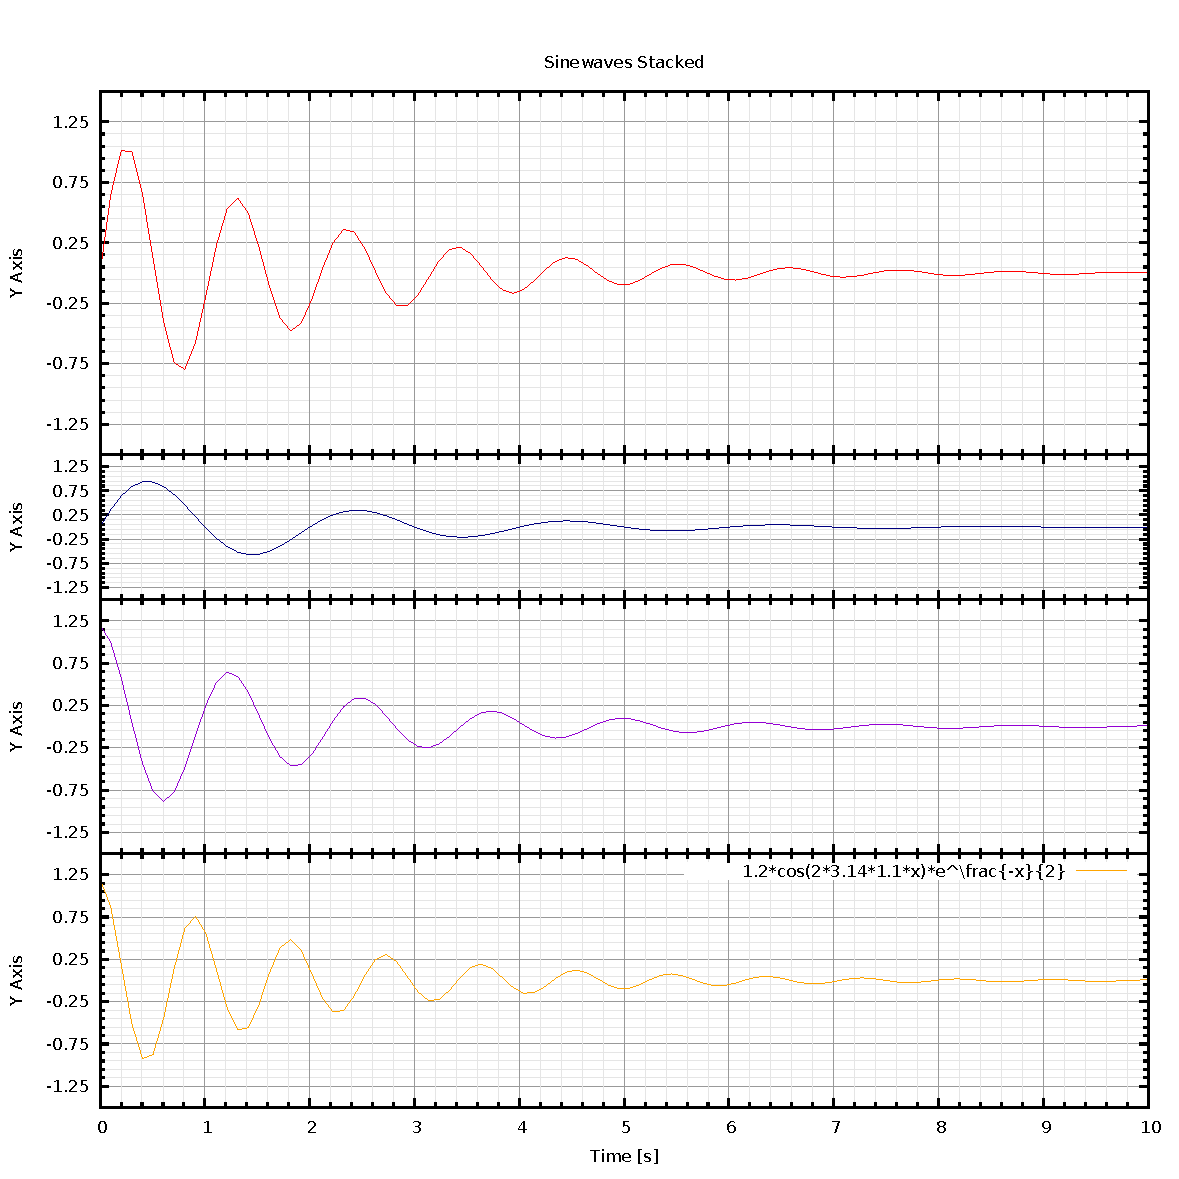
\includegraphics[width=\textwidth]{../Code/MultipleStackedPlots/MultipleStackedPlots.pdf}
\caption{Multiple stacked plots of different sizes.  There is the problem that the y tics don't make it to the top; see \autoref{sec:MultipleSizedPlots} for a working example.}
\end{figure}
\lstinputlisting{../Code/MultipleStackedPlots/MultipleStackedPlots.plt}

\section{Multiple Sized Plot On One Page, Mini Stacked Plots And Correct y Tics} \label{sec:MultipleSizedPlots}
\begin{figure}[!hbtp]
\centering
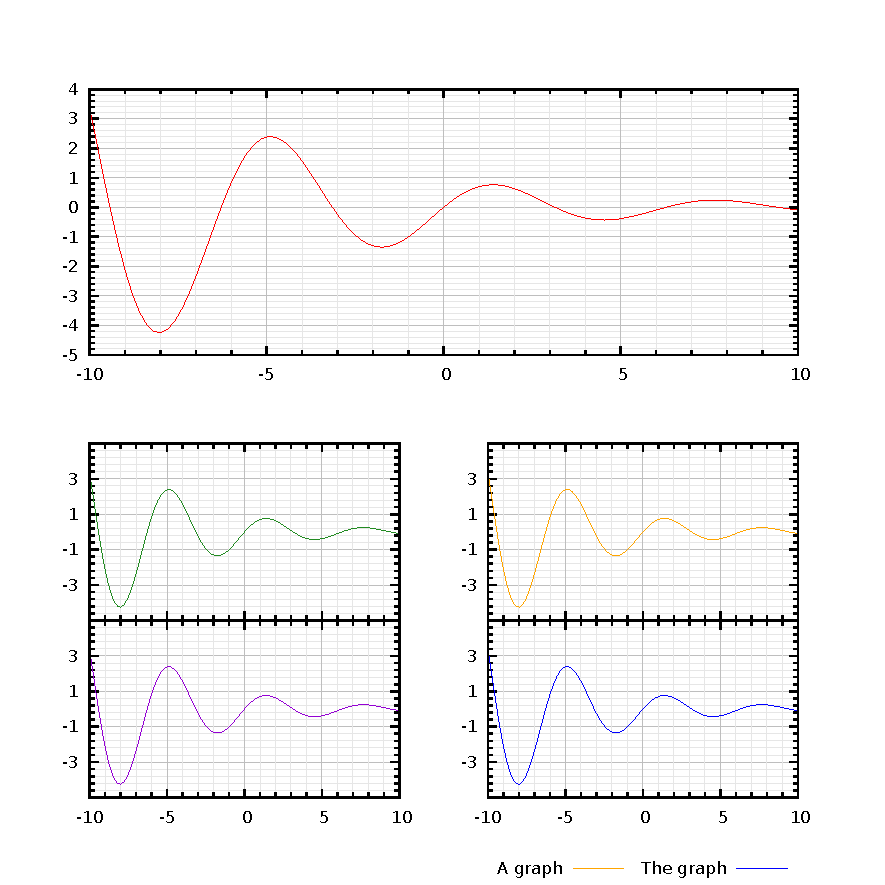
\includegraphics[width=\textwidth]{../Code/MultipleSizedPlots/MultipleSizedPlots.pdf}
\caption{Multiple sized plot on one page, mini stacked plots and correct y tics.  See }
\end{figure}
\lstinputlisting{../Code/MultipleSizedPlots/MultipleSizedPlots.plt}
In order to generate the correct y-tics, the following Ruby script is used.
\lstinputlisting[language=Ruby]{../Code/MultipleSizedPlots/GnuplotMajorMinorTicsLastMajorHidden.rb}

\end{document}
